% !TEX root = ../../thesis.tex


\chapter{Education} % (fold)
\cleanchapterquote{New technologies help students navigate the creative thinking spiral.}{Mitchel Resnick}


\section{introduction} % (fold)
During the last 10 years, the way we learn has deeply changed. Indeed, thanks to the very large democratization of internet, anyone with a connection can access the whole humanity knowledge in just a couple of second. Also a lot of website were made toward this direction. The most famous one is Wikipedia, a community encyclopedia with a non stop growing in quantity and quality. But this internet of knowledge is being also more and more applied to the learning with online free courses such as the Khan Acamedy for primary to high school but also for university we can cite also MIT open course ware (OCW) or open Yale courses.
In france, it is still the begining of this education alternative, a first step was done in the end of October 2013 with the creation of the website France Université Numérique, trying to promote the developement of MOOC teaching in France.

Finally teaching computer science in schools is needed.

\begin{quotation}

    It has become commonplace to refer to young people as “digital natives,” because of their apparent fluency with digital technologies15. And, indeed, many young people are very comfortable sending text messages, playing online games, and browsing the web. But does that really make them fluent with new technologies? Although young people interact with digital media all of the time, few of them can create their own games, animations, or simulations. It’s as if they can “read” but not “write.”

    As we see it, digital fluency requires not just the ability to chat, browse, and interact, but also the ability to design, create, and invent with new media~\cite{resnick2008sowing}.To do that, you need to learn some type of programming. The ability to program offers many important benefits: it greatly expands the range of what you can create (and how you can express yourself) with the computer, while also expanding the range of what you can learn. In particular, programming supports the development of “computational thinking,” helping you learn important problem-solving and design strategies (such as modularization and iterative design) that carry over to non-programming domains18. And since programming involves the creation of external representations of your problem- solving processes, programming provides you with opportunities to reflect on your own thinking – and even to think about thinking itself~\cite{disessa2001changing}

    \signed{Mitchel Resnick and al. Scratch: Programming for Everyone~\cite{resnick2009scratch}}

\end{quotation}


For this purpose robot are a great tools as they permit to see in the real world the meaning of code line. Also the motivation to make something move helps to overcome the annoying code synthax.
We are learning in a meaningful context and its the best way of learning.

In robotic, basic geomtric calculus has sense.

To introduce computer concepts to children, MIT Media Lab developped Scratch~\cite{resnick2009scratch} forked by Berkeley into Snap an extended reimplementation of Scratch wich makes it suitable for a serious introduction to computer science for high school or college students. With its block interface, it allows to code by combining block such as Lego one.


Also, the novel society revolution is in progress around the internet of things. Indeed, the amazing emergence of Fablabs and the developement of low cost open source rapid prototyping tools open the field of personnal fabrication. Soon, as we can share knowledge or information we will be able to share real object. So we can think, it will have a great interaction with MOOC to learn with experimental setup easily reproducible at home or in Fablab.


\section{Education and the Poppy project} % (fold)

The Poppy platform was initially design for research purposes and even more specifically for studying biped locomotion and human-robot interaction. However, right from the beginning, we decided to make it a context of open science to share both our research and a tool for research.

This choice as strongly impacted the way we design our platform. Indeed being simple to use, easy to build and control, modular, 3Dprintable and as plug'n'play as possible lead to the development of tools hardware (Poppy) and software (pypot) which can be also used by non-expert people. Thus the Poppy project ADN is to



The Poppy Project develops an open-source 3D printed humanoid platform based on robust, flexible, easy-to-use and reproduce hardware and software\footnote{Web page: \url{http://www.poppy-project.org}}. In particular, the use of 3D printing and rapid prototyping technologies is a central aspect of this project, and makes it easy and fast not only to reproducible the platform, but also to explore morphological variants. Poppy targets three domains of use: science, education and art.

Poppy was initially designed with a scientific objective. It was designed to be a new experimental platform opening the possibility to systematically study the role of morphology in sensorimotor control, in human-robot interaction and in cognitive development. Indeed, a suitable design of a robot morphology can greatly simplify control problems, increase robustness, and open new modes of interaction with the physical and social world. Thus, being able to study the body as an experimental variable, something which can be systematically changed and experimented, is of paramount importance. Yet, until recently it was complicated because building a robot relied on heavy and costly manufacturing techniques. 3D printing has changed the landscape of what is possible: Poppy Project transposed it to humanoid robotics, and it is now possible to explore new body shapes in just a few days. It enables and simplifies the experimentation, the reproduction and the modification of the morphology in research laboratories. It also allows collaborative working, sharing and replication of the results on these issues between laboratories. The ambition is to become a reference platform for benchmarking and dissemination of scientific results.

Thanks to the fact that it integrates advanced and yet easily accessible techniques in an embodiment that motivates students and the wider public, this platform also meets a growing societal need: education and training in technologies combining computer science, electronics and mechanics, as well as a training tool to the emergent revolutionary 3D printing process. With its openness, its design and its rather low-cost, Poppy provides a unique context for experimentation and learning of these technologies in a Do-It-Yourself (DIY) approach. Several experiences with Poppy in secondary, high schools, science museums and Fablabs in France and abroad are already underway and will be discussed in the incoming sections.

Finally, the possibility to easily modify both the hardware and the software also makes Poppy a useful tool for artistic projects working with interactive computerized installations.


Les choix de conceptions que nous avons fait ont entrainé un side effect. En effet, le choix de faire un robot simple, reproductible, plug'n'play, avec une librairie simple et le tout open source ouvre le champ des possibles dans l'éducation.

We are motivated by showing a honest representation of the robotic state of the art and we are convinced that we could still interest people just by leading them to the process of creativity and pionner exploration.

By doing they will see the emergence of complex scientific challenge and so can make them to question themself on how theyr work. Robot are kind of mirror and a way for our brain to understand how itself work on an experimental setup.

% section education_and_the_poppy_project (end)

%context

En effet, avec un robot modulaire et open source comme Poppy il est possible d'extraire des points d'interets, de l'étudier, de le modifier et de le tester. Evidemment, la forme humanoide de Poppy rend le projet ambitieux et excitant pour des étudiants.


%Needs
In 20 years, internet changed the way we learn. The educationnal system certainly needs to change at some point.

In a world where we can access the whole humanity savoir in seconds right from our smartphone, the need of education for children ...

Also as we saw in the chapter ref, now the way we produce thing is also changing and it is just a matter of time (certainly short), before students will be also able to access rapid prototyping tools at their home.

During our meetings with some educationnal team, it appeared what they were more and more going from lectures to
group projects.

% Tasks

The Poppy platform seems well suited to this new kind of education. Indeed, it is fully open source so teacher can explain in detail how it is done, then it is easy to hack it for specific project because the software is programming in python, the hardware is 3D printable and the sensors can be easily plugged on the arduino board.

% Objects
In another context, a project between scientific mediation and education was organised has an hackathon in the paris science museum, univers science.

Before the end of this thesis, we get the chance to set up an experiment in a highschool with about 40 students and 3 teachers.



Beyond scientific events such as the Universcience Hackathon, we think the use of open source 3D printed robot such as Poppy can take be an important part for long term educationnal project in university.

Indeed, Poppy is a modular platform, quite easy to use and the open source release allows a deep understanding of state of art technologies. Since october 2013 we have been contacted by several university, engineering school and even high school.


\subsection{Scientific hackathon} % (fold)

On march 22th \& 23th 2014, UniverSciences\footnote{Paris museum of sciences and technologies} organized a hackathon for the general public around the assembly of a Poppy robot (see \figurename~\ref{fig:poppy_universience}). It involved 15 robotic enthusiasts, from children to adults. Participants were dispatched around several workshops during the two days. While a group was dedicated to the actual assembly of the different Poppy parts, others were exploring how to program the robot with the Python software or working on designing and 3D printing hardware improvements.  Aside the workshops around Poppy, several presentations and conferences about robotics were set-up. In this context, participants are not only spectators of a scientific mediation act but also actors.

\begin{figure}[]
\centering
    \subfloat[][Constat]{\includegraphics[height=5cm]{hackathon_intro.jpg}}
    \hfil
    \subfloat[][Conception]{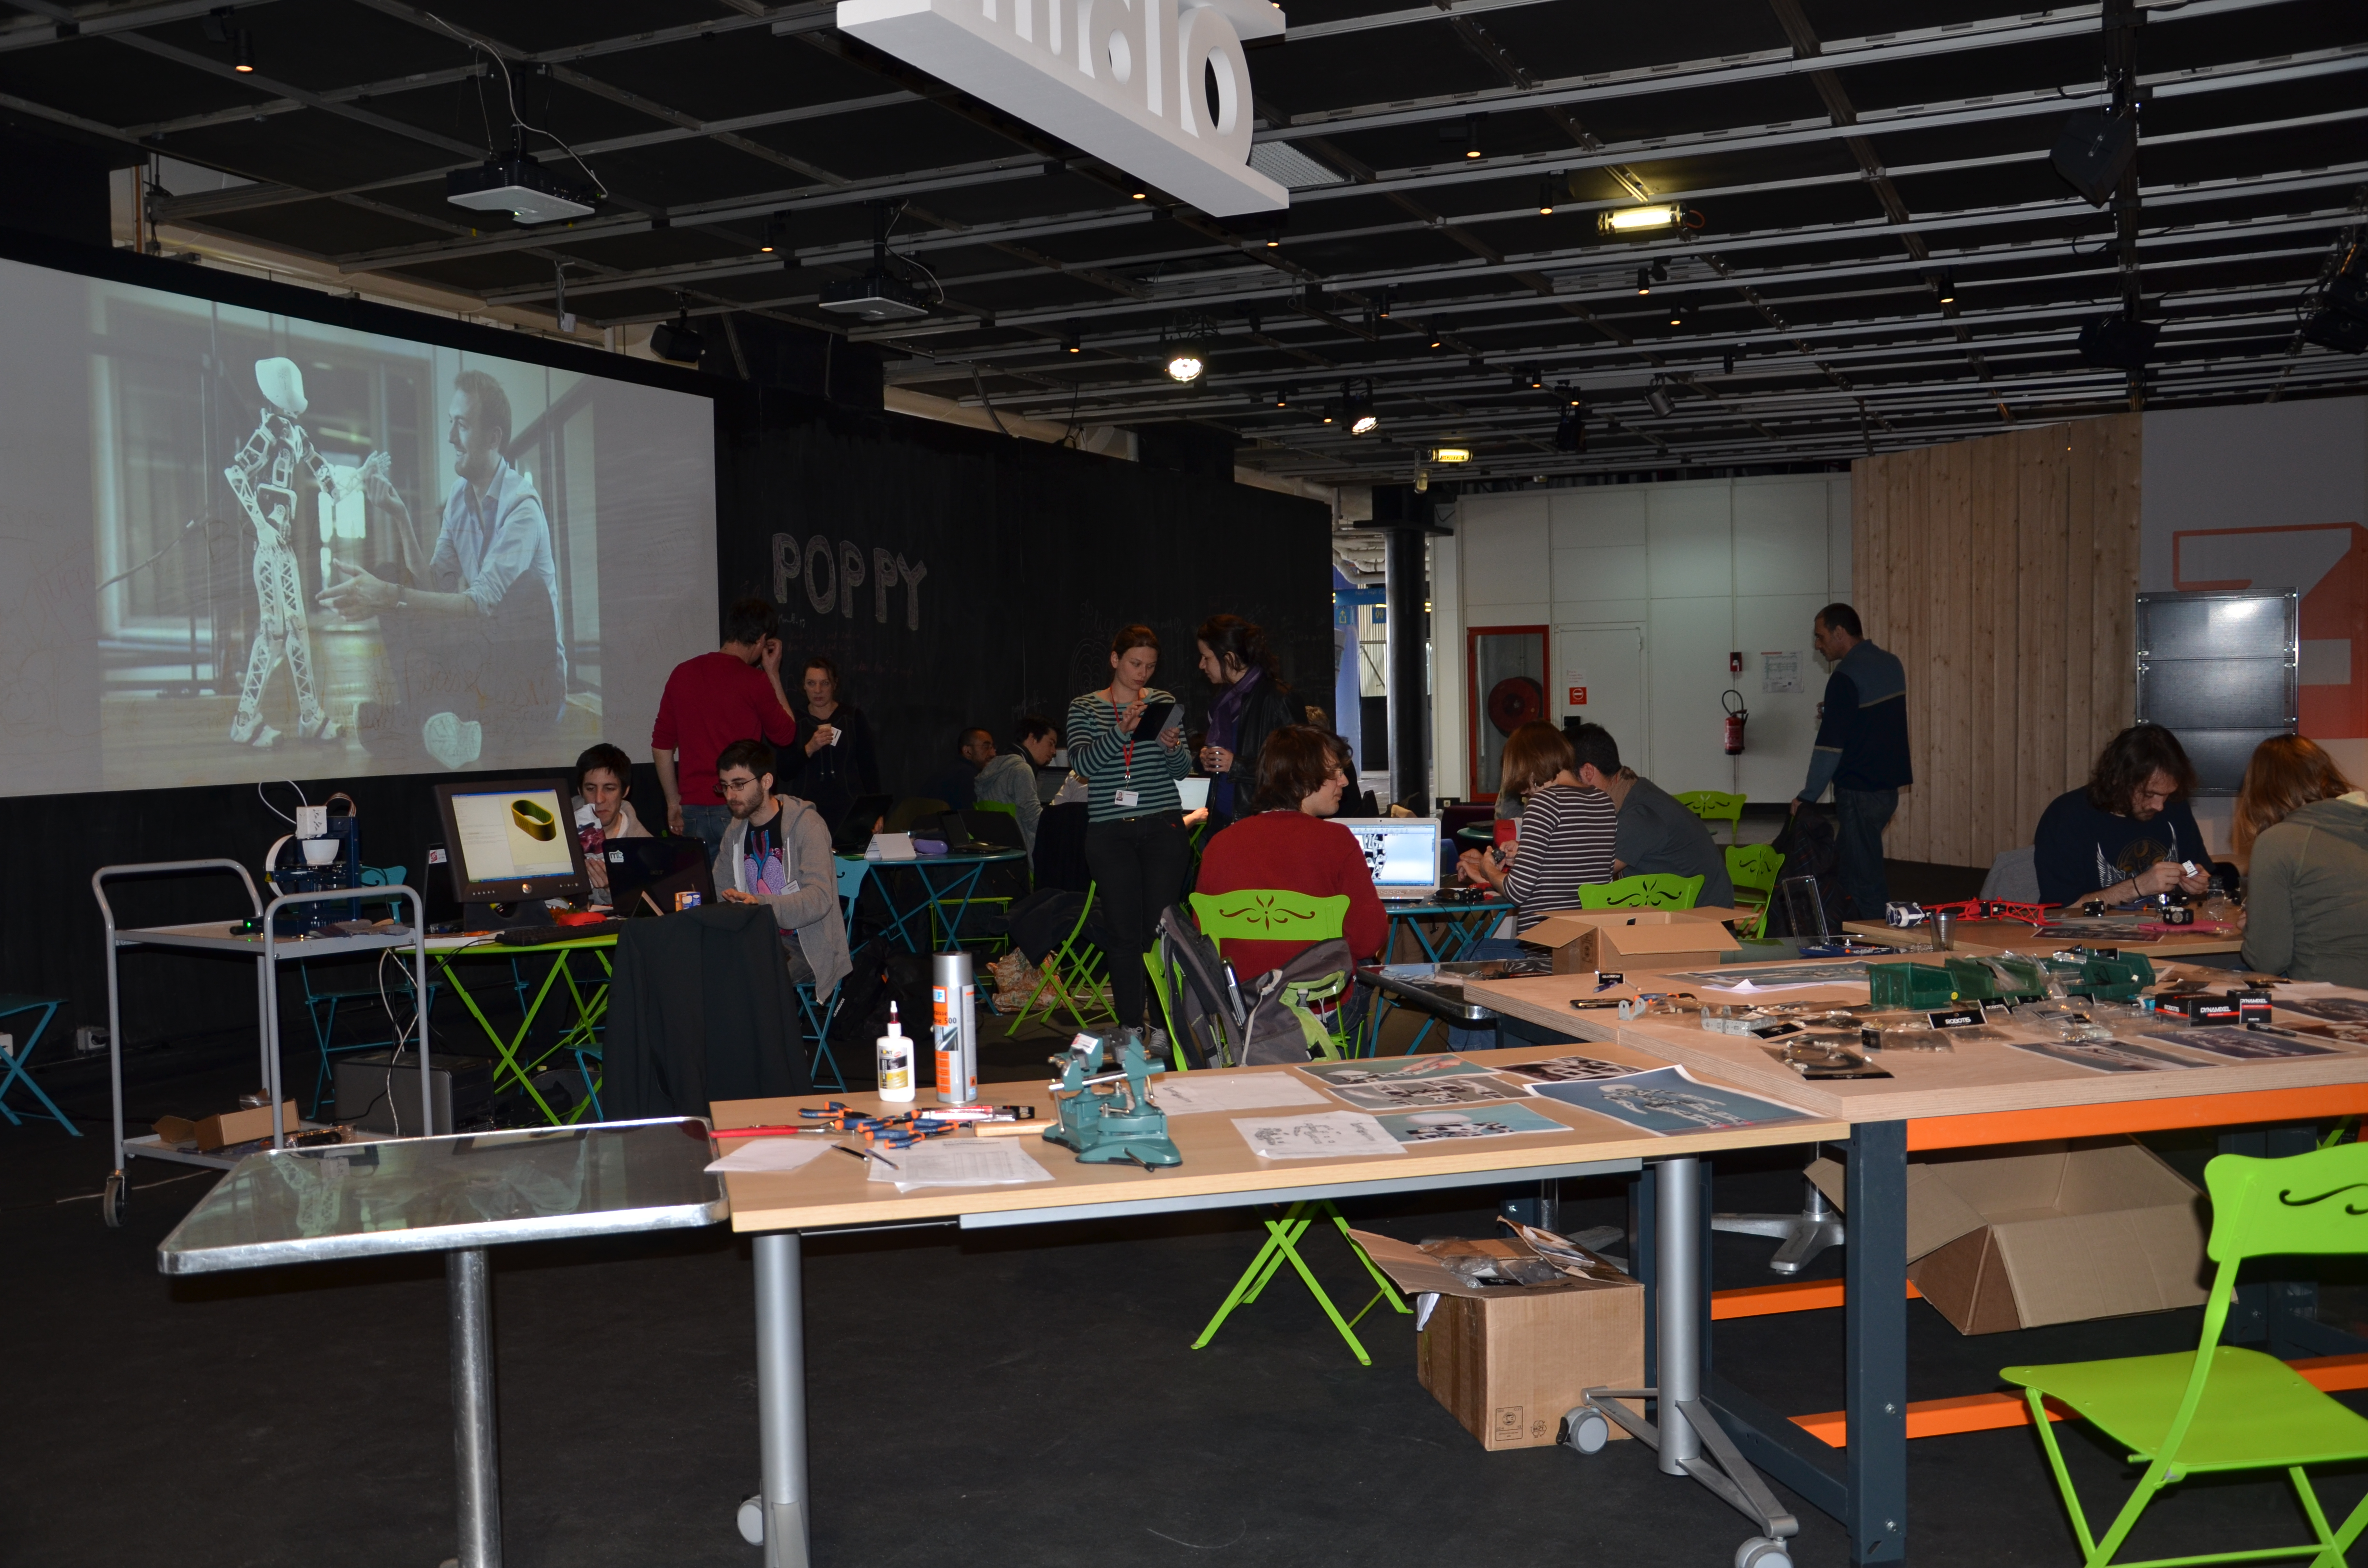
\includegraphics[height=5cm]{hackathon_setup.jpg}}
    \caption{}
    \label{fig:universience_hackathon_orga}
\end{figure}

In two days, this group of new users, self-trained using online documentation have been able to build from scratch the whole robot and make it move using the Pypot library. They even designed a new original semi-passive solution for the ankle joint, as well as a robot helmet which was 3D printed and assembled within the time of the workshop. This experiment did not only show that the platform was easily usable in an educational context with users of all ages, and was rebuildable in two days by a little group, but it also showed high educational value as testified by users and educators (see \url{https://forum.poppy-project.org/t/poppy-project-at-la-cite-des-sciences-et-de-lindustrie/}).

\begin{figure}[]
\centering
    \subfloat[][Constat]{\includegraphics[height=5cm]{hackathon_conception1.jpg}}
    \hfil
    \subfloat[][Conception]{\includegraphics[height=5cm]{hackathon_conception2.jpg}}
    \hfil
    \subfloat[][Production]{\includegraphics[height=5cm]{hackathon_conception3.jpg}}
    \caption{}
    \label{fig:universience_conception}
\end{figure}


\begin{figure}[]
\centering
    \subfloat[][Constat]{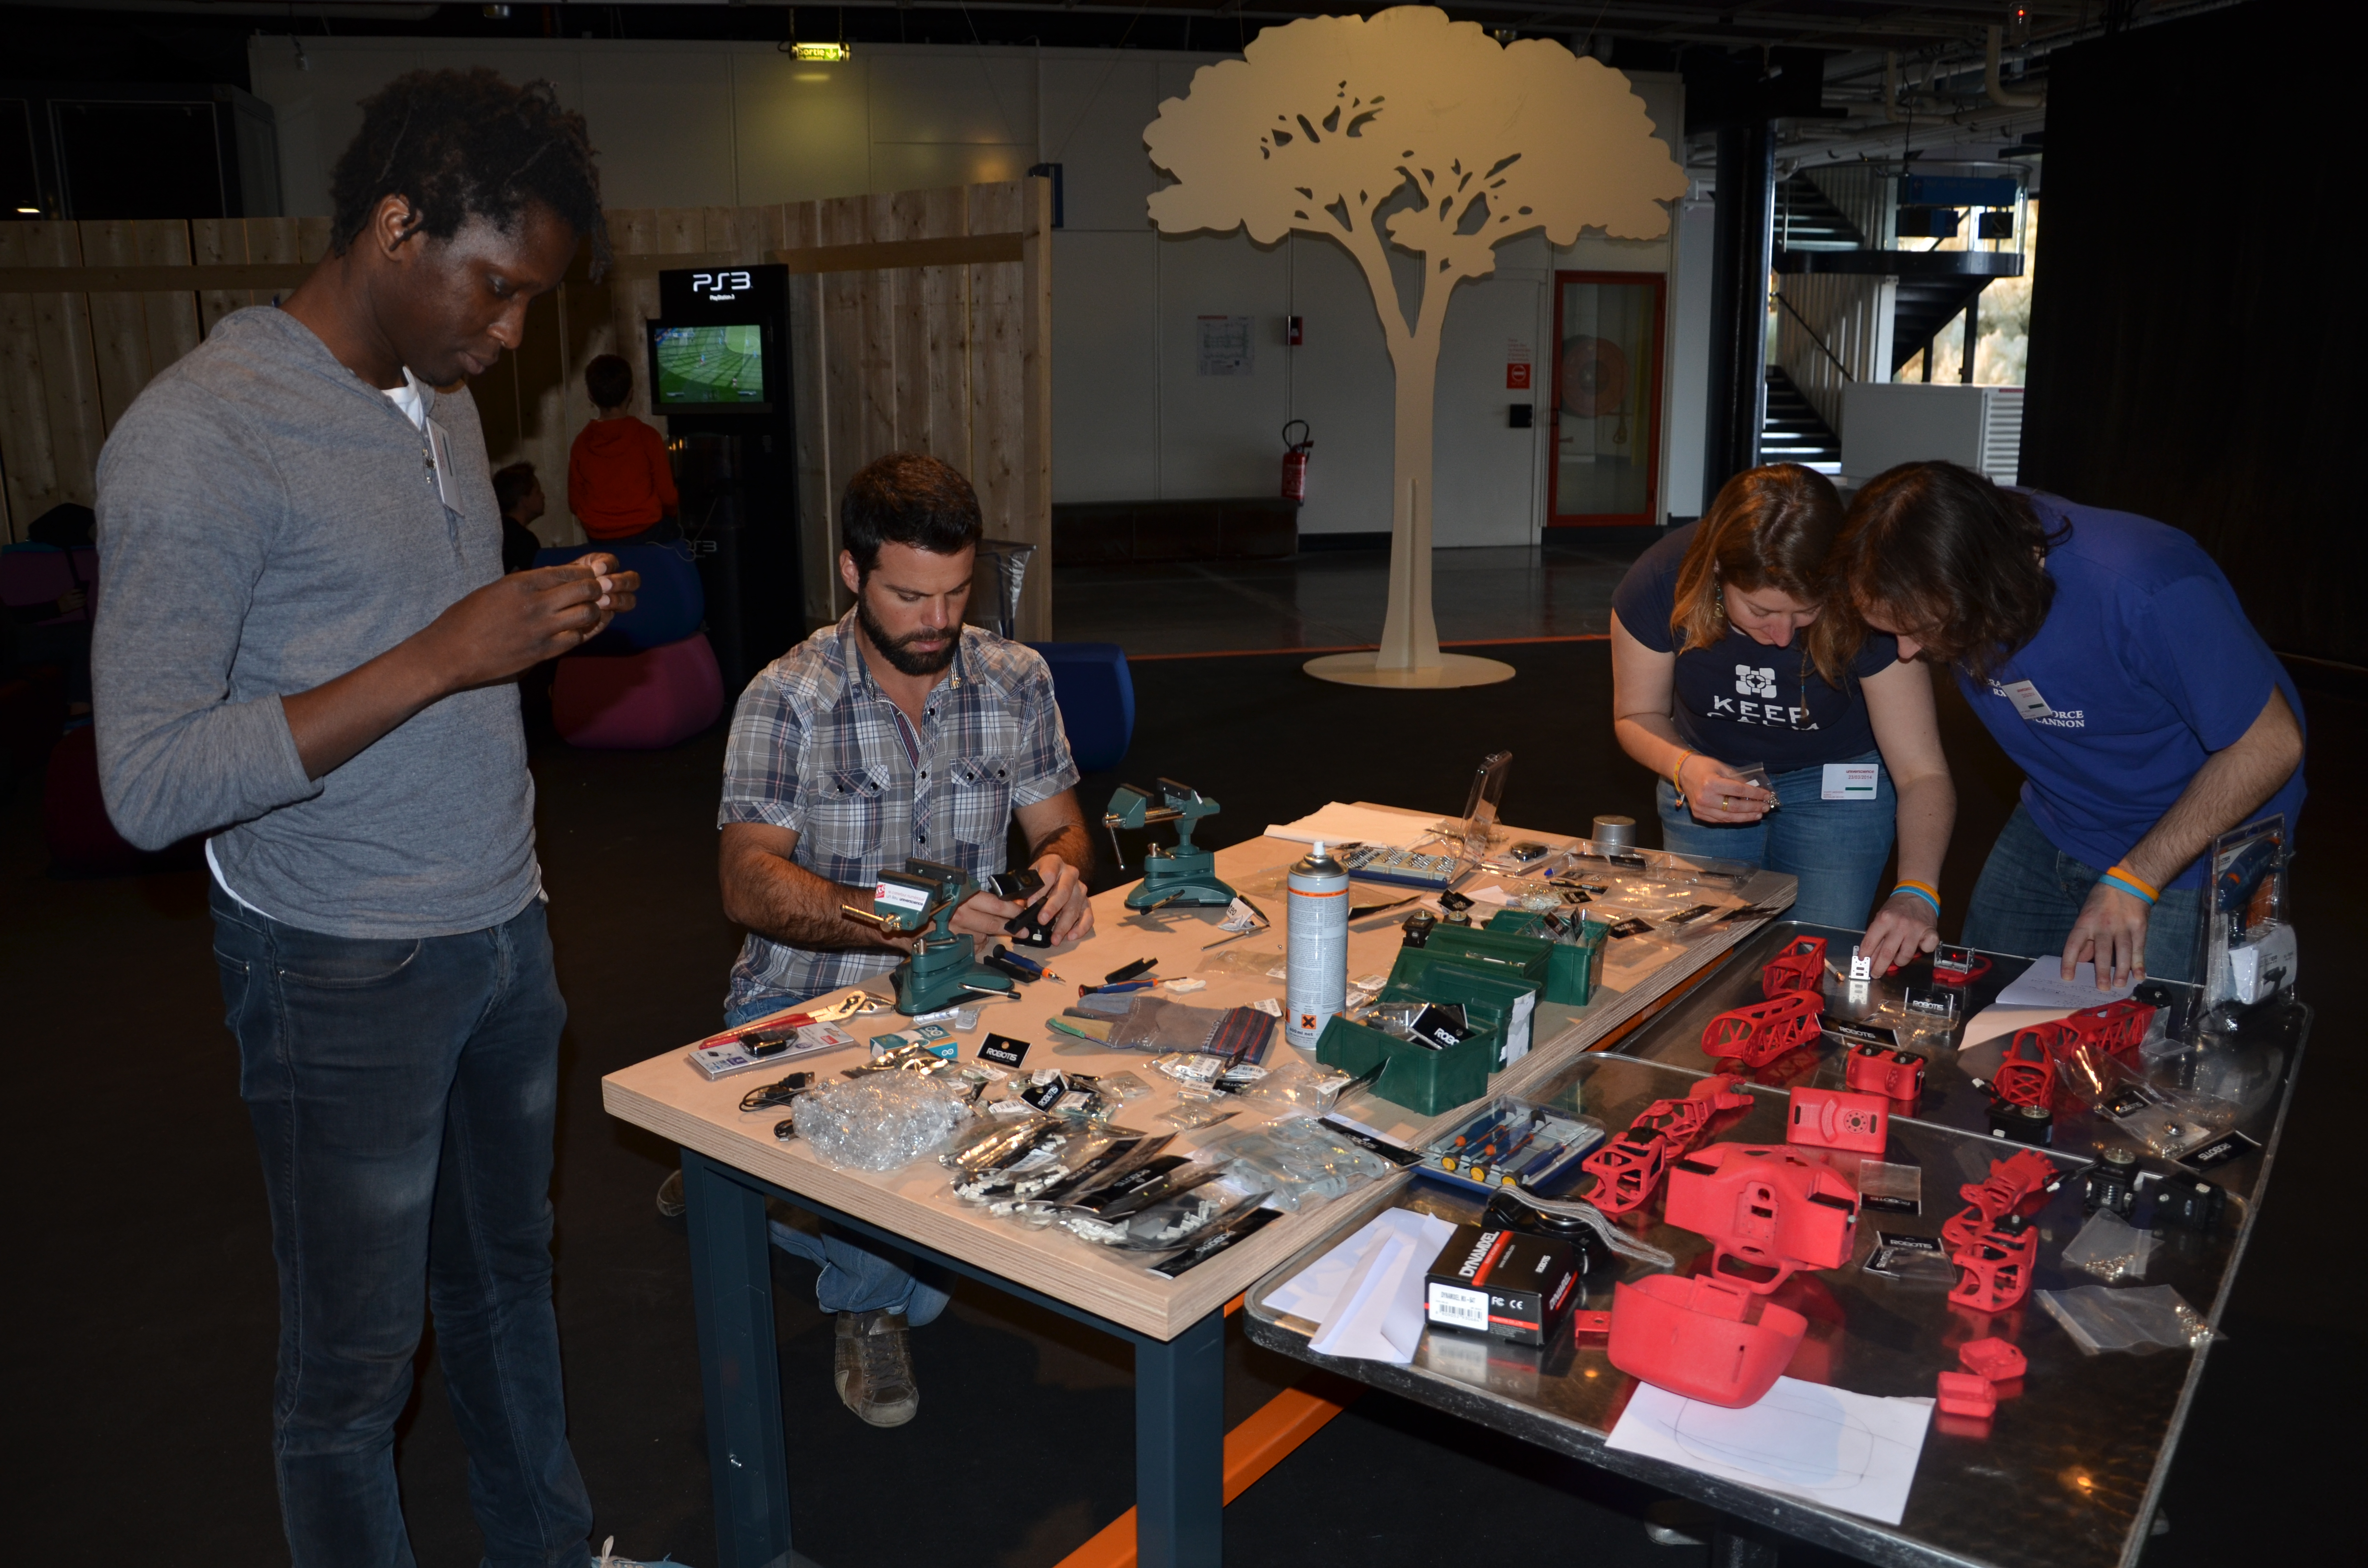
\includegraphics[height=4.5cm]{hackathon_assembly1.jpg}}
    \hfil
    \subfloat[][assembly]{\includegraphics[height=4.5cm]{hackathon_assembly2.jpg}}\newline
    \subfloat[][Production]{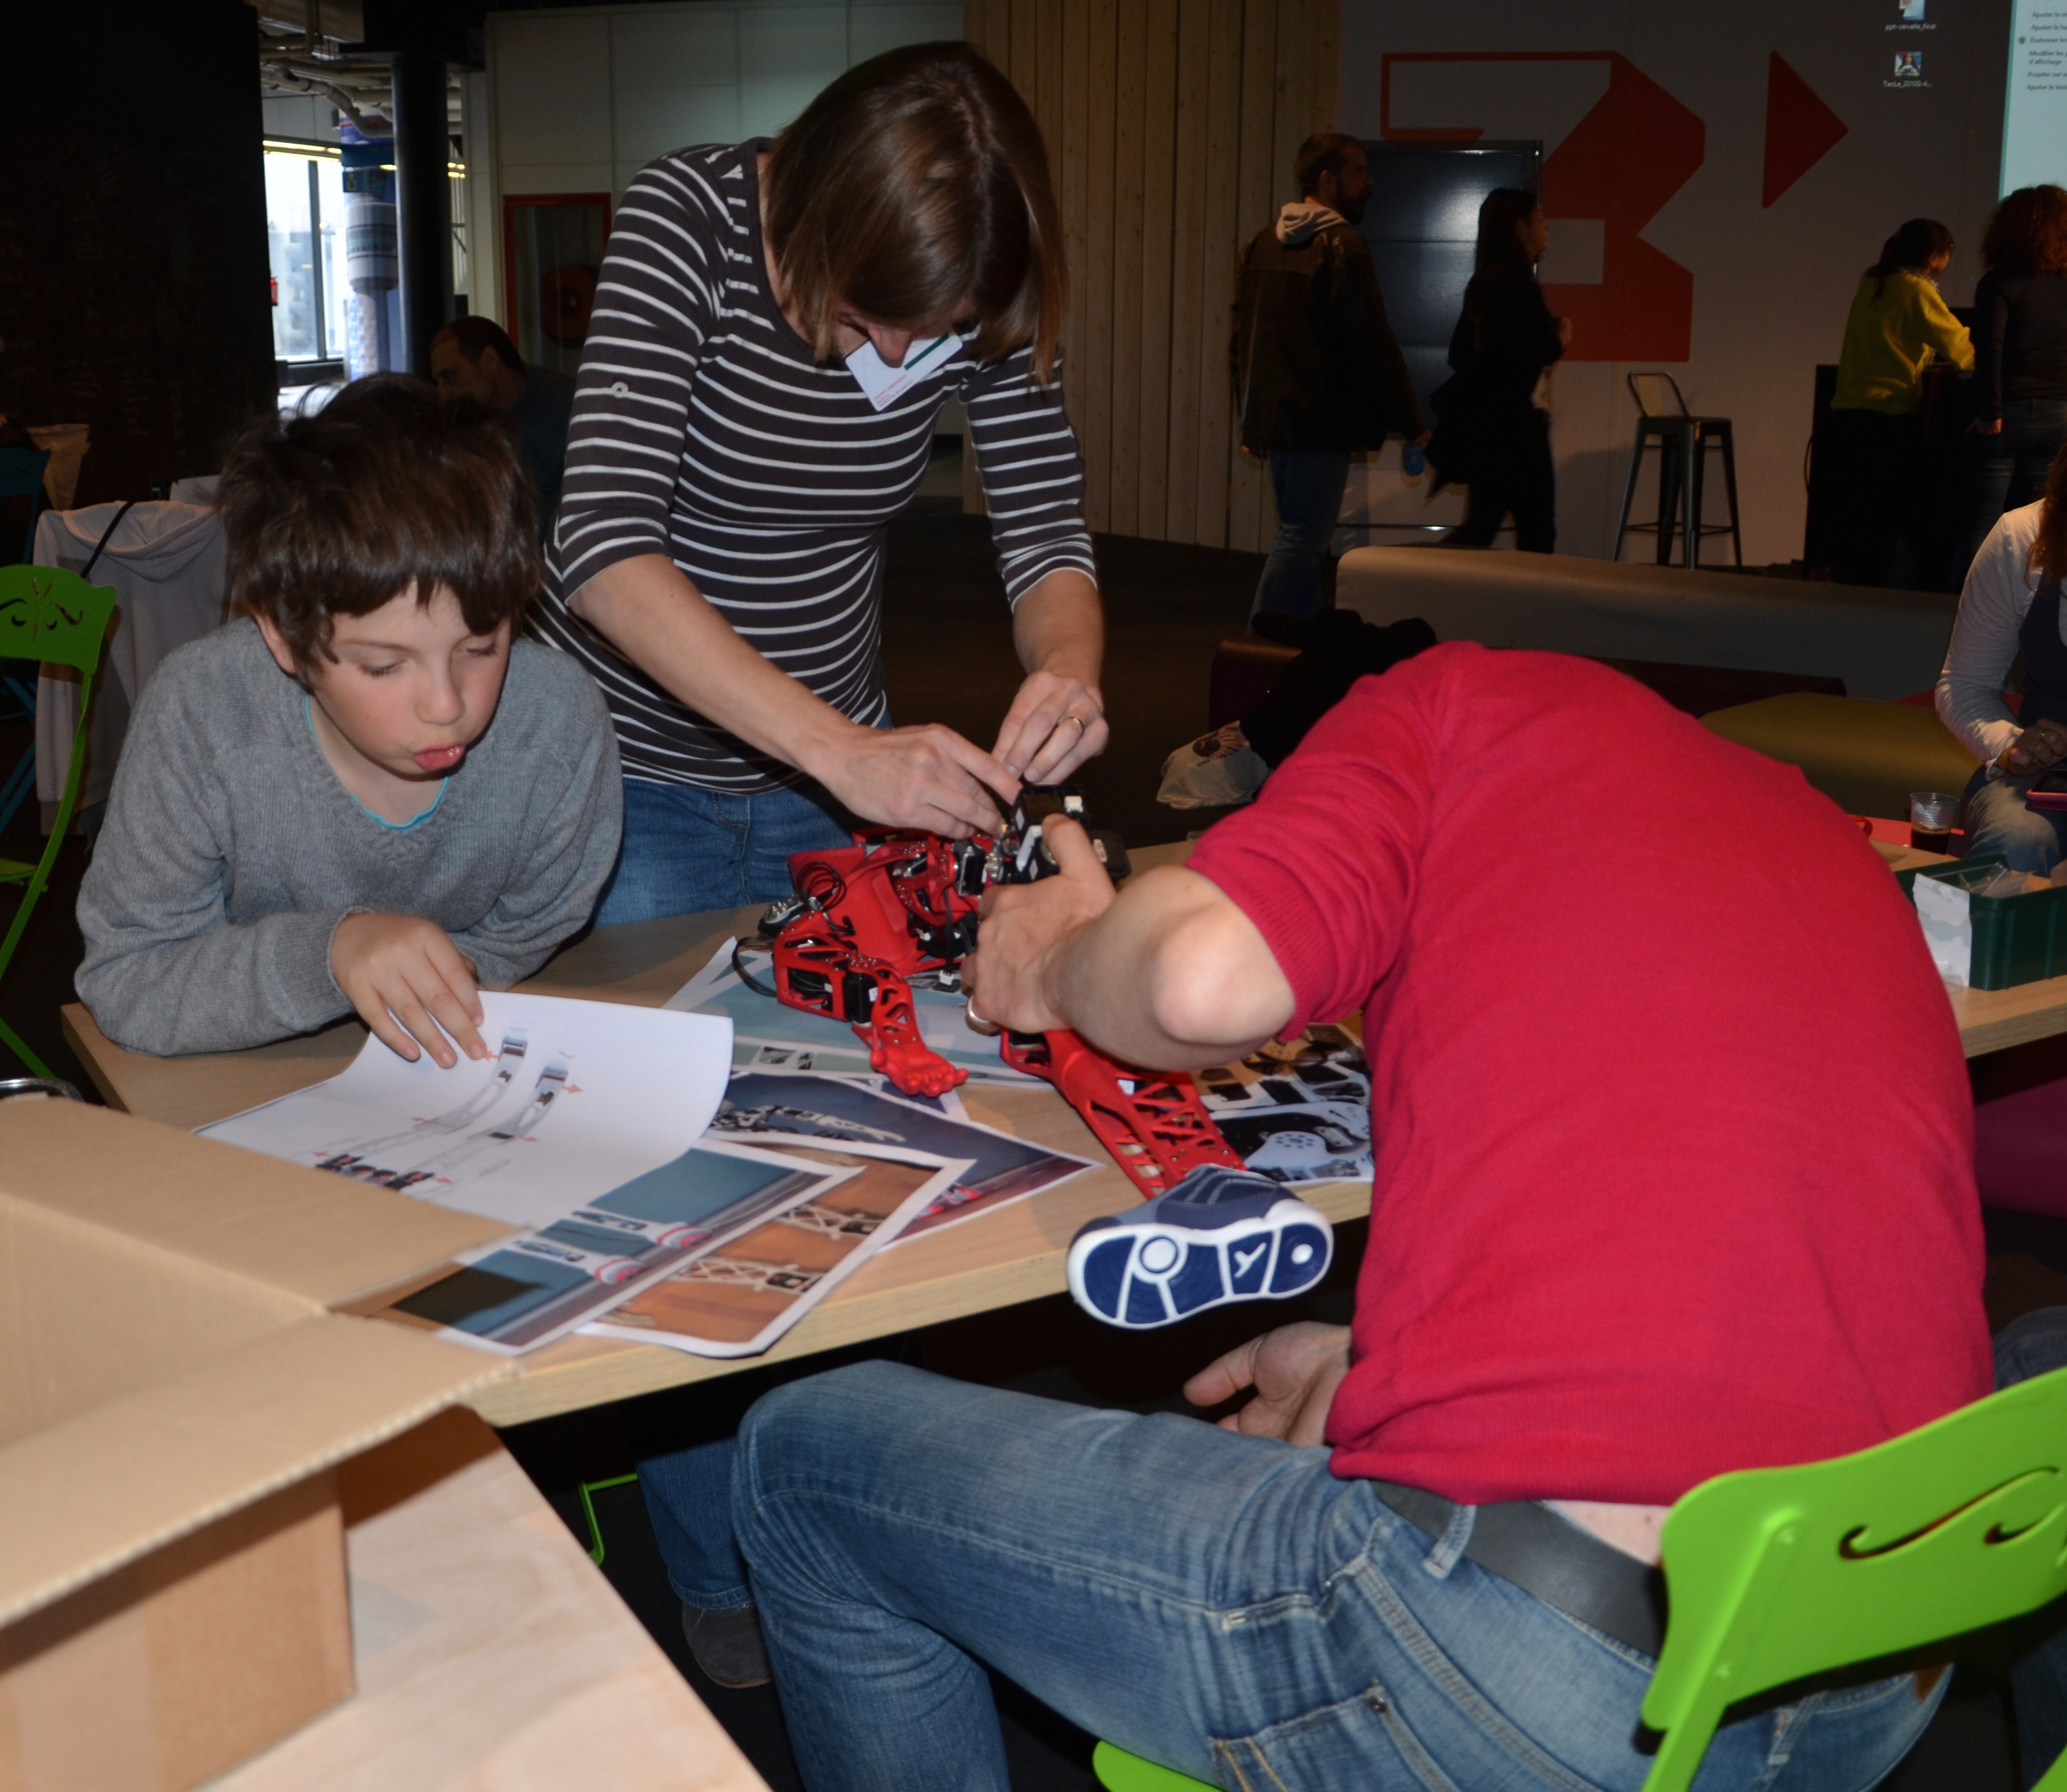
\includegraphics[height=4.8cm]{hackathon_assembly3.jpg}}
    \hfil
    \subfloat[][Production]{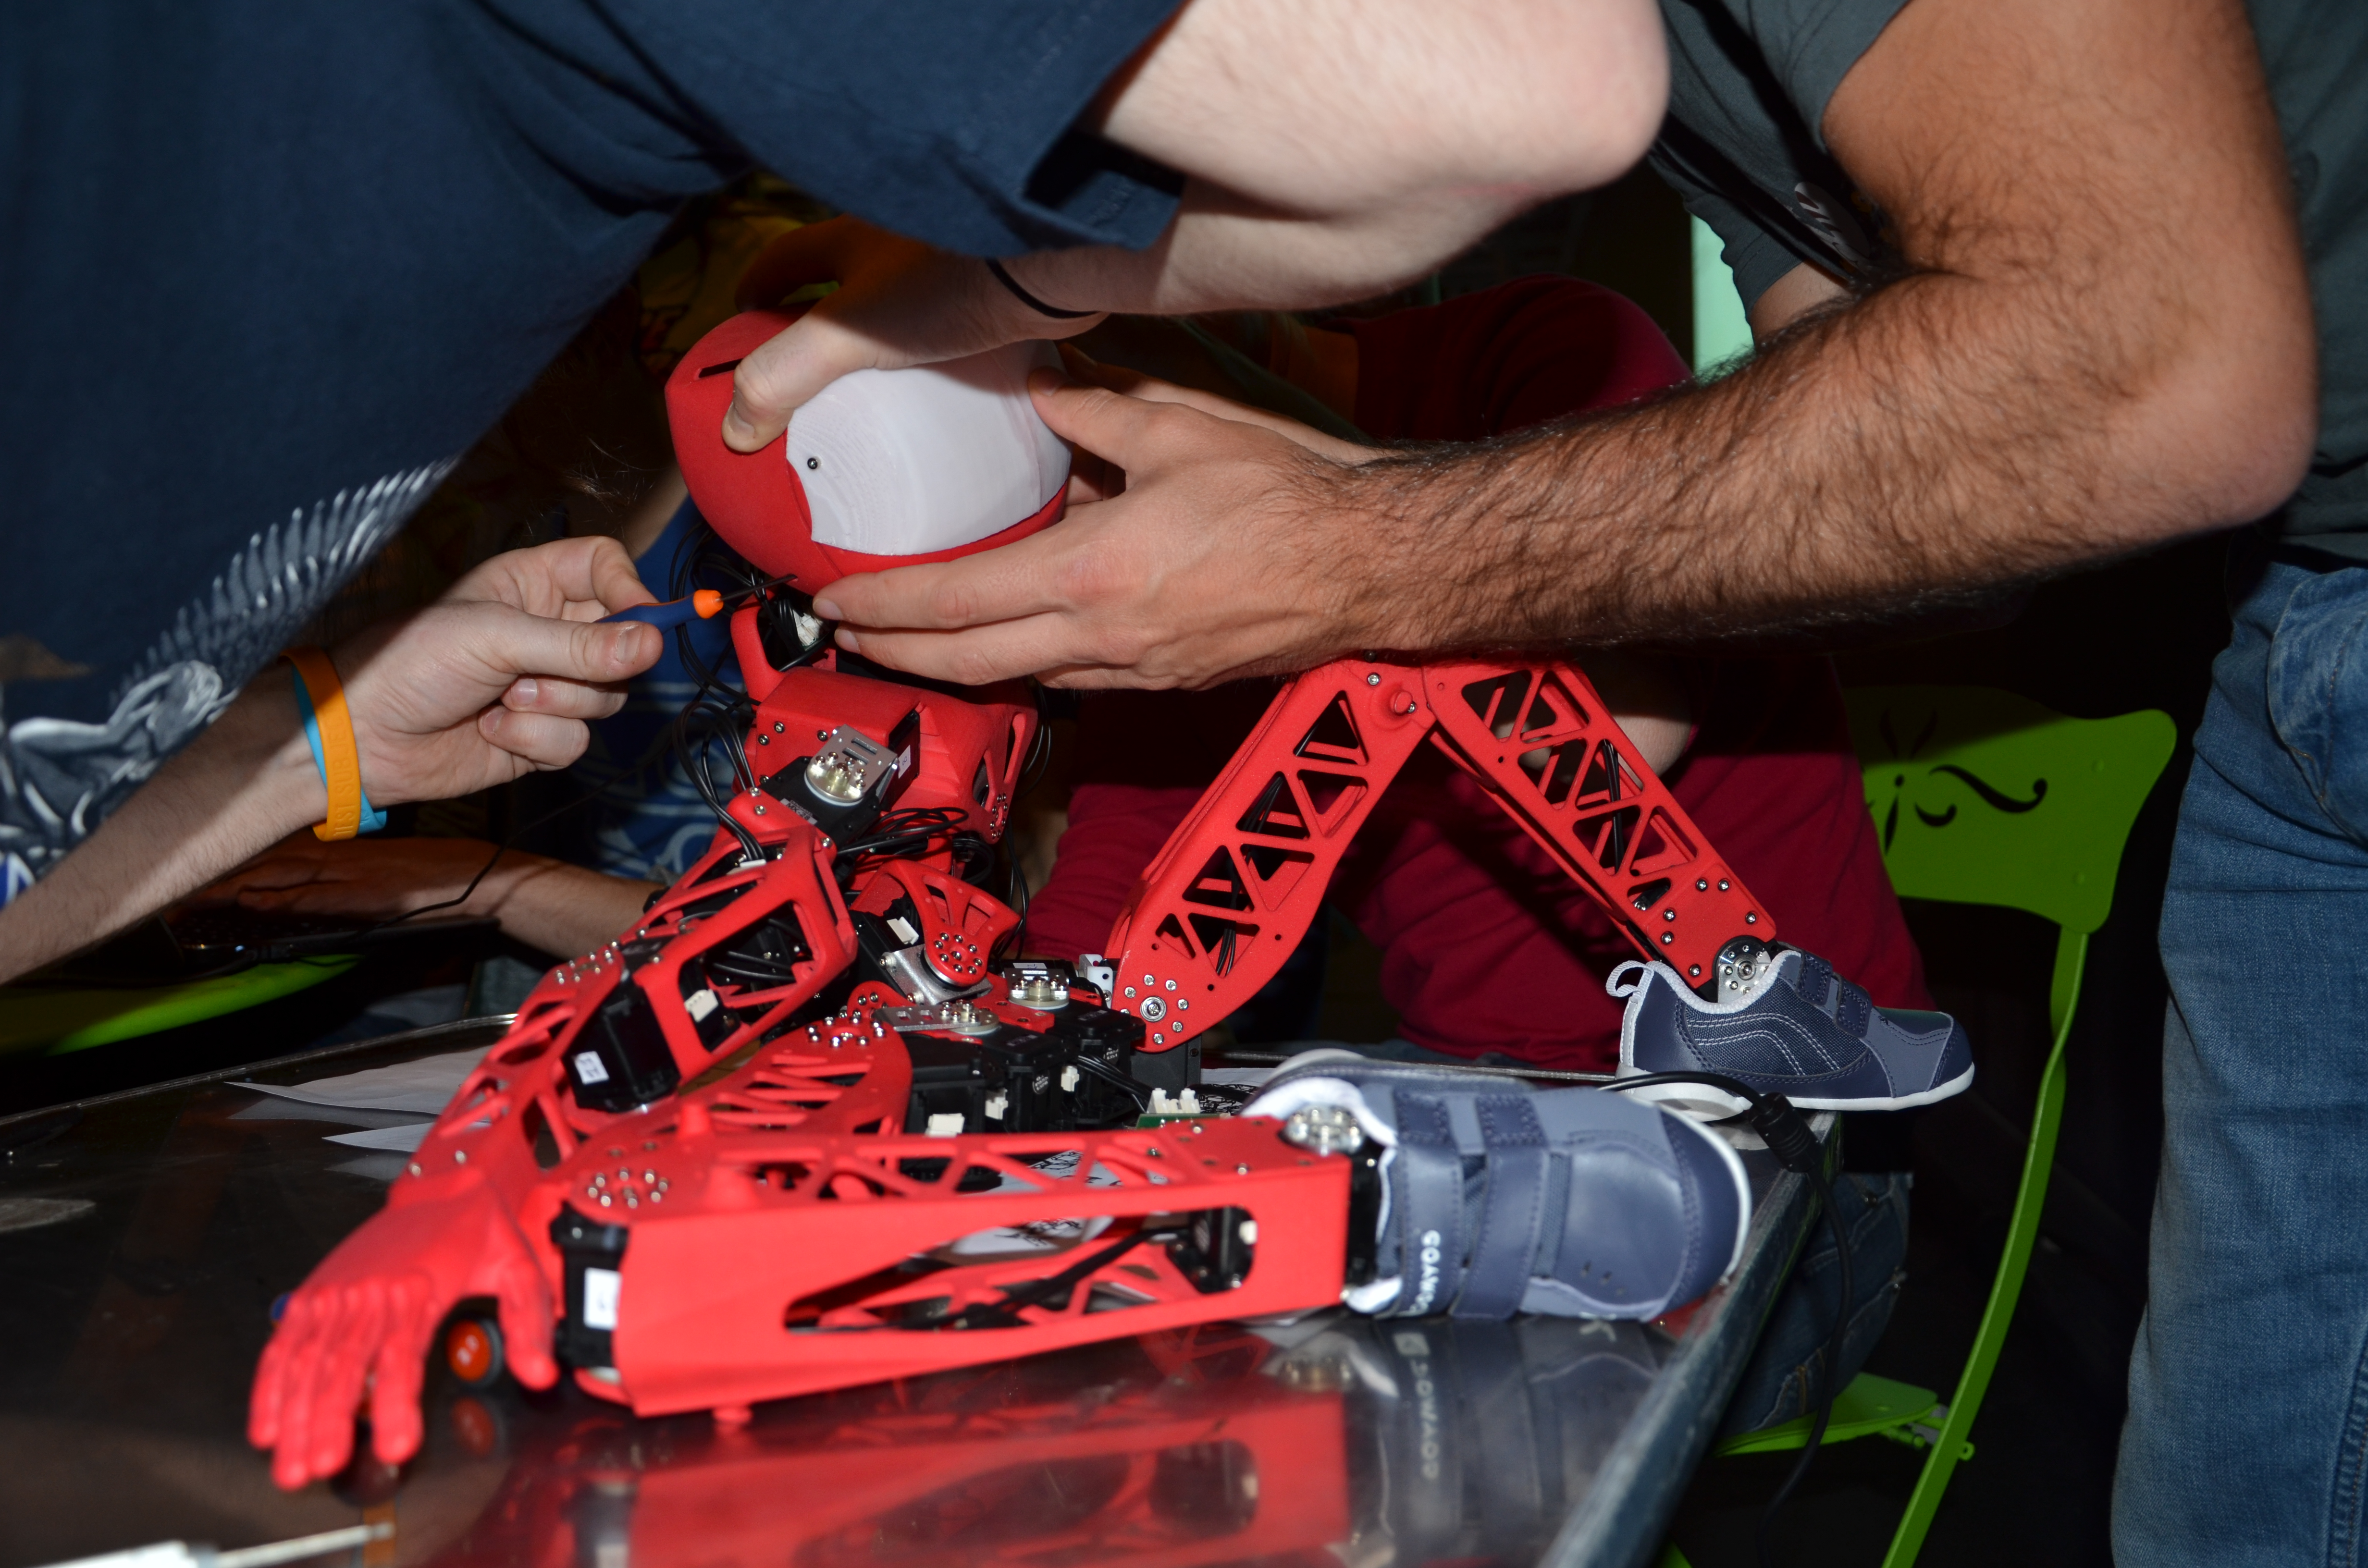
\includegraphics[height=4.8cm]{hackathon_last_screw.jpg}}
    \caption{}
    \label{fig:universience_assembly}
\end{figure}

\begin{figure}[]
\centering
    \subfloat[][Production]{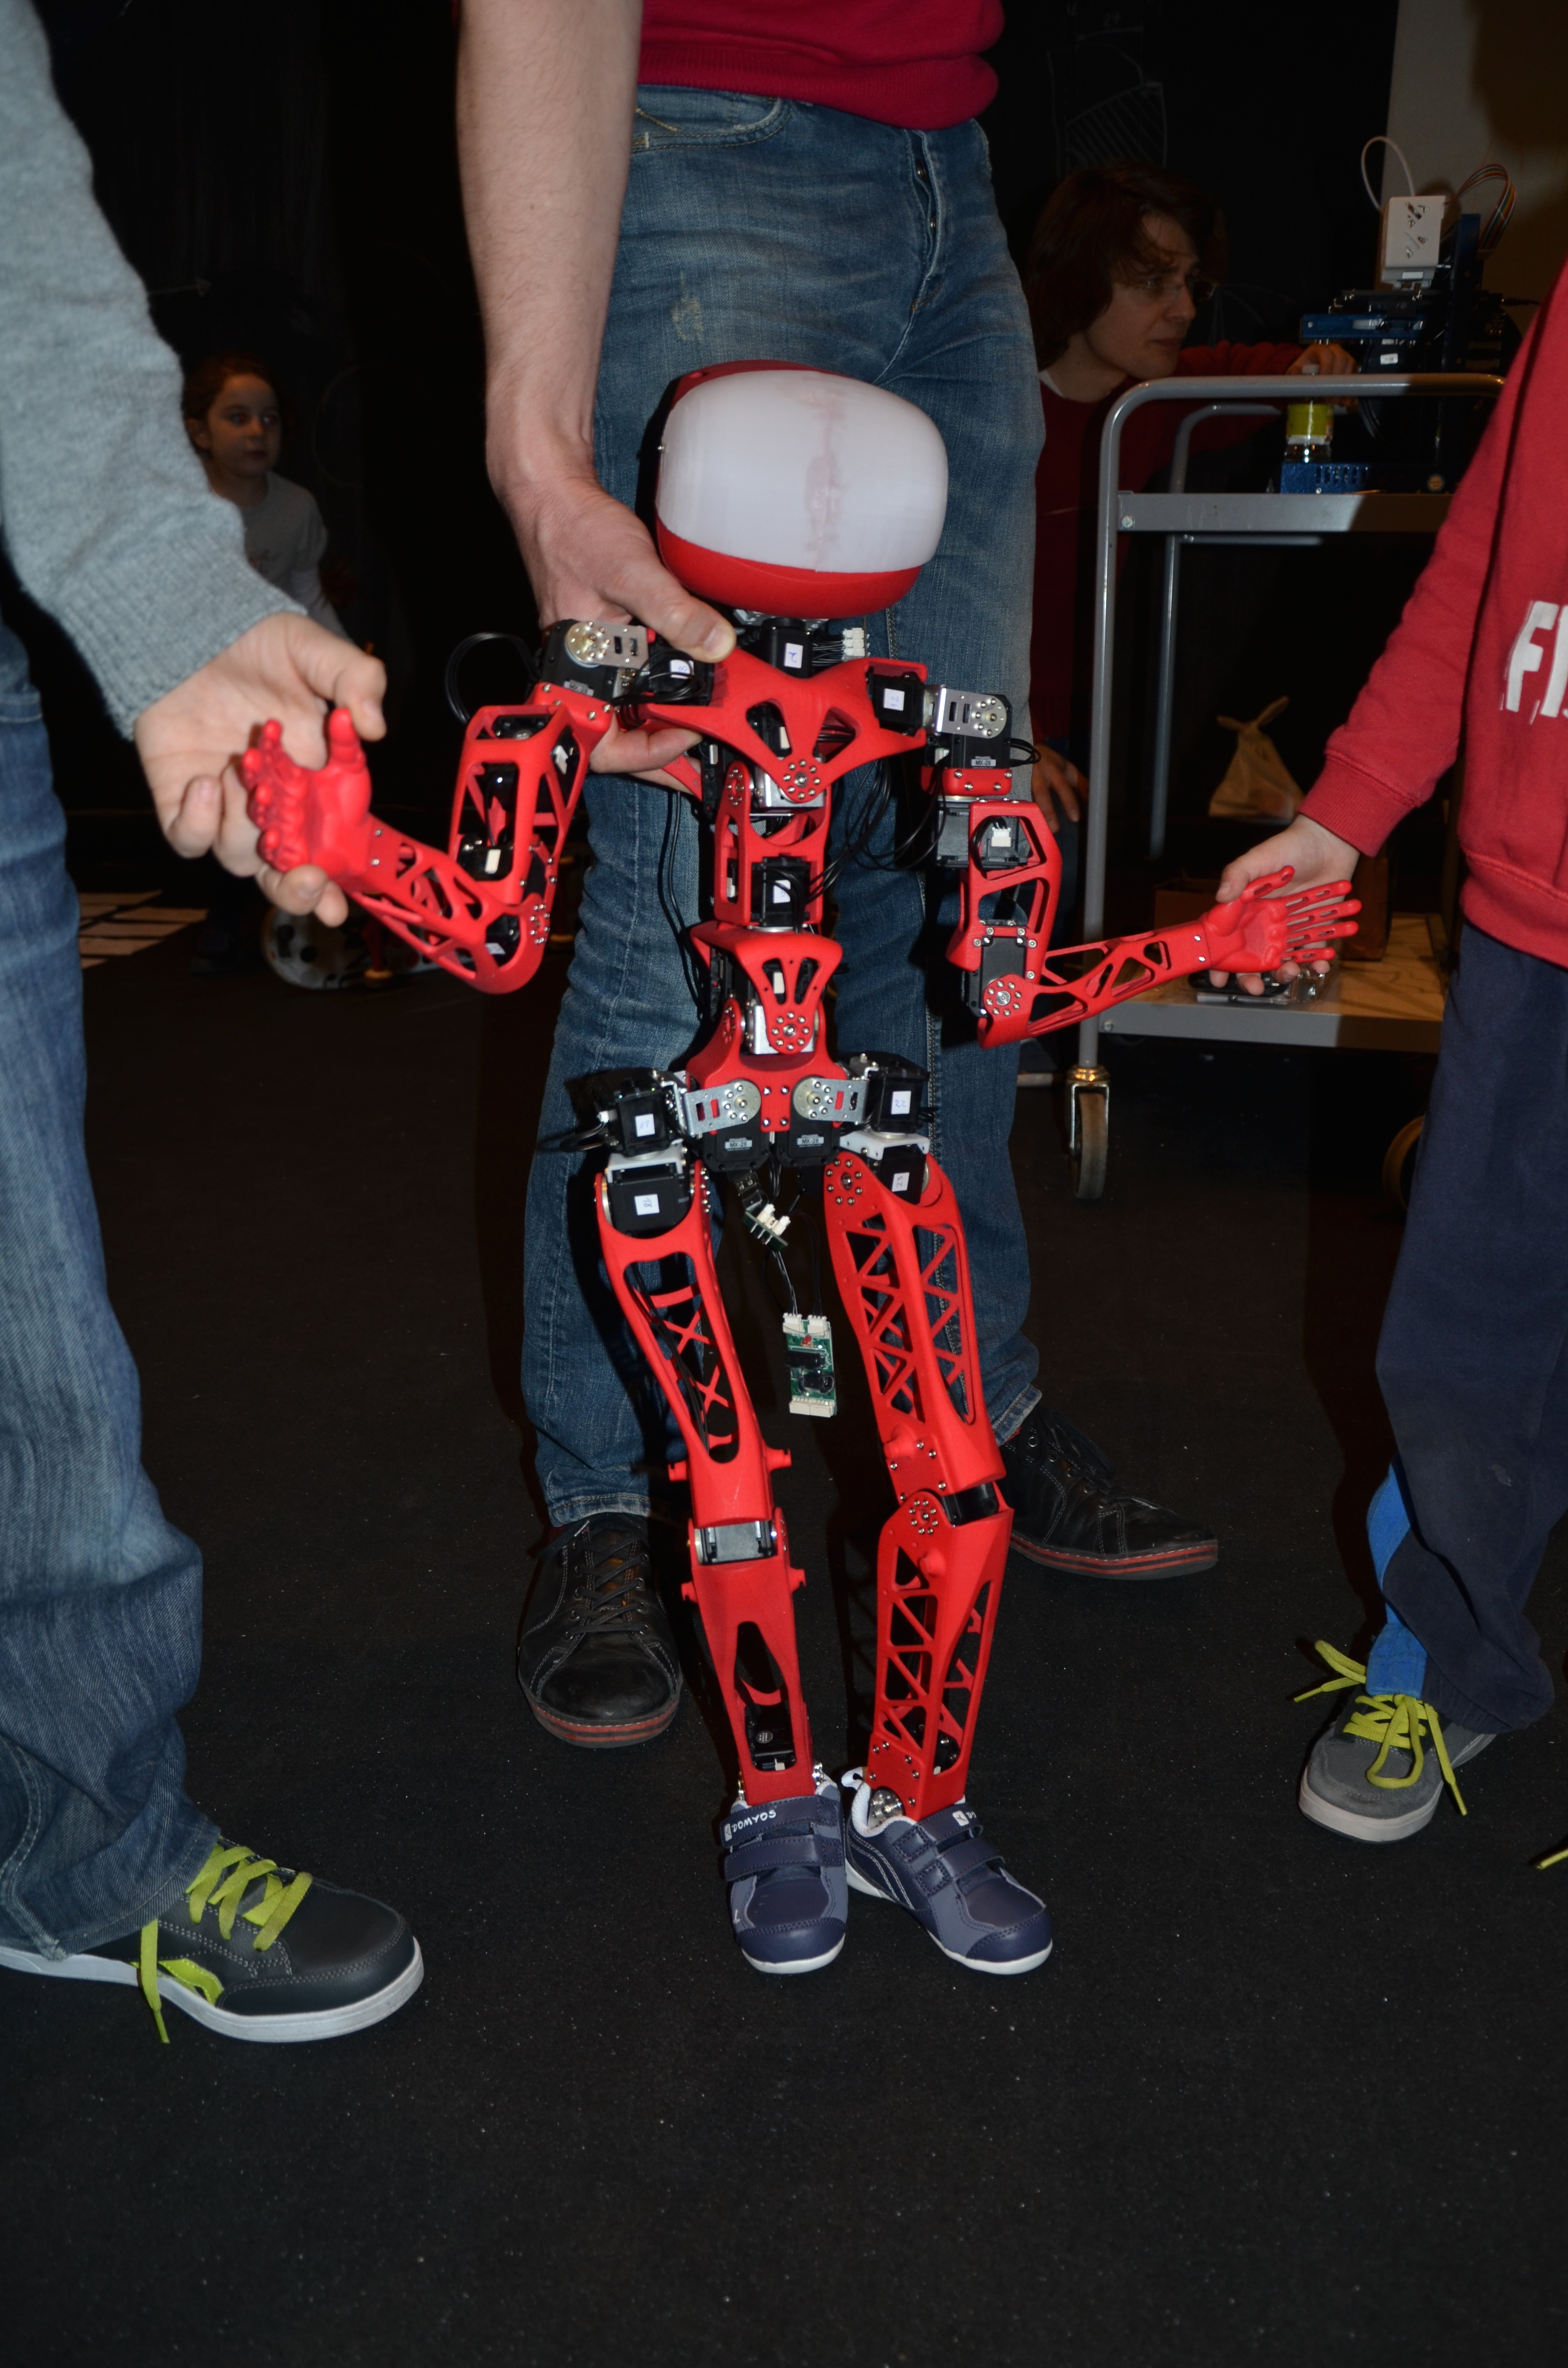
\includegraphics[height=5cm]{hackathon_poppy_assembled.jpg}}
    \hfil
    \subfloat[][Production]{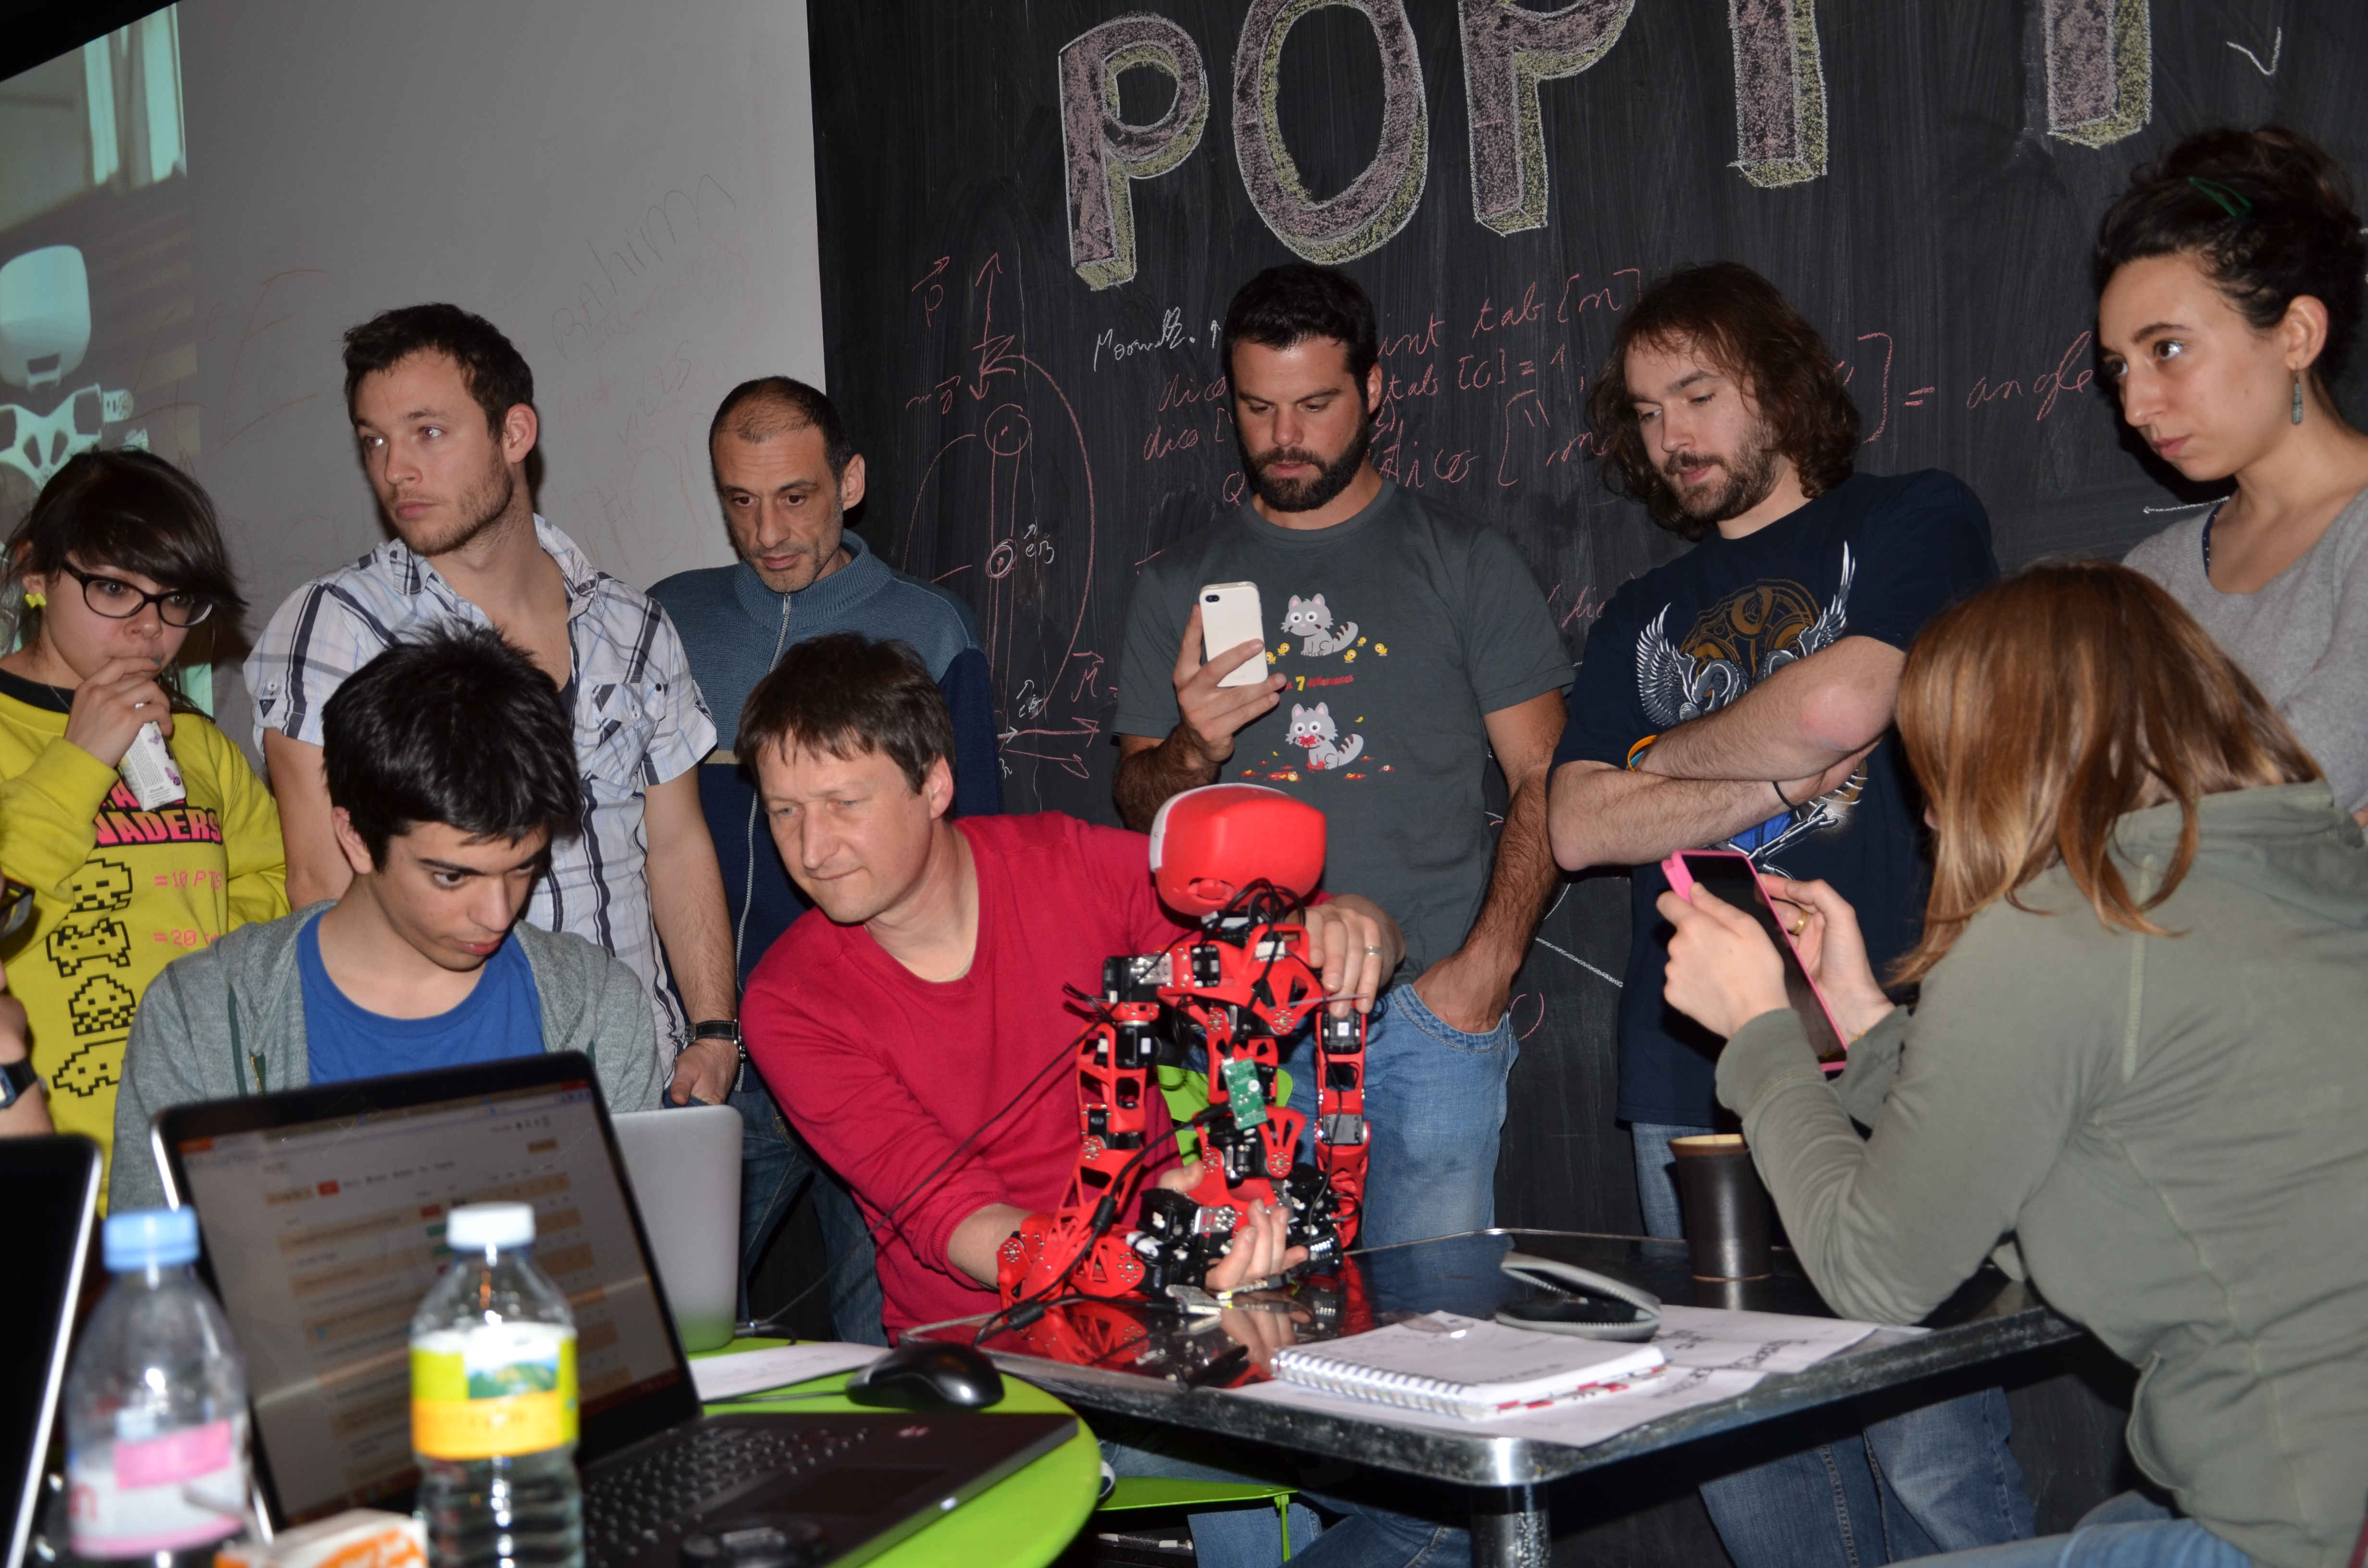
\includegraphics[height=5cm]{hackathon_first_trial.jpg}}
    \caption{}
    \label{fig:universience_conception}
\end{figure}




\section{High school project} % (fold)

After the artistic residency which happened in the Saintonge Sainte Famille high school's chapel (see chapter REF). Some teachers have been interested by the educationnal potential of the Poppy project and wanted to integrate it as a common thread along the school year.

Poppy has been first thought for research purposes and seems to be well-adapted for higher education training. Yet using Poppy in the secondary education seems an overkill as it is expensive and the use of high quality servo-actuators is not justified.

However the experience with high-school students is still interesting and we accepted to take the oppotunity to make a beta test experiment.

\subsection{The experiment course} % (fold)

The experiment concerned near 40 \emph{première STI2D} students (UK equivalent to Year 12) preparing a professional baccalaureate and three teachers from TODO, TODO and TODO specialities.

For the teachers, the main goal was to get the experience of using such tool in a project context and evaluate the the promises and limit for their educationnal mission.

For us, we were interested by the reaction of young students to Poppy and get an opinion on the relevance of Poppy for education at this level. Also, it was a real crash test of our conception (hardware and software) in unexperimented hands.


For this first experiment, we decided to reduce the cost by using only a sub-part of the whole Poppy. For me the most relevant part for high-school students was the upper body (thorax, head and the two arms), because it avoids to work on complex sensori-motor behavior such as balancing and walking while keeping the expressivity of Poppy with the thorax, the head and the two arms. The total cost to get Robotis Dynamixel motors, electronics and 3D prining service was 2500\texteuro (20 \% tax included).

\textbf{TODO: Figure with the upper body of Poppy and the BOM list}


The experiment took place in the Saintonge Sainte Famille high-school on May the 26th \& 27th. The organisation was made around several working groups during three half-days. The last two hours were dedicated to powerpoint presentations in the lecture hall to share with other students what they did (see \figurename~\ref{fig:saintonge_support} and \figurename~\ref{fig:saintonge_demonstration})


\subsubsection{Poppy hardware assembly} % (fold)
The assembly of Poppy was divided in three groups: one was doing the assembly of the thorax and the head (4 motors) and two other ones for each arms (3 motors). At the end of the first day the half-Poppy was assembled (see \figurename~\ref{fig:saintonge_assembly}) with quite few troubles.

\begin{figure}[h!]
\centering
    \subfloat[][Motor assembly and configuration]{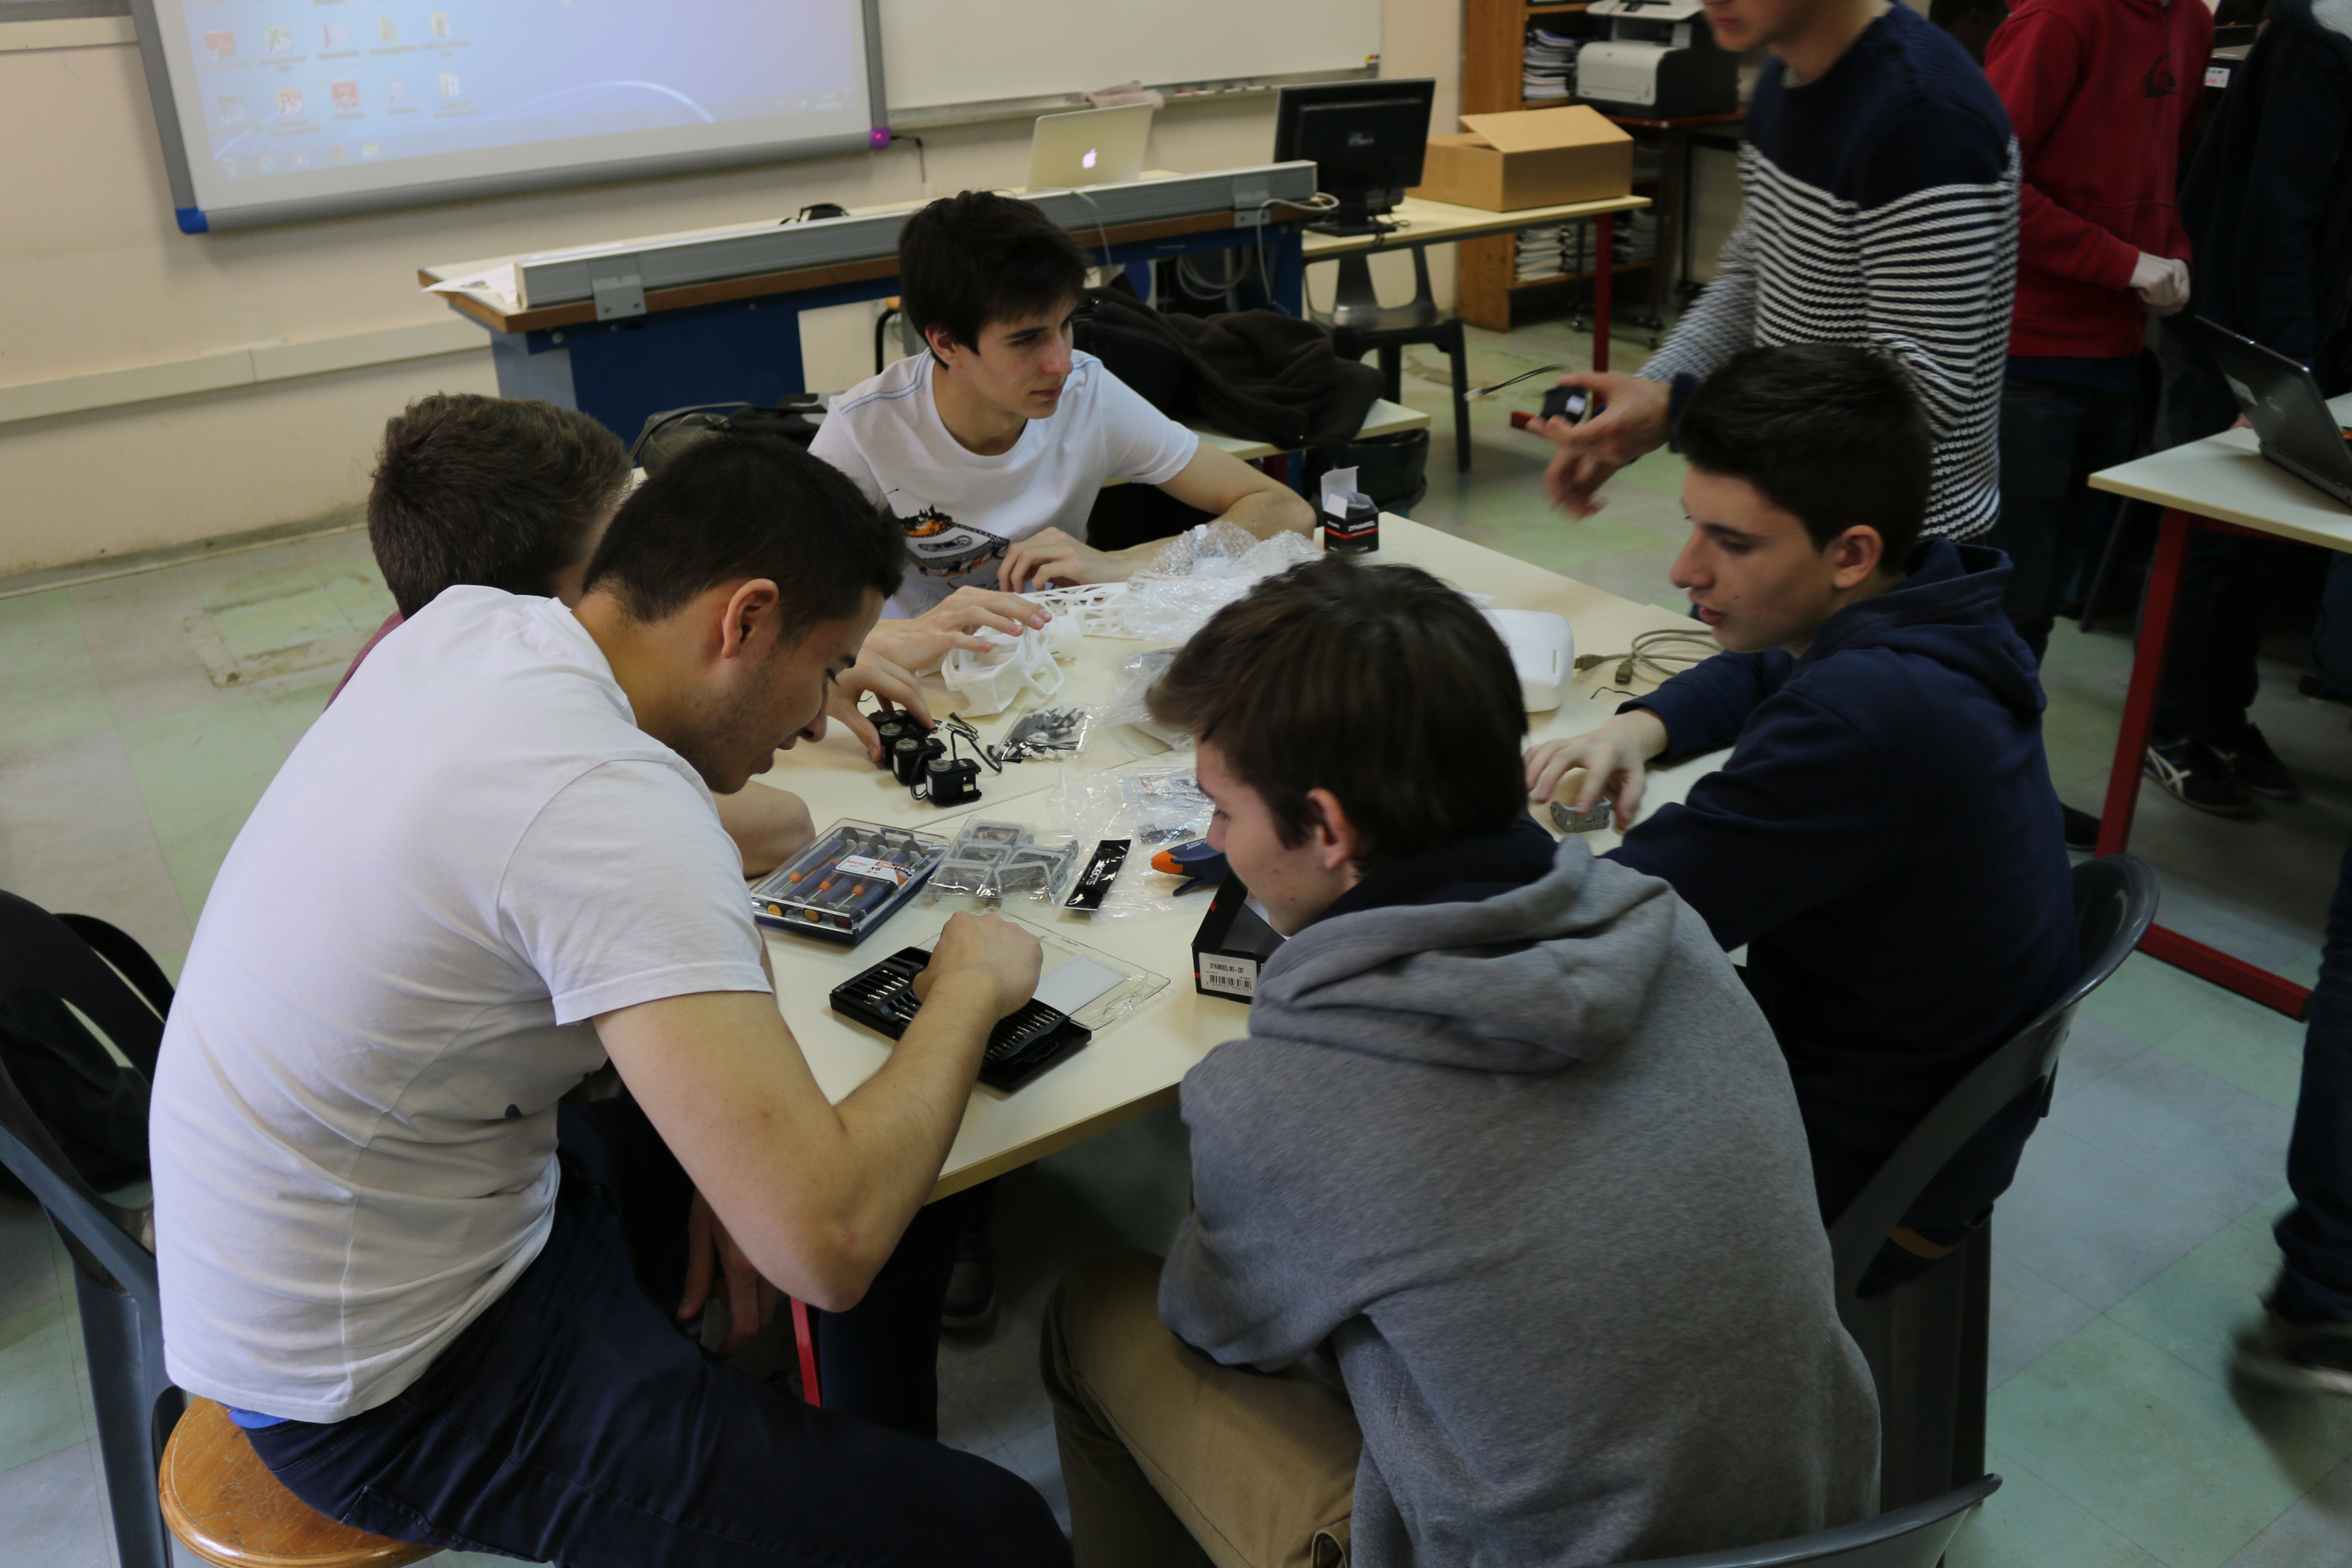
\includegraphics[height=4.4cm]{saintonge_assembly1.jpg}}
    \hfil
    \subfloat[][Thorax assembly]{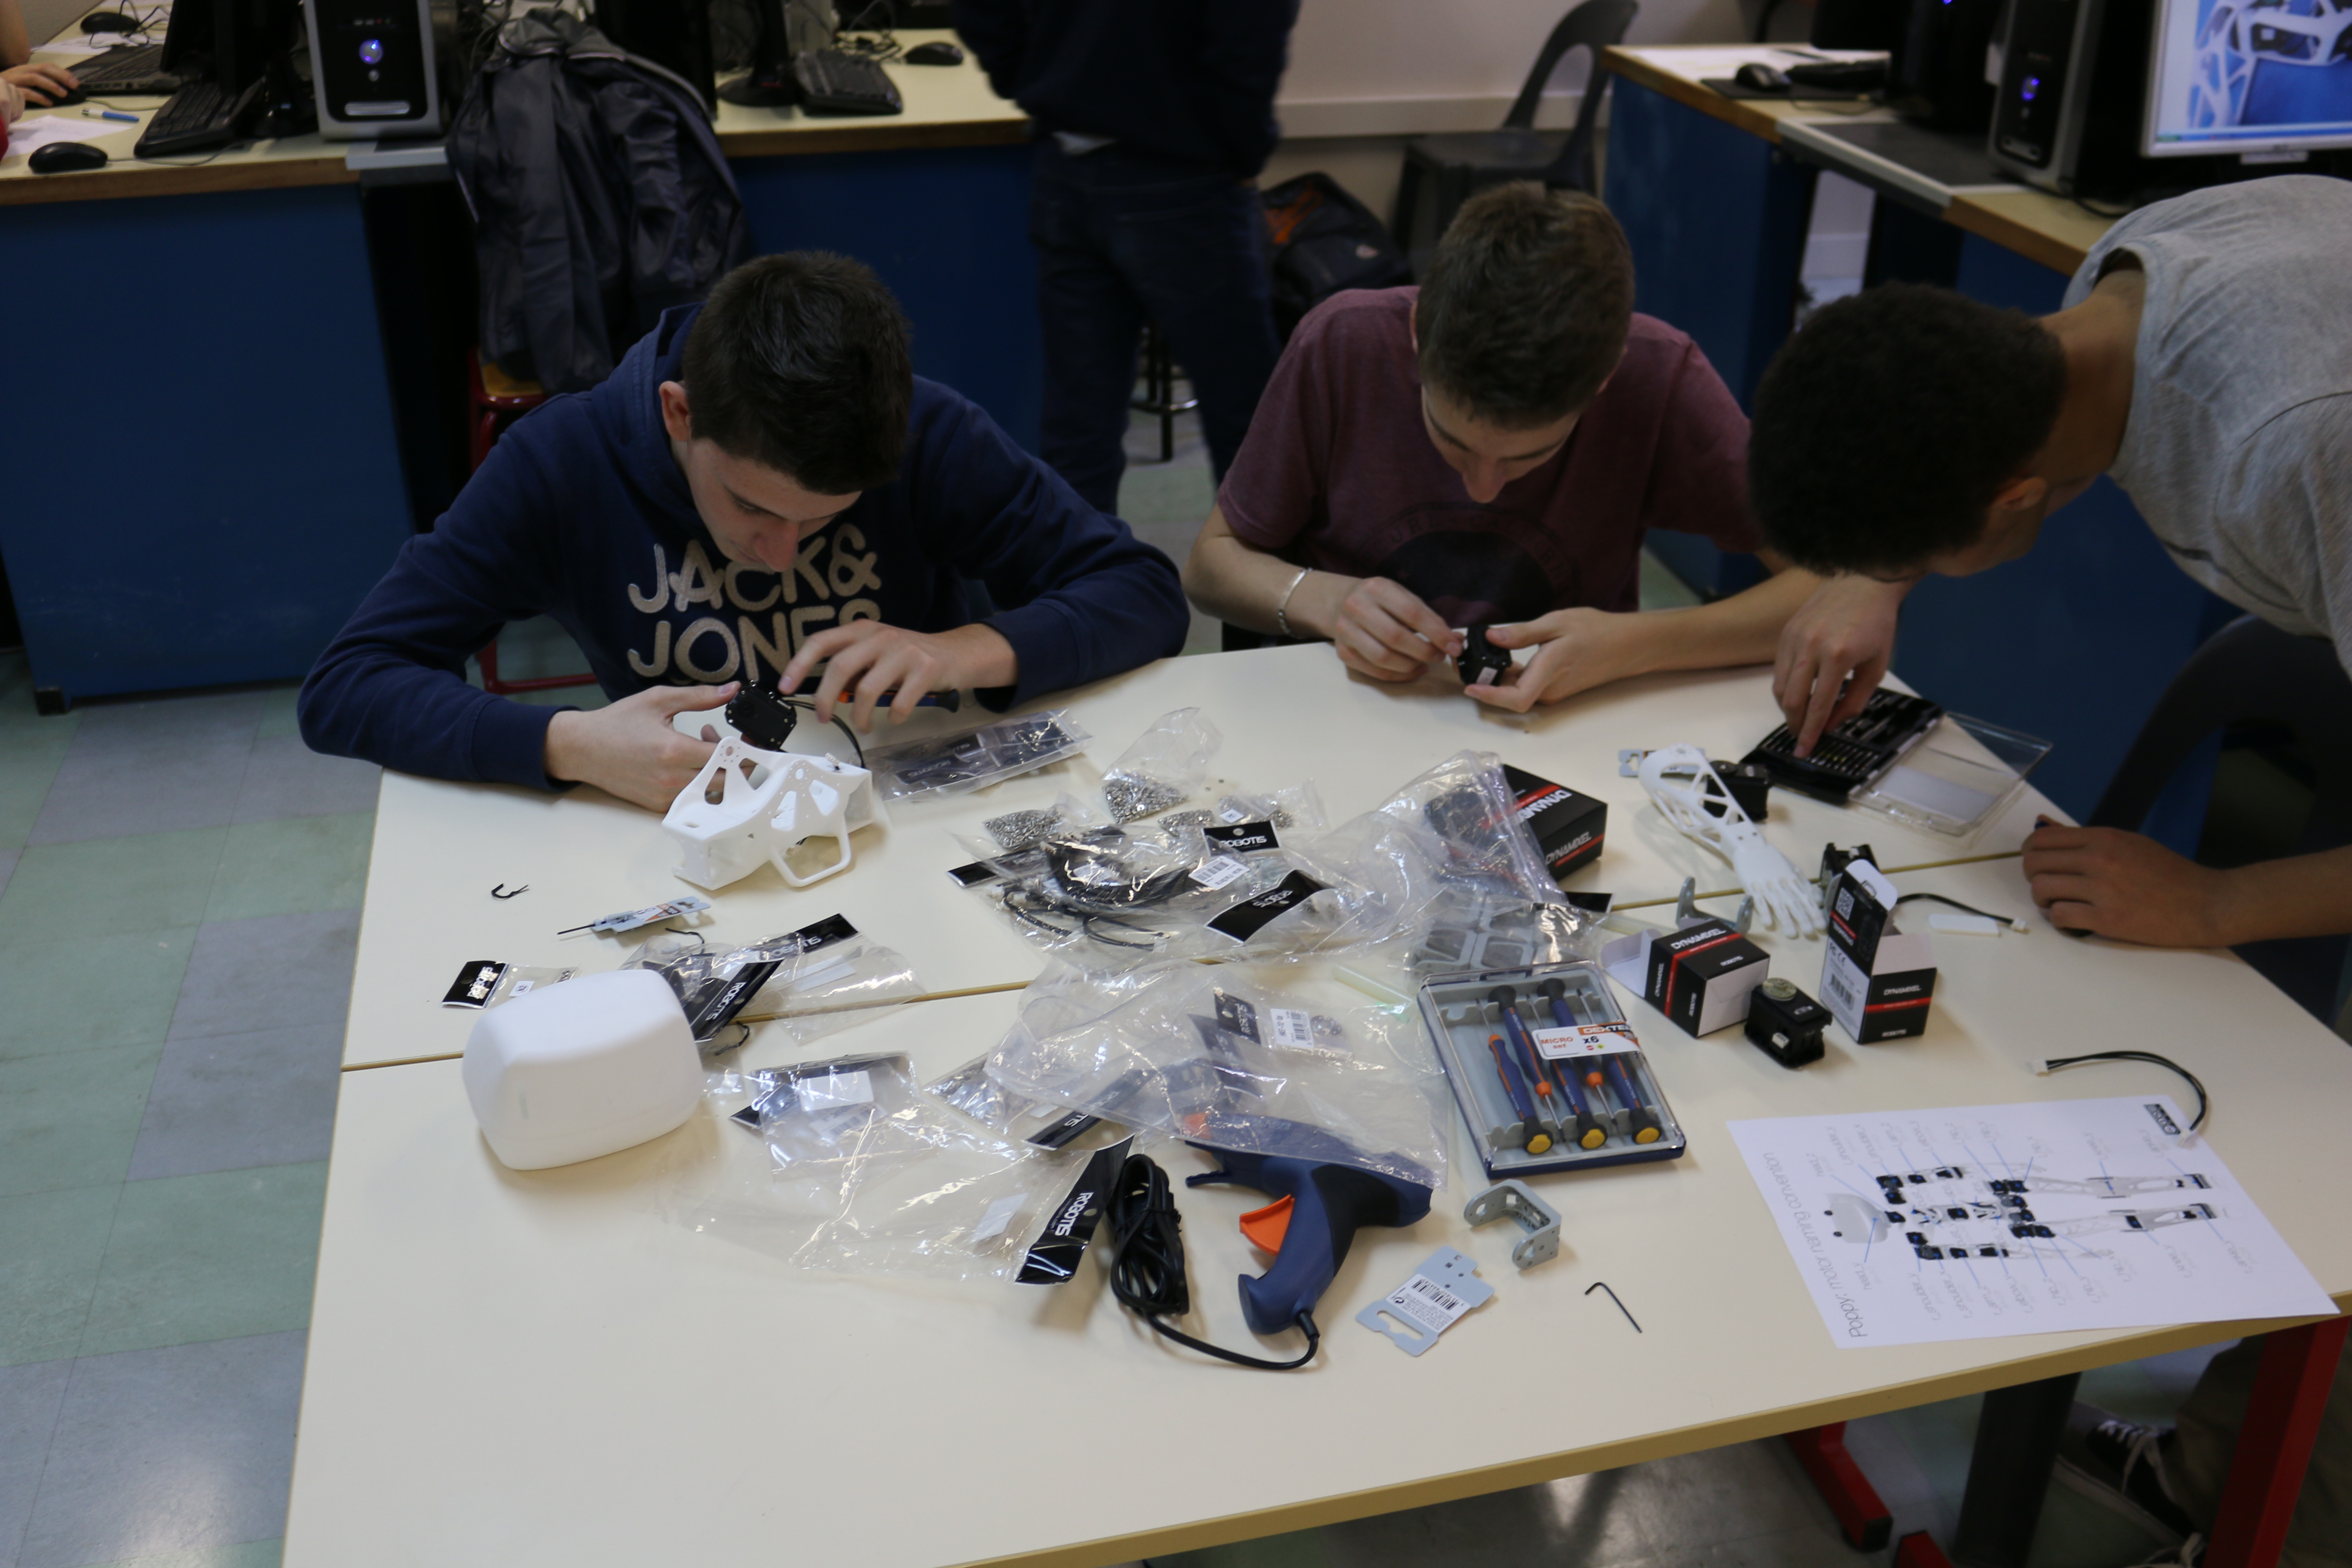
\includegraphics[height=4.4cm]{saintonge_assembly2.jpg}}
    \hfil
    \subfloat[][Arm assembly]{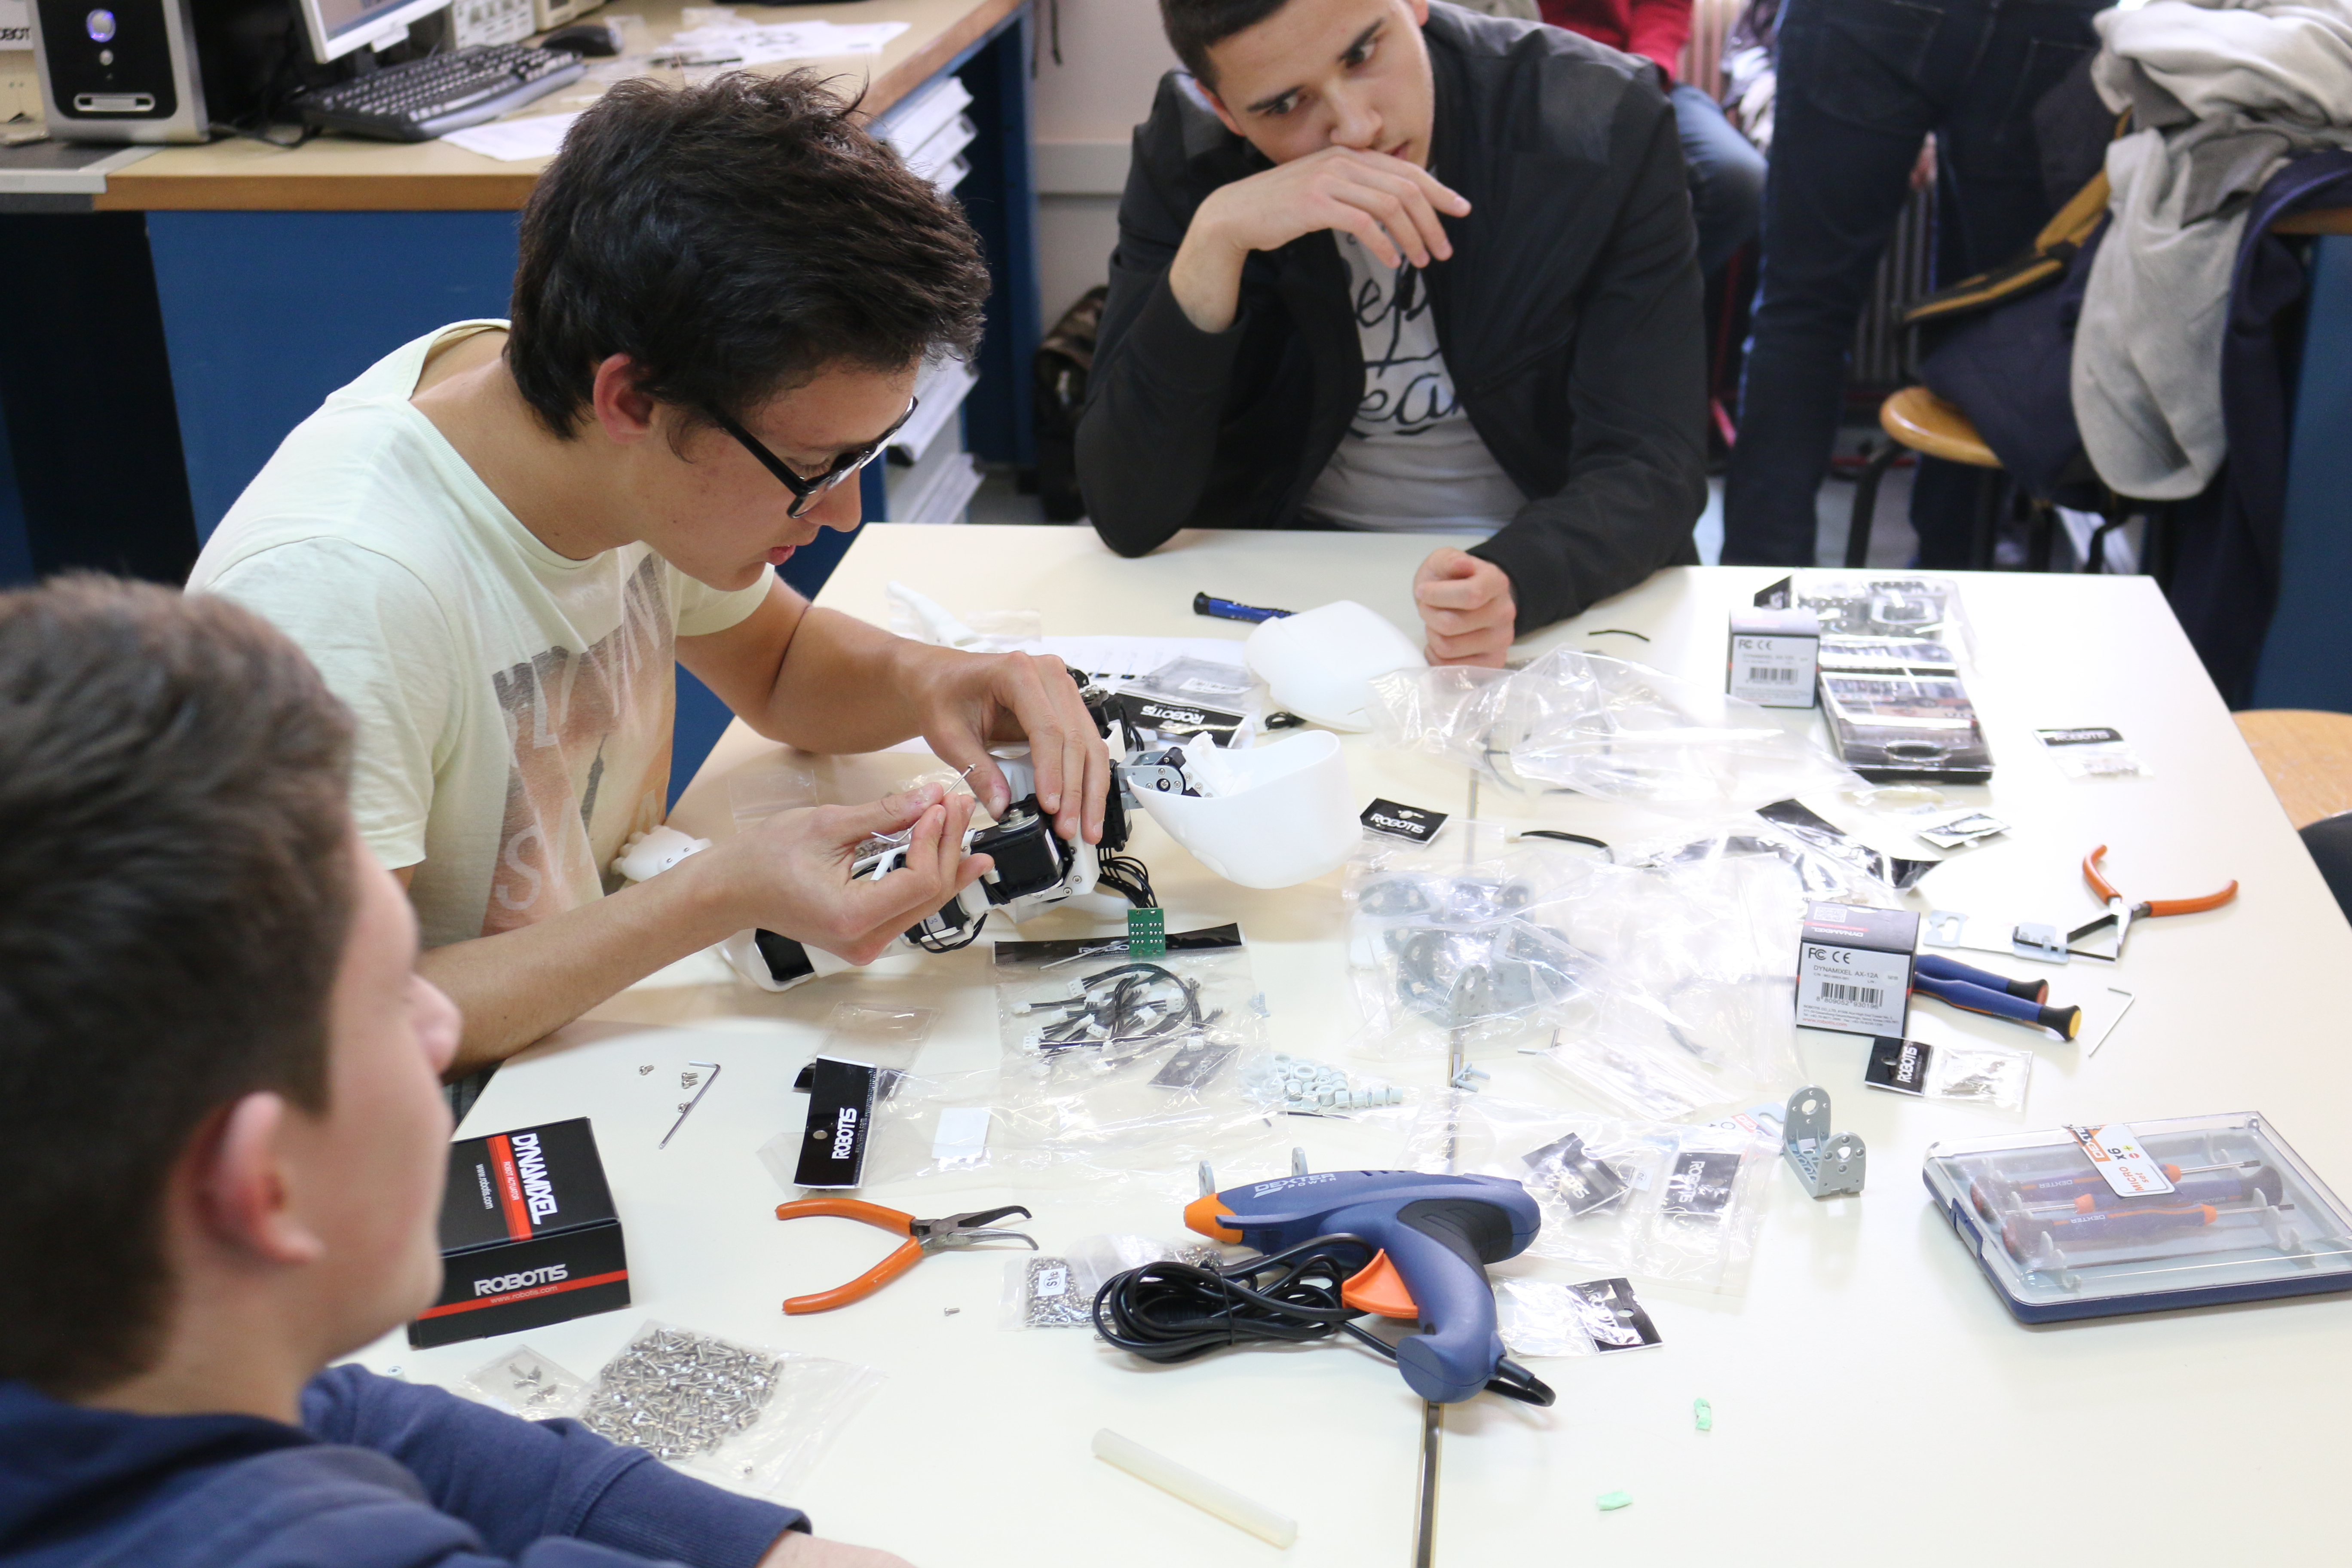
\includegraphics[height=4.4cm]{saintonge_assembly3.jpg}}
    \hfil
    \subfloat[][Poppy almost finished, only the face is missing]{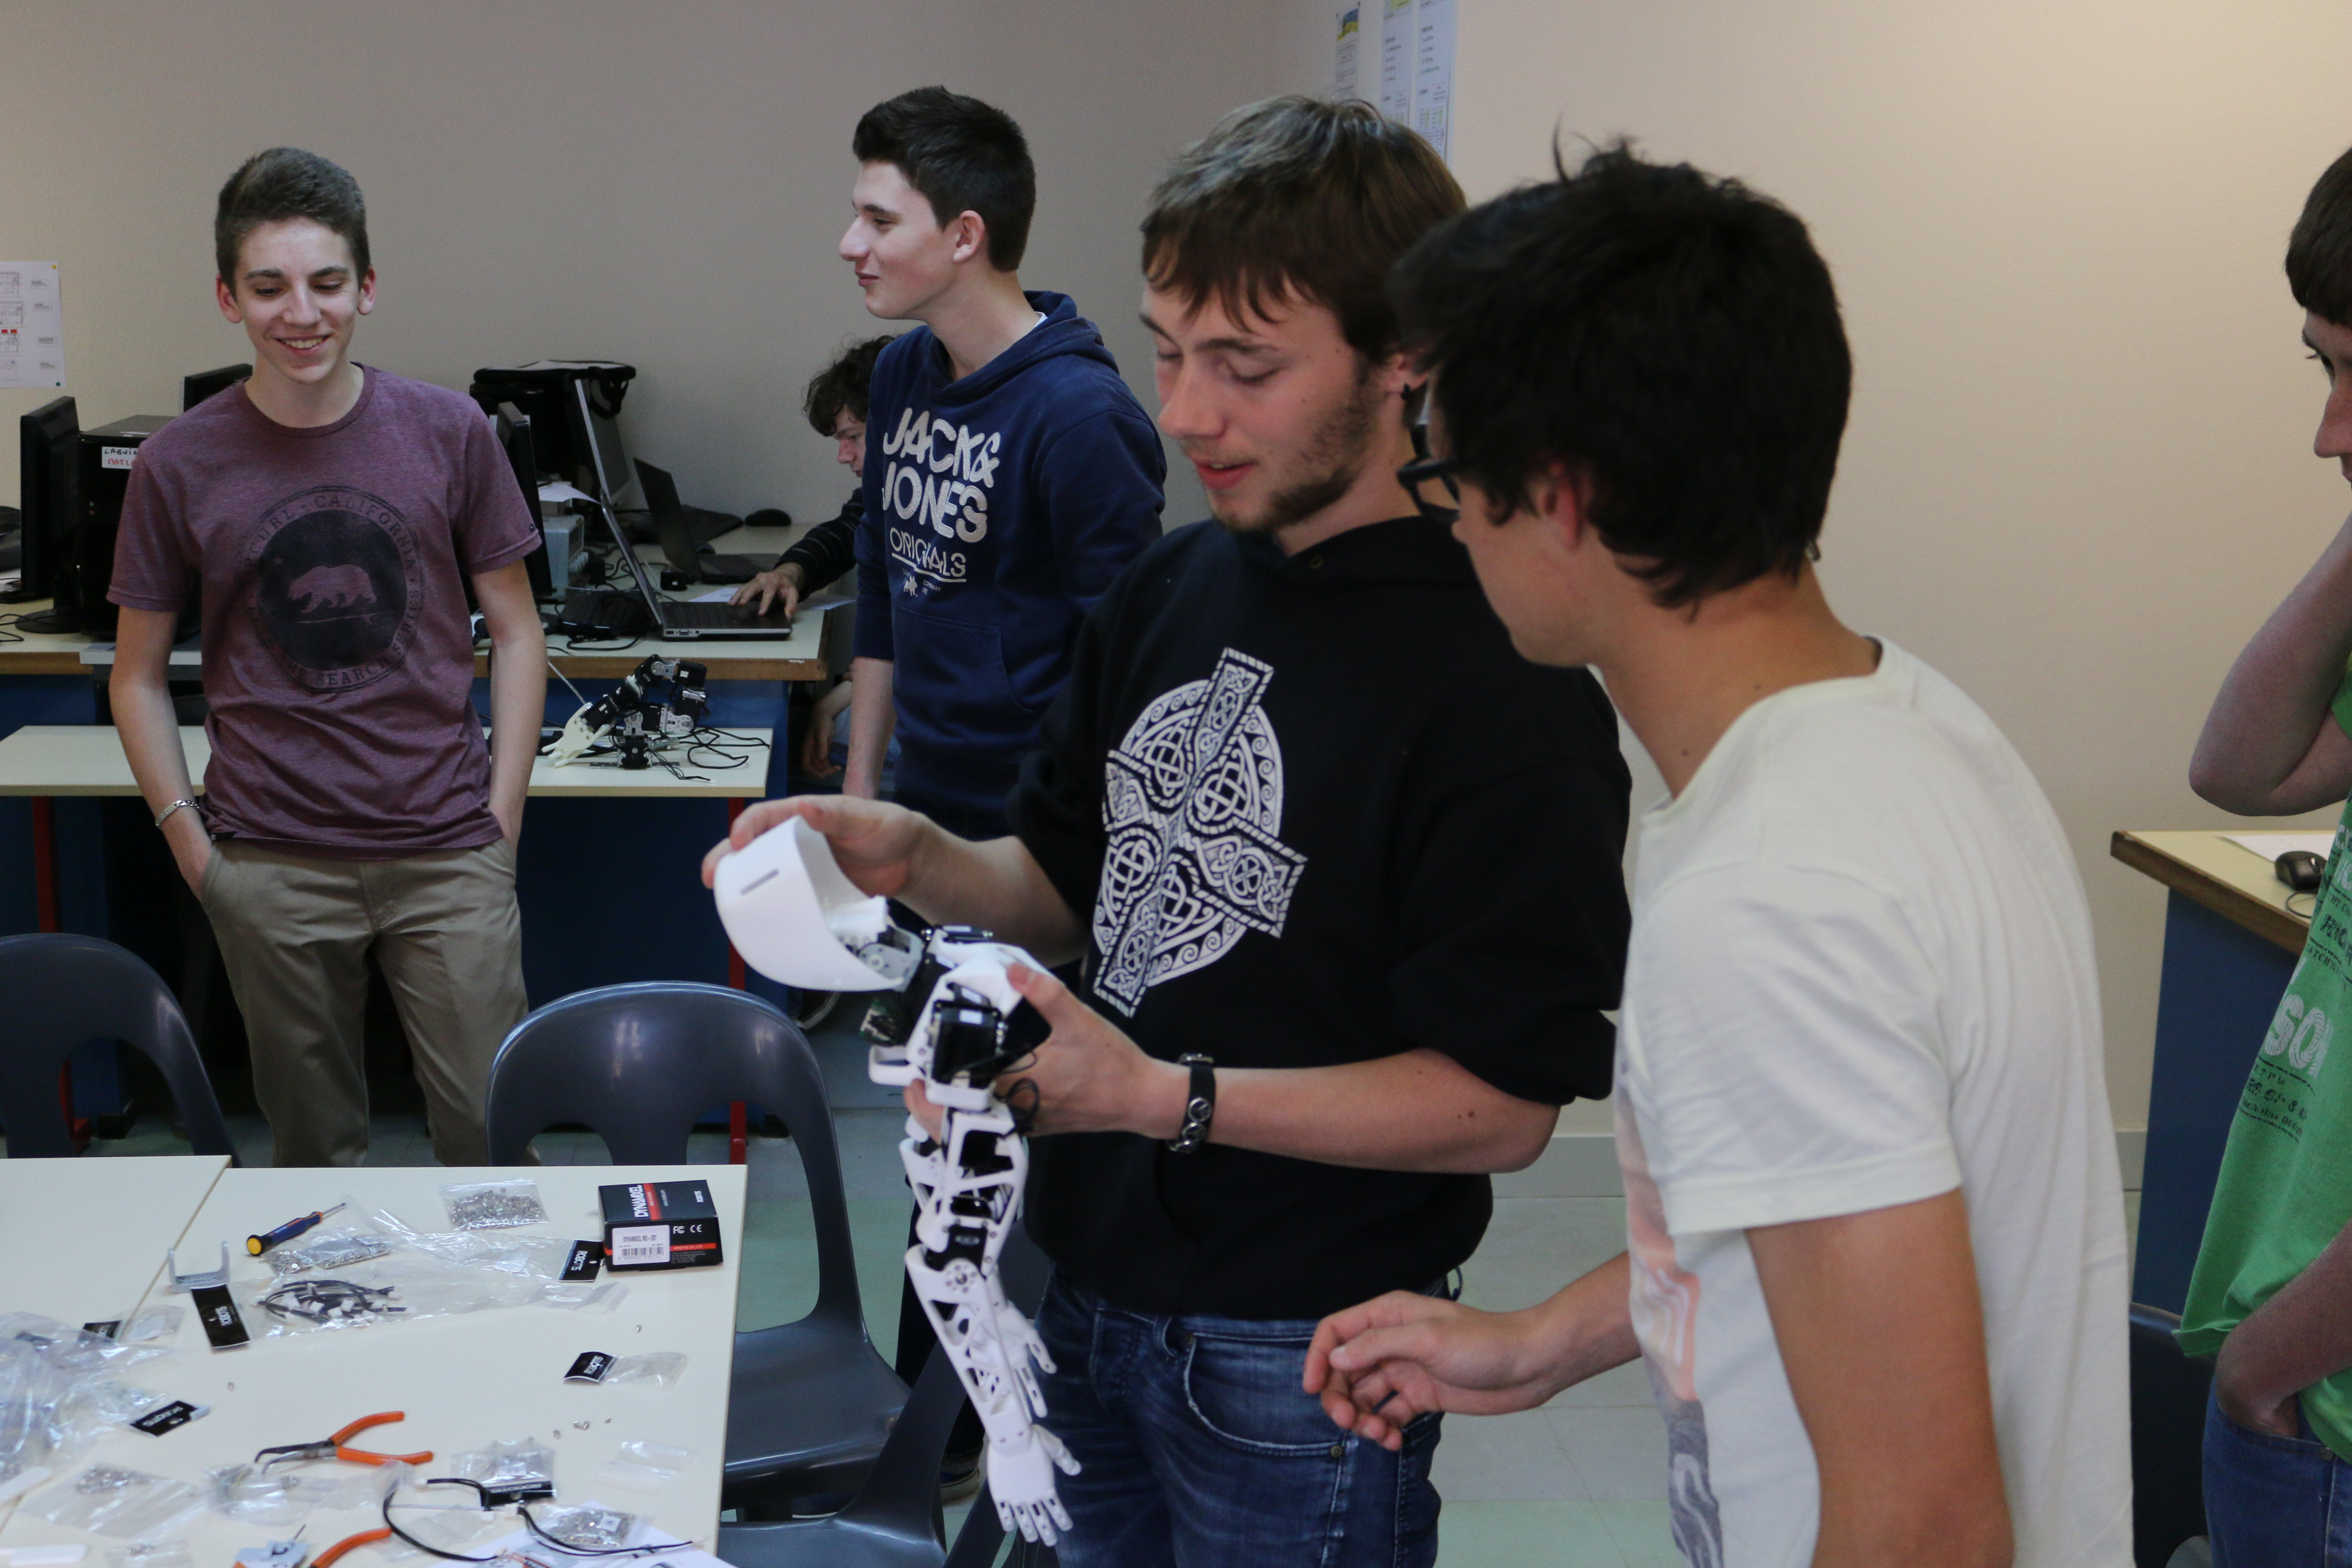
\includegraphics[height=4.4cm]{saintonge_assembly4.jpg}}
    \caption{Poppy was assembled by 3 parrallel working groups divided into thorax+head and the 2 arms. At the end of the first day, the half-Poppy was assembled and functionnal. }
    \label{fig:saintonge_assembly}
\end{figure}

However, as I will discuss with more detail in the futher section REF, we experienced some difficulties with high school internet connection and all documentation is online\dots So it was unfortunatelly a bit difficult to evaluate if our documentation was clear enough for high-schools student. Yet, from that I experienced explaining howto, we need a higlhy detailled documentation for the very first steps. Then general guidelines seem to be enough to achieve a well assembled Poppy robot.



\subsubsection{Python programmation with pypot}

Two working groups were dedicated to learning basic Python and programming with pypot (see \figurename~\ref{fig:saintonge_software}). The teacher has selected these students because of their computer science enthousiasm. Indeed when they heard about the Poppy project few weeks ago, they got interested by Python and began to look for futher information on internet.

The first hours of the software workshop have been complicated. The school computers were not outdated but were under windows and used by a lot of different people, so configurations were not consistent between machines. The installation of the necessary tools (Python + packages + texte editor) has been really long and painfull. I will come back to this point in the section REF.

Once desktop were setup, students took a look to the basic pypot tutorials. They first tried to control one dynamixel motor (reading/setting positions). Then they use a group of motors (each having one Poppy arm) and we introduce the pypot robot configuration file. At this point they were able thanks to the basic pypot tutorial to create a robot with specific motor configuration and make it move using direct goal position or using sinus trajectories.

This improvised complexity slope leads them to a well understanding of the very basic features of pypot and Dynamixel motor properties in just 2 hours and without any Python experience.

Then the hardware groups get Poppy assembly done, the software group modified the Poppy's configuration file and adapted it to their own Poppy. At the end of the first day, the two groups were able to make their Poppy move.

The software guys continued their work the next day, trying to create more complex behavior. One of them (see \figurename~\ref{fig:saintonge_motivated_software_guy}), managed to create on his own (I did not write any line of code) the copy-arm behavior we showed in the Poppy overview video\footnote{http://vimeo.com/poppyproject/poppyoverview}. Then he explained how he did it to his classmates (see \figurename~\ref{fig:saintonge_knowledge_transmission}).

After learning how this behavior was done, another group decided to make Poppy clap its hands. By trial-error they manage to make the basic motion using sinus. This self-exploration raises the need to understand what is a variable, how a sinus acts and they experimented by their own the different sinus properties such as frequency, amplitude and even offset.

As Mitchel Resnick explained in REF, here the meaningful context of making a robot move leads students to be curious about mathematics and computer science concepts.


\begin{figure}[]
\centering
    \subfloat[][One software working group discussing pypot with their teacher]{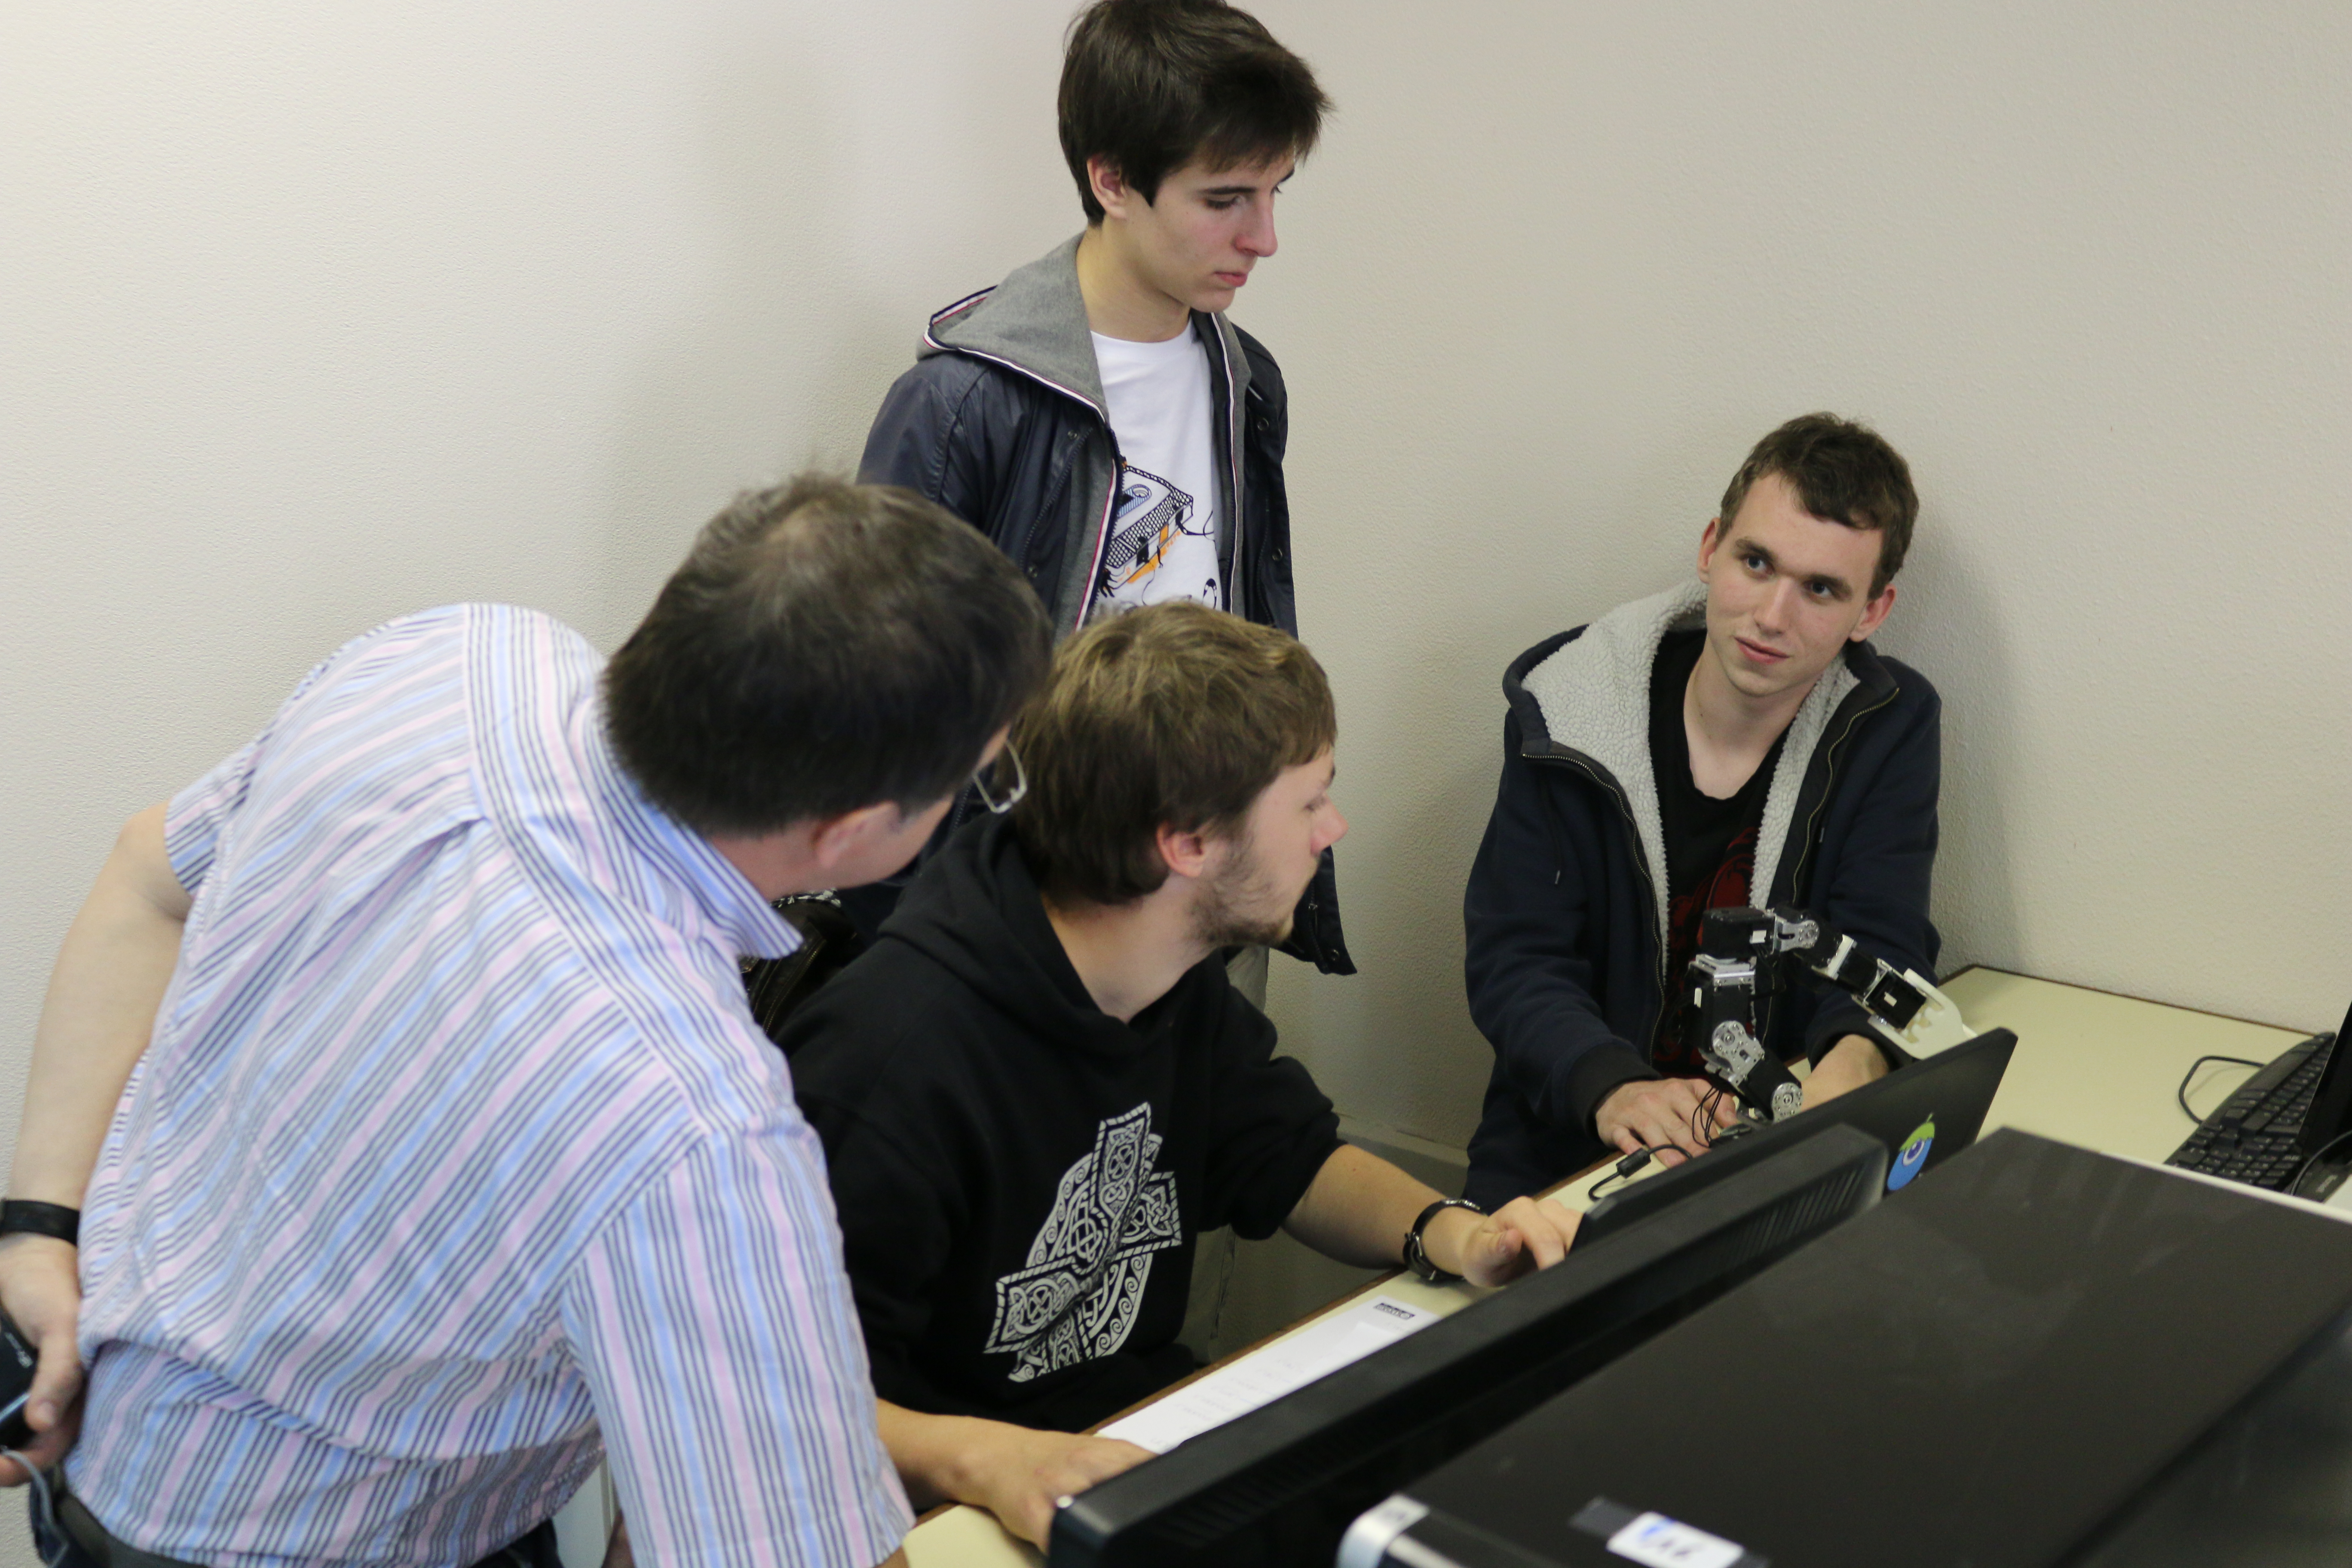
\includegraphics[height=4.4cm]{saintonge_soft1.jpg}}
    \hfil
    \subfloat[][The two software groups discussing about Poppy's configuration file]{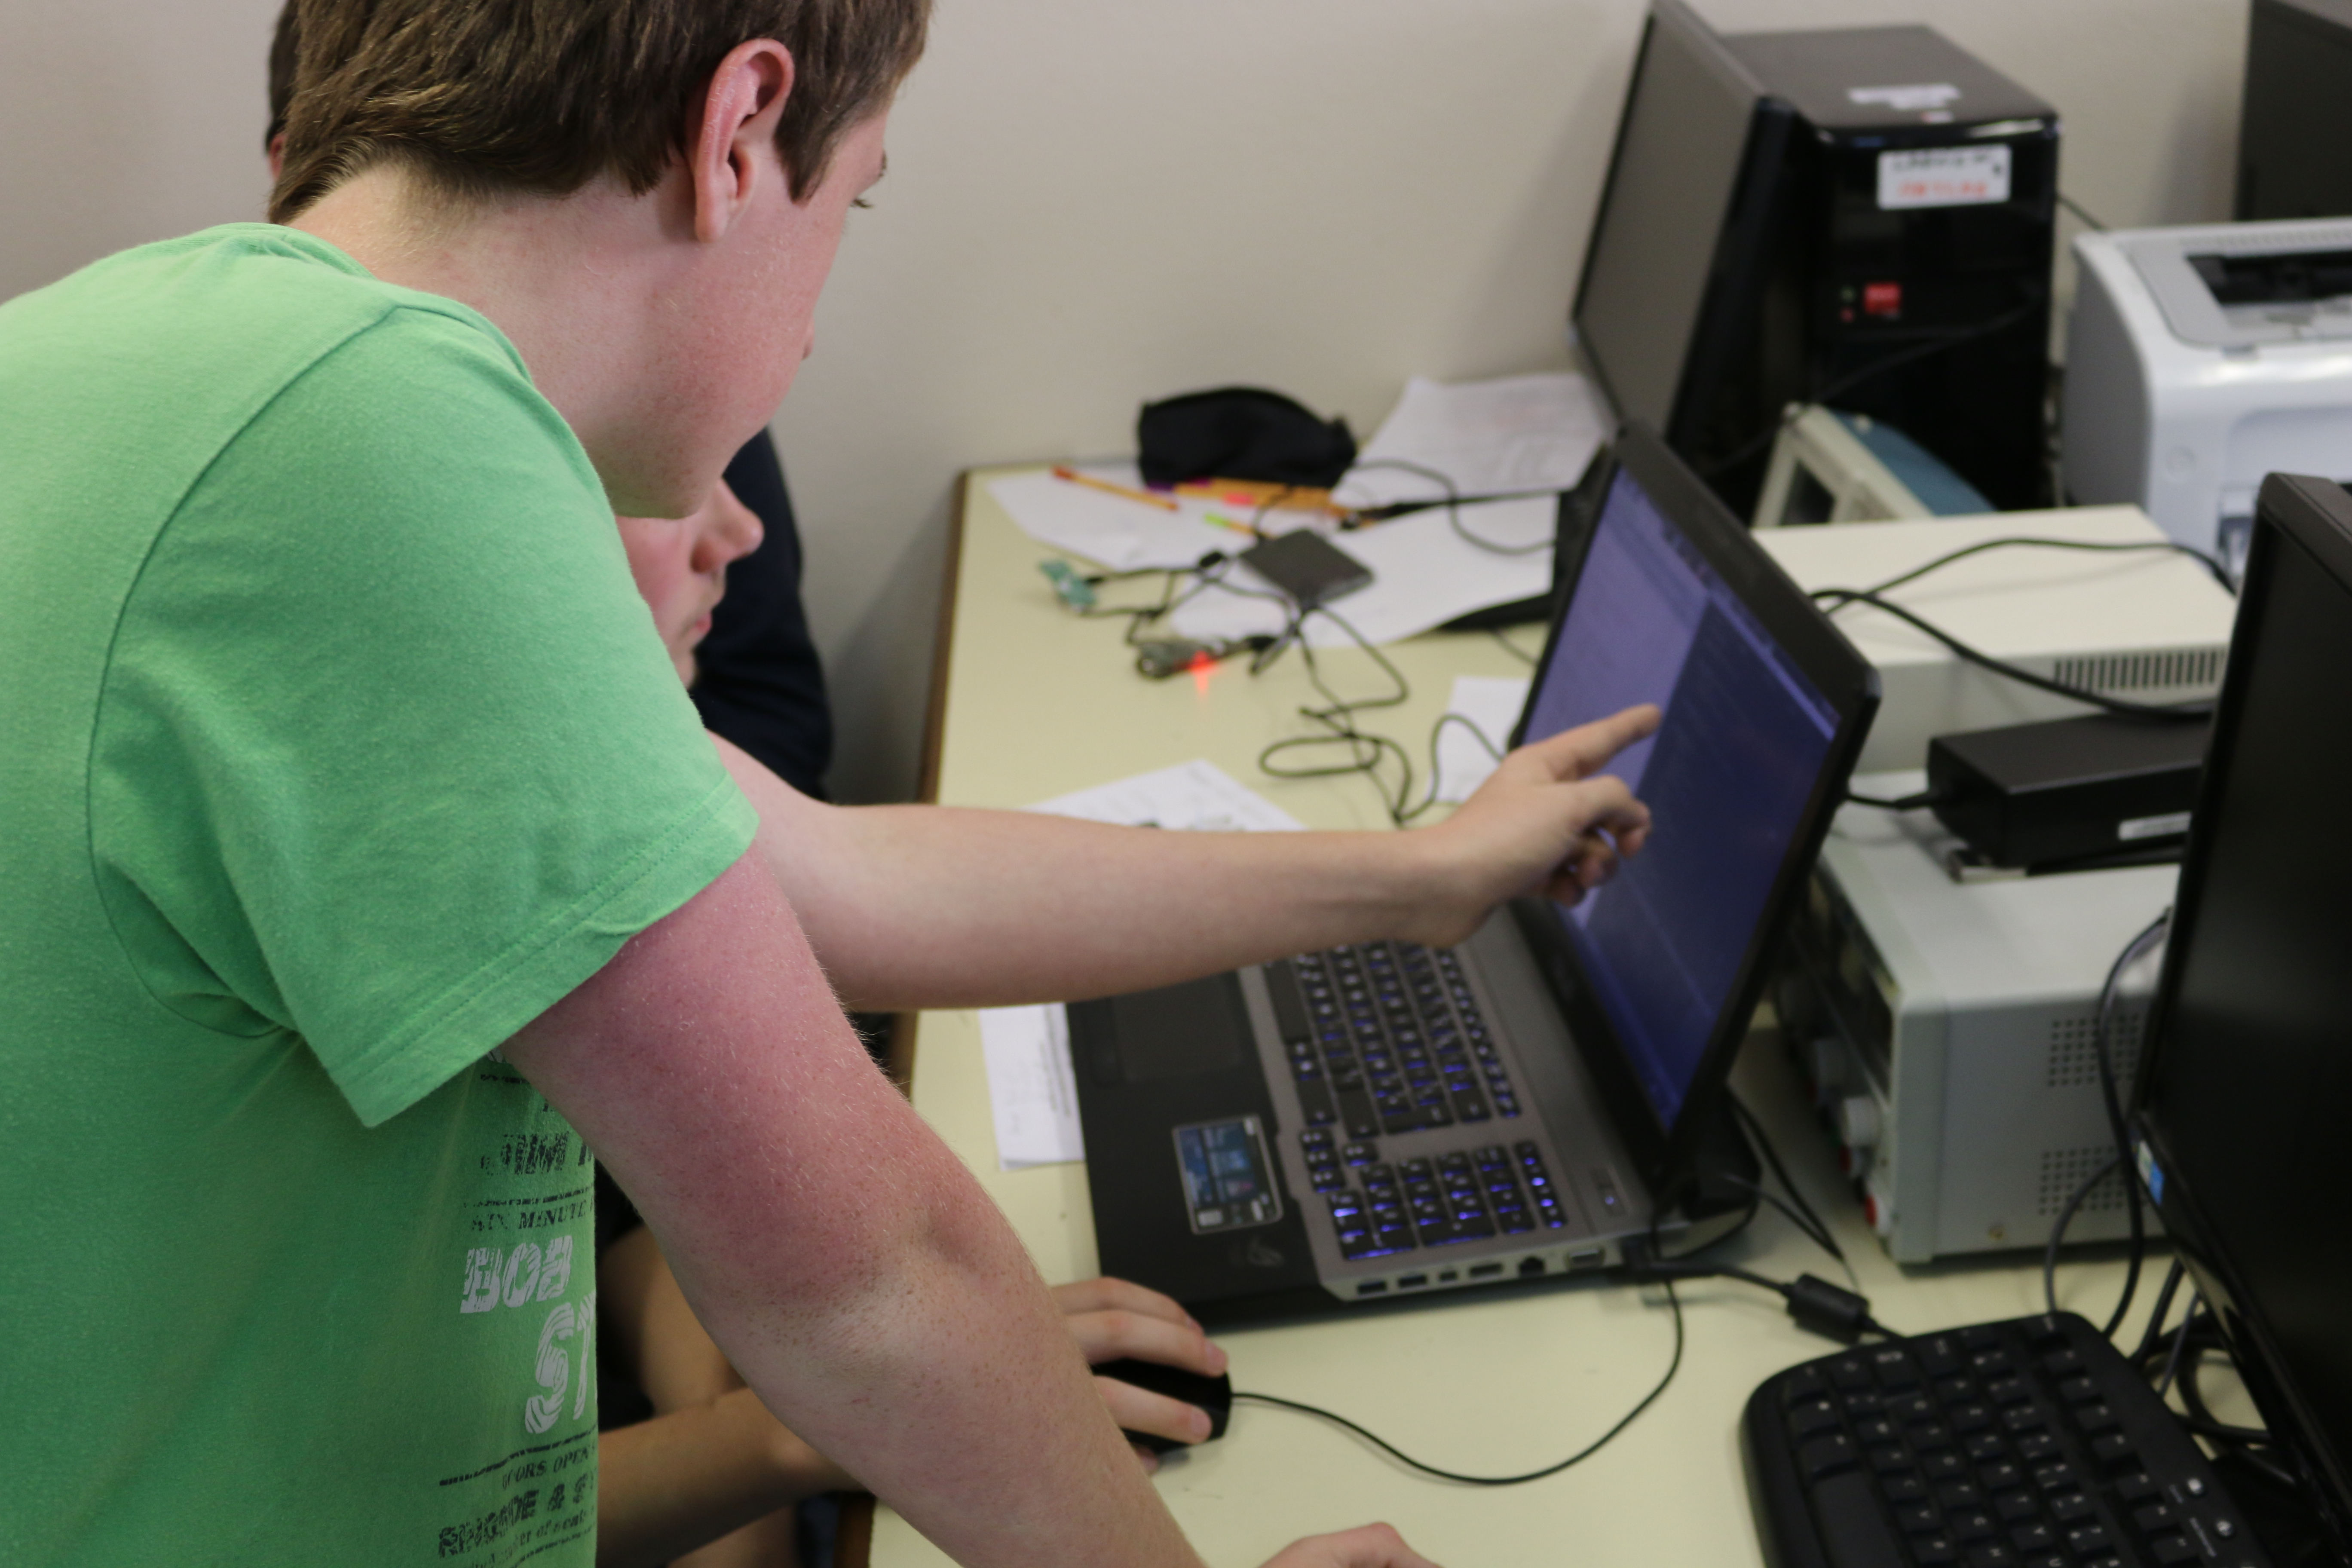
\includegraphics[height=4.4cm]{saintonge_soft2.jpg}}
    \hfil
    \subfloat[][Experimentation trough trial-error]{\label{fig:saintonge_motivated_software_guy}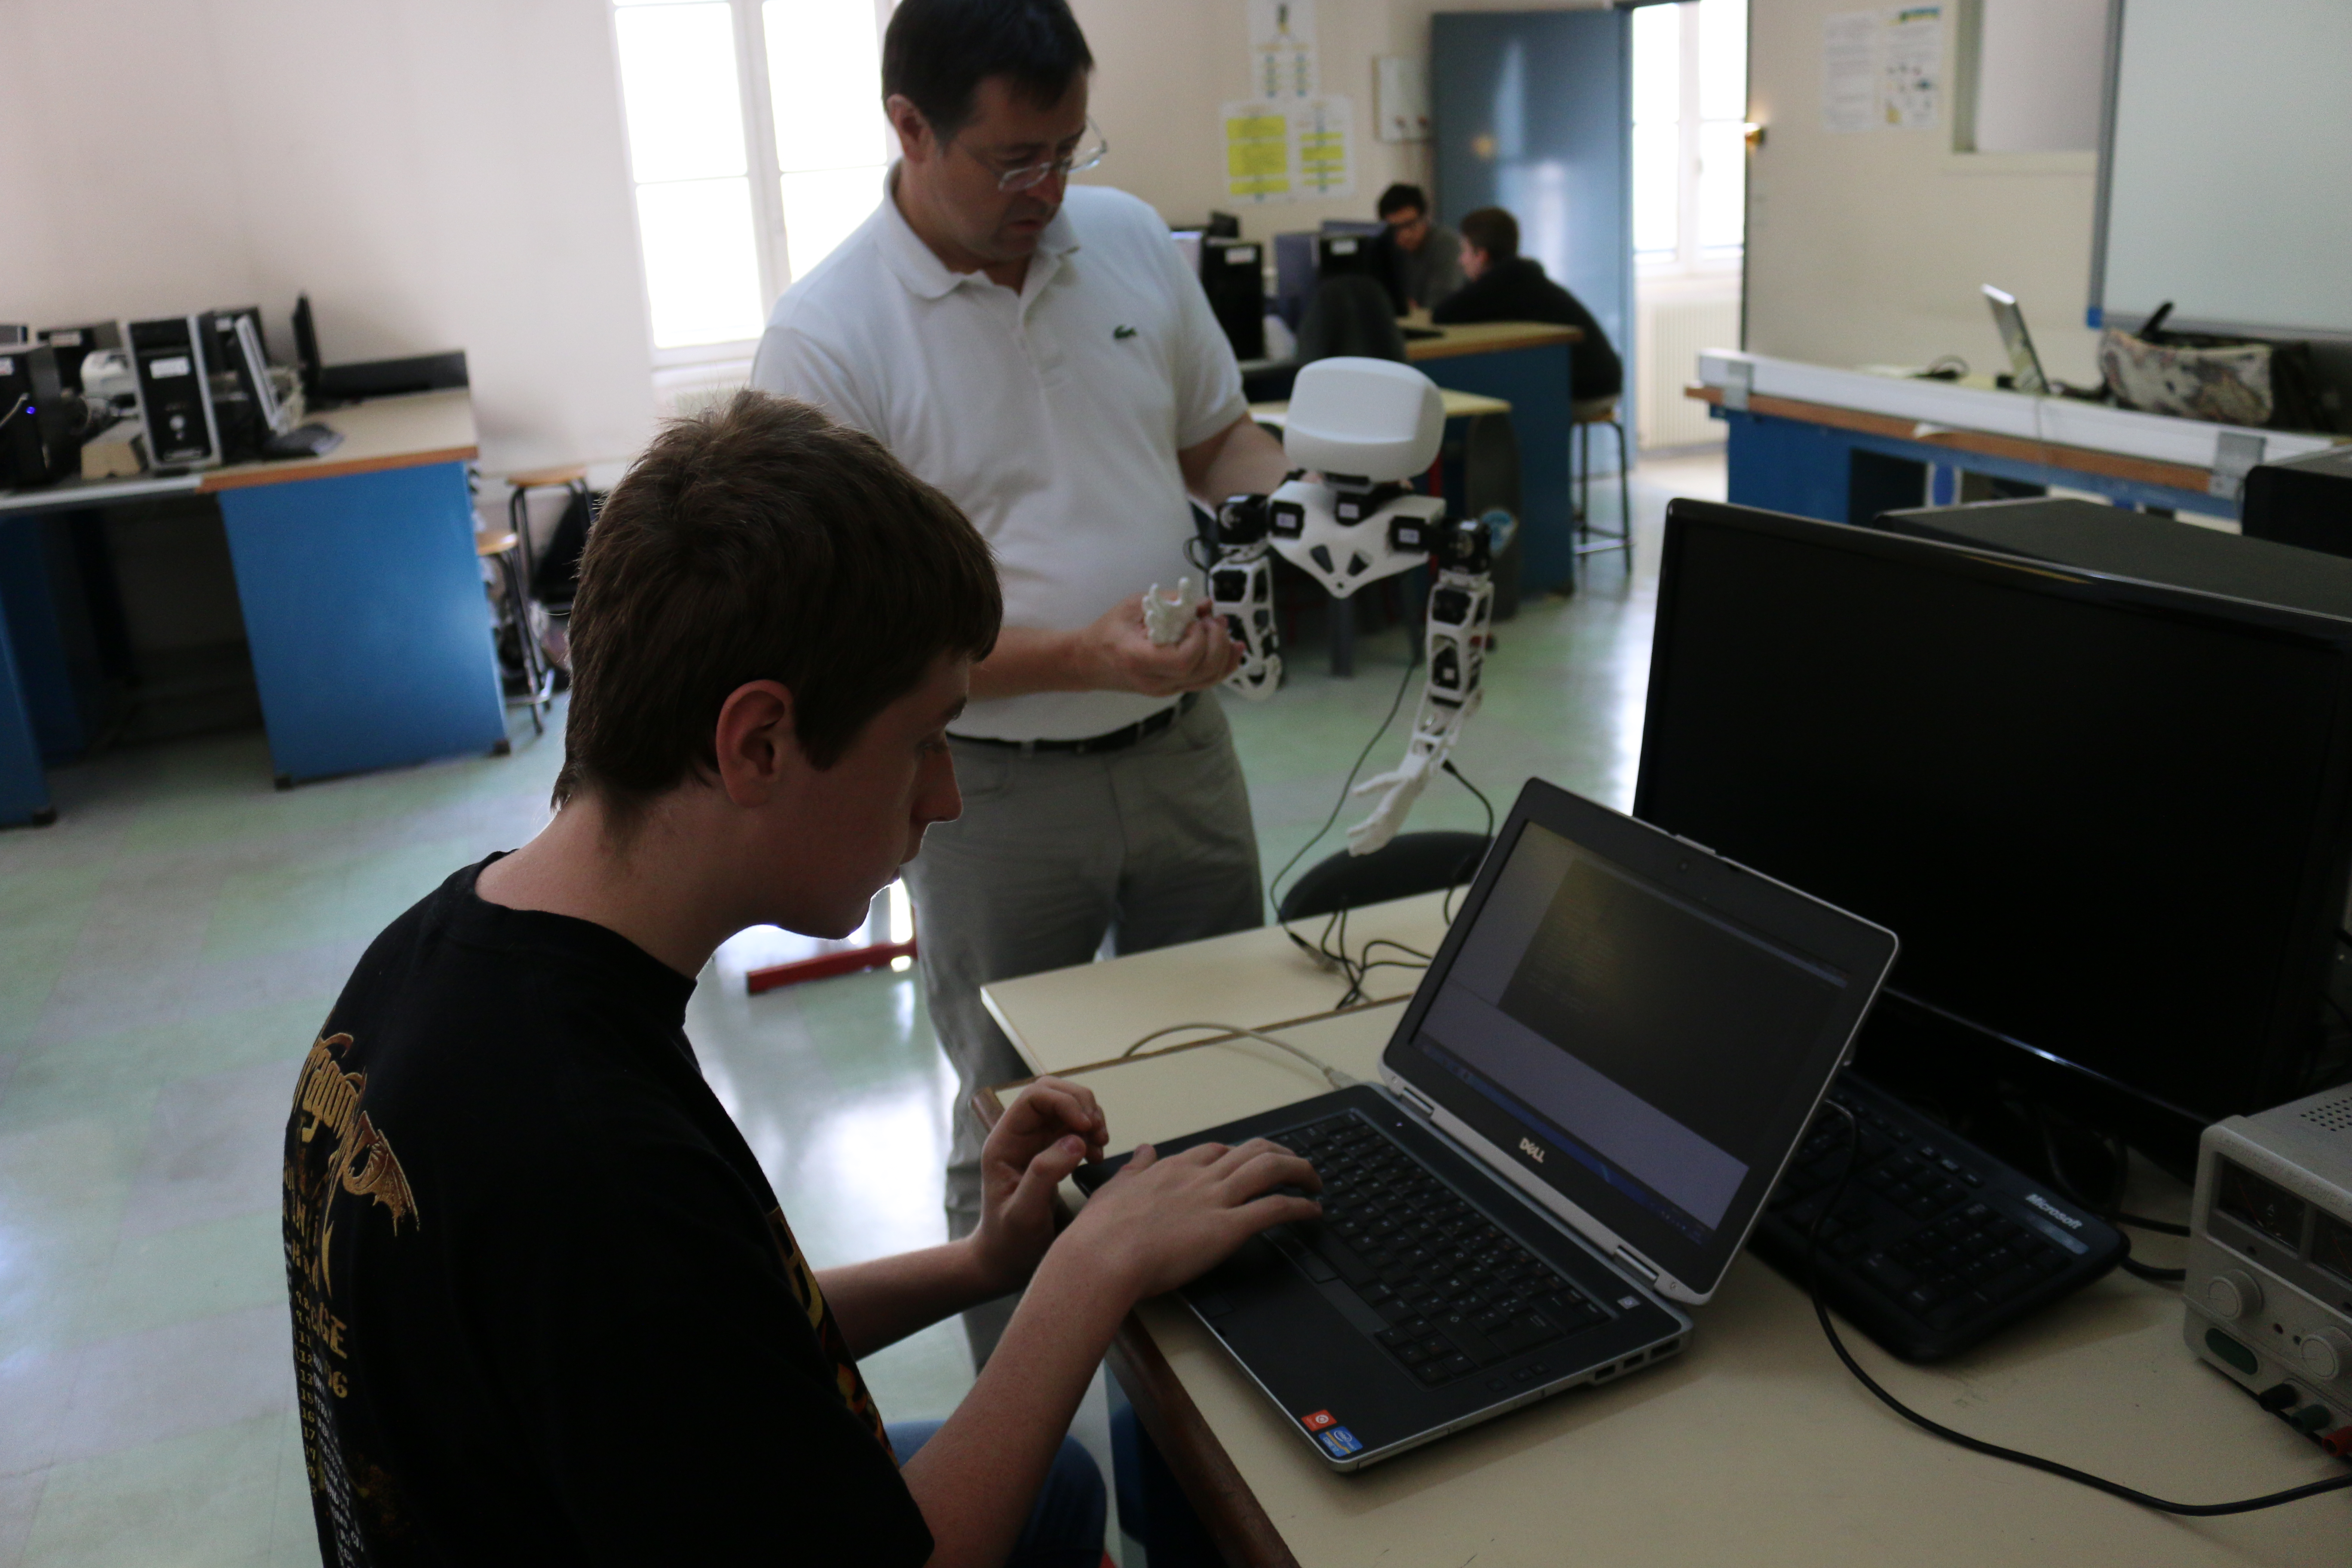
\includegraphics[height=4.4cm]{saintonge_soft3.jpg}}
    \hfil
    \subfloat[][Transmission of knowledge between classmates]{\label{fig:saintonge_knowledge_transmission}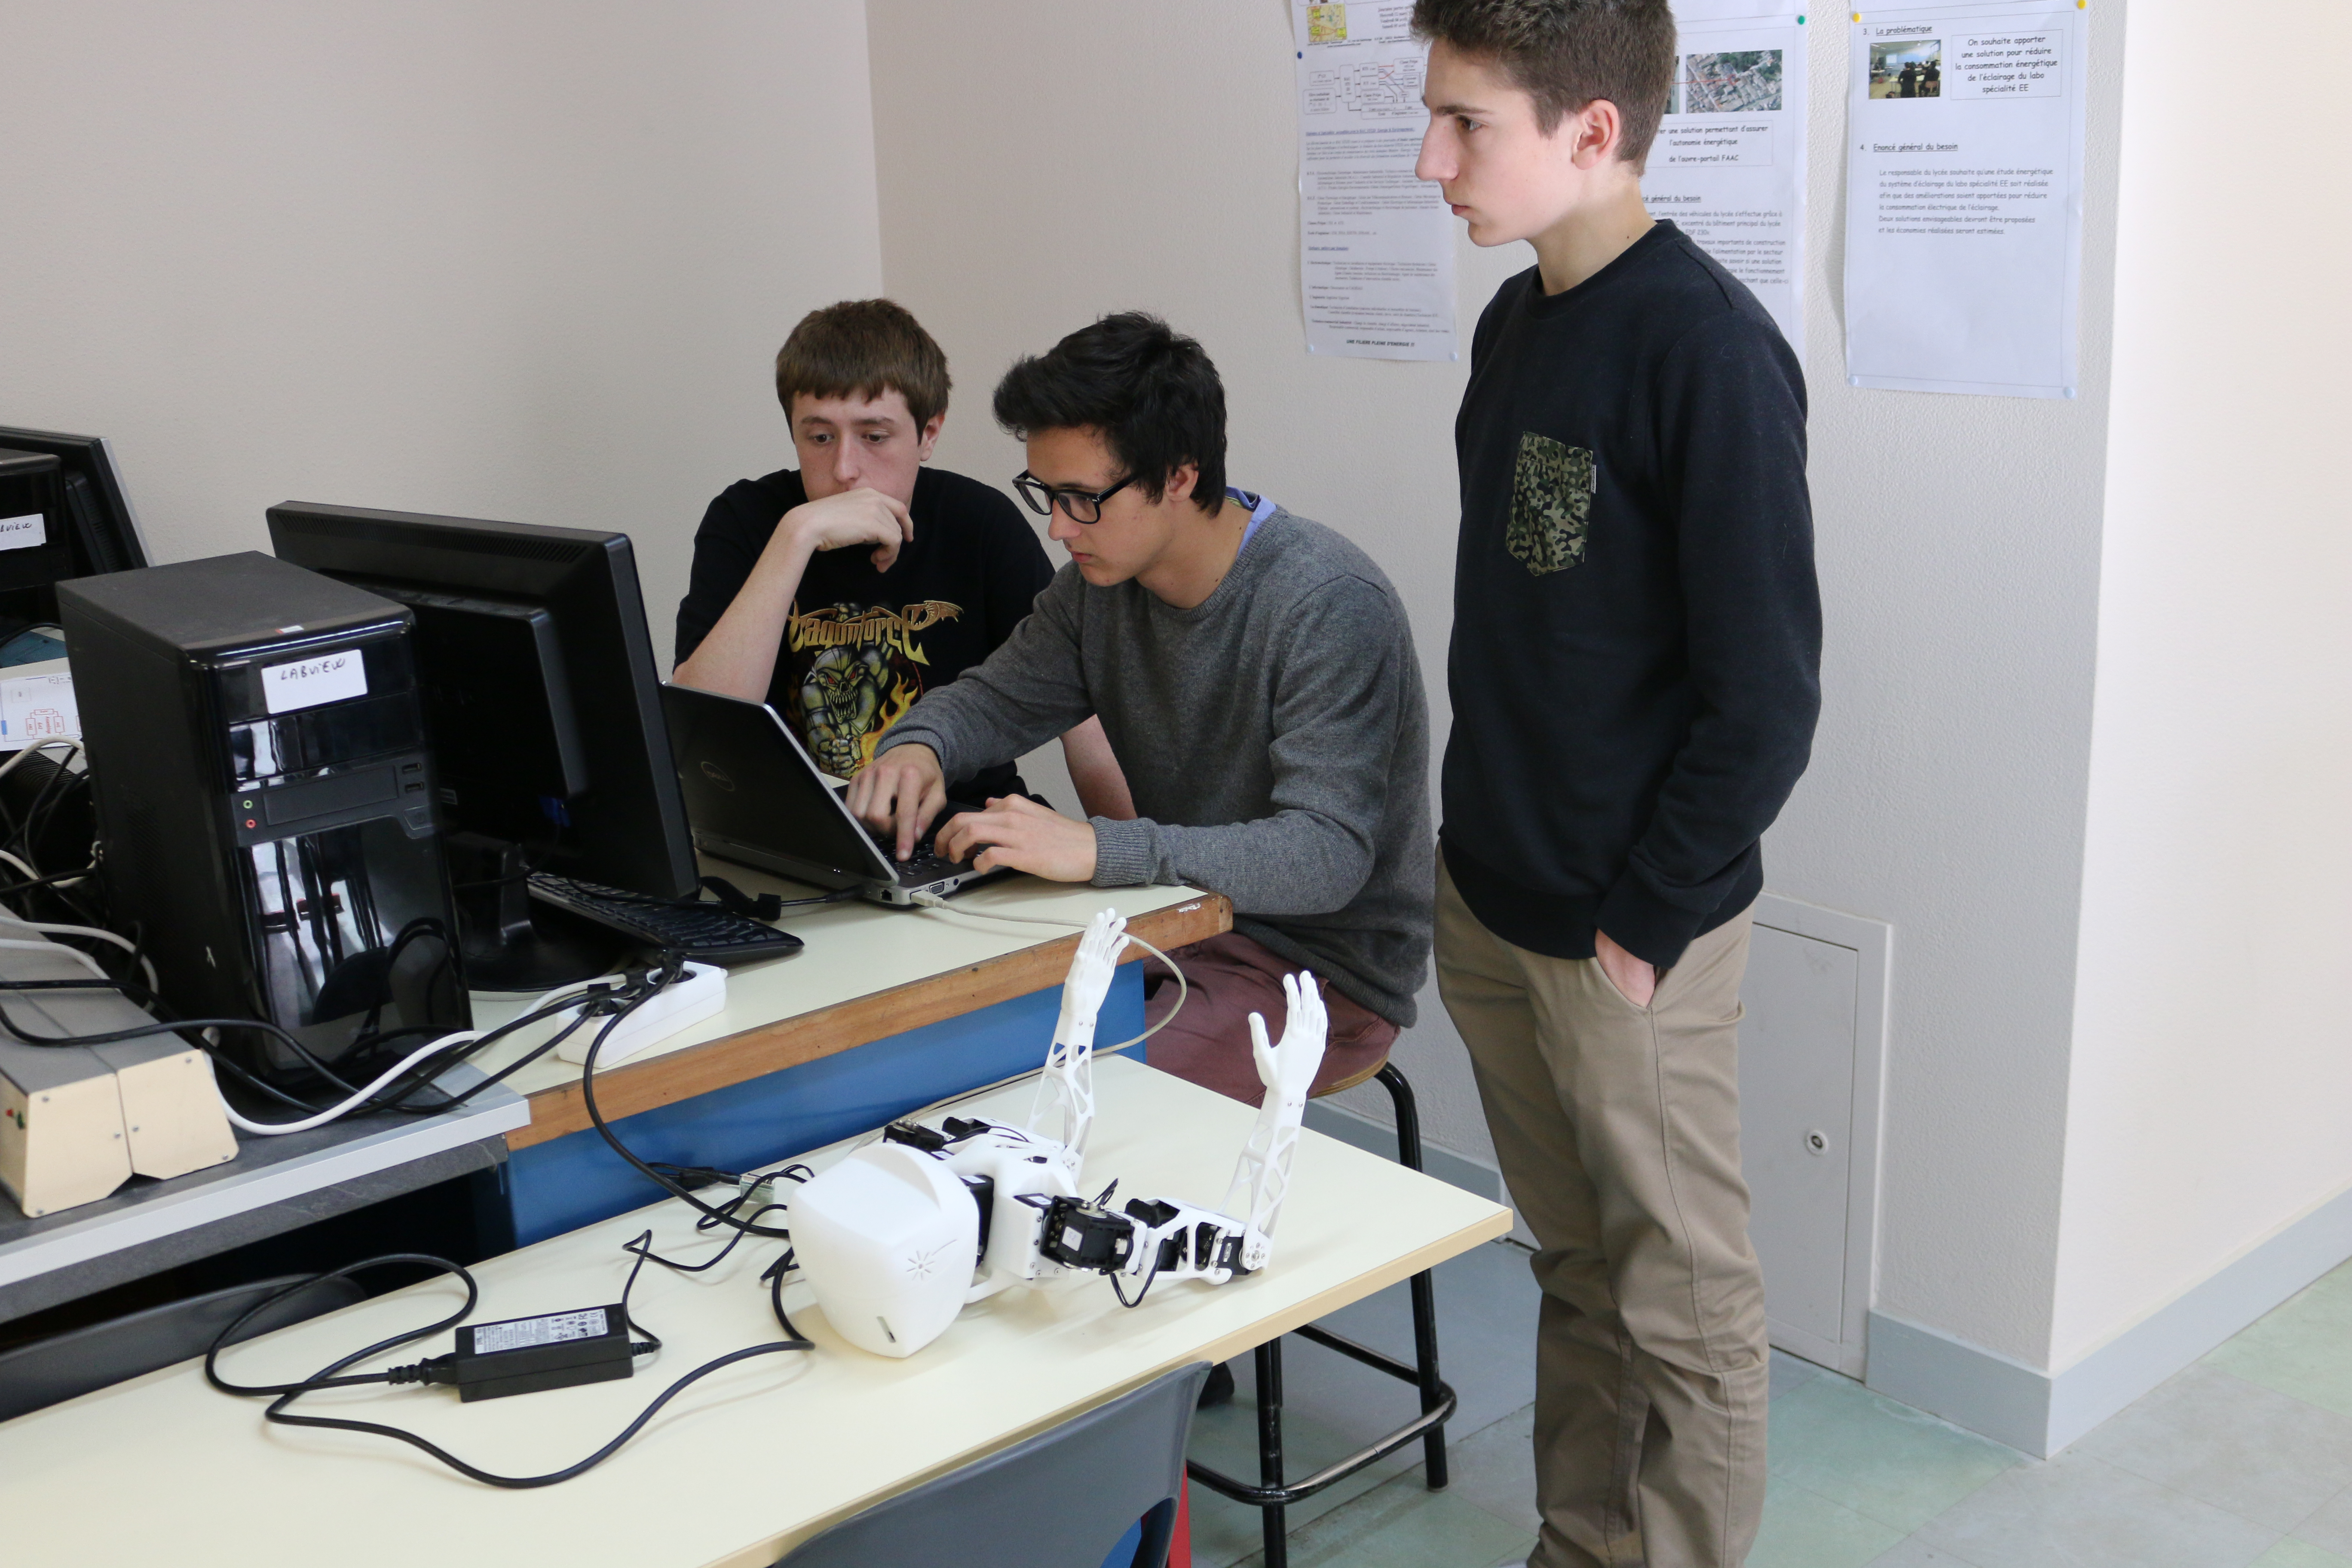
\includegraphics[height=4.4cm]{saintonge_soft4.jpg}}
    \caption{High-school students discovering programmation with Python and the pypot librairie}
    \label{fig:saintonge_software}
\end{figure}

\subsubsection{Design of a Poppy's support in Solidworks} % (fold)

As we was only builing the very upper part of the robot, several students worked in pair to design wheeled platform supporting their Poppy version. The teacher instructions was to create a mobile support for their Poppy with enough room to include batteries and a computer.

For most of them it was the first introduction with the use of parametric modeling tools. However, the final result (see \figurename~\ref{fig:saintonge_support}) is quite impressive. All working pair managed to finish the design of the basic idea of their conception choice and integrate the Poppy robot.

A really interesting point is the fact they all choose a differente conception to make their support move. Some used carterpillar, other four wheel or two and a free wheel. The Poppy robot give a pretext to creation.

\begin{figure}[]
\centering
    \subfloat[][Caterpillar design]{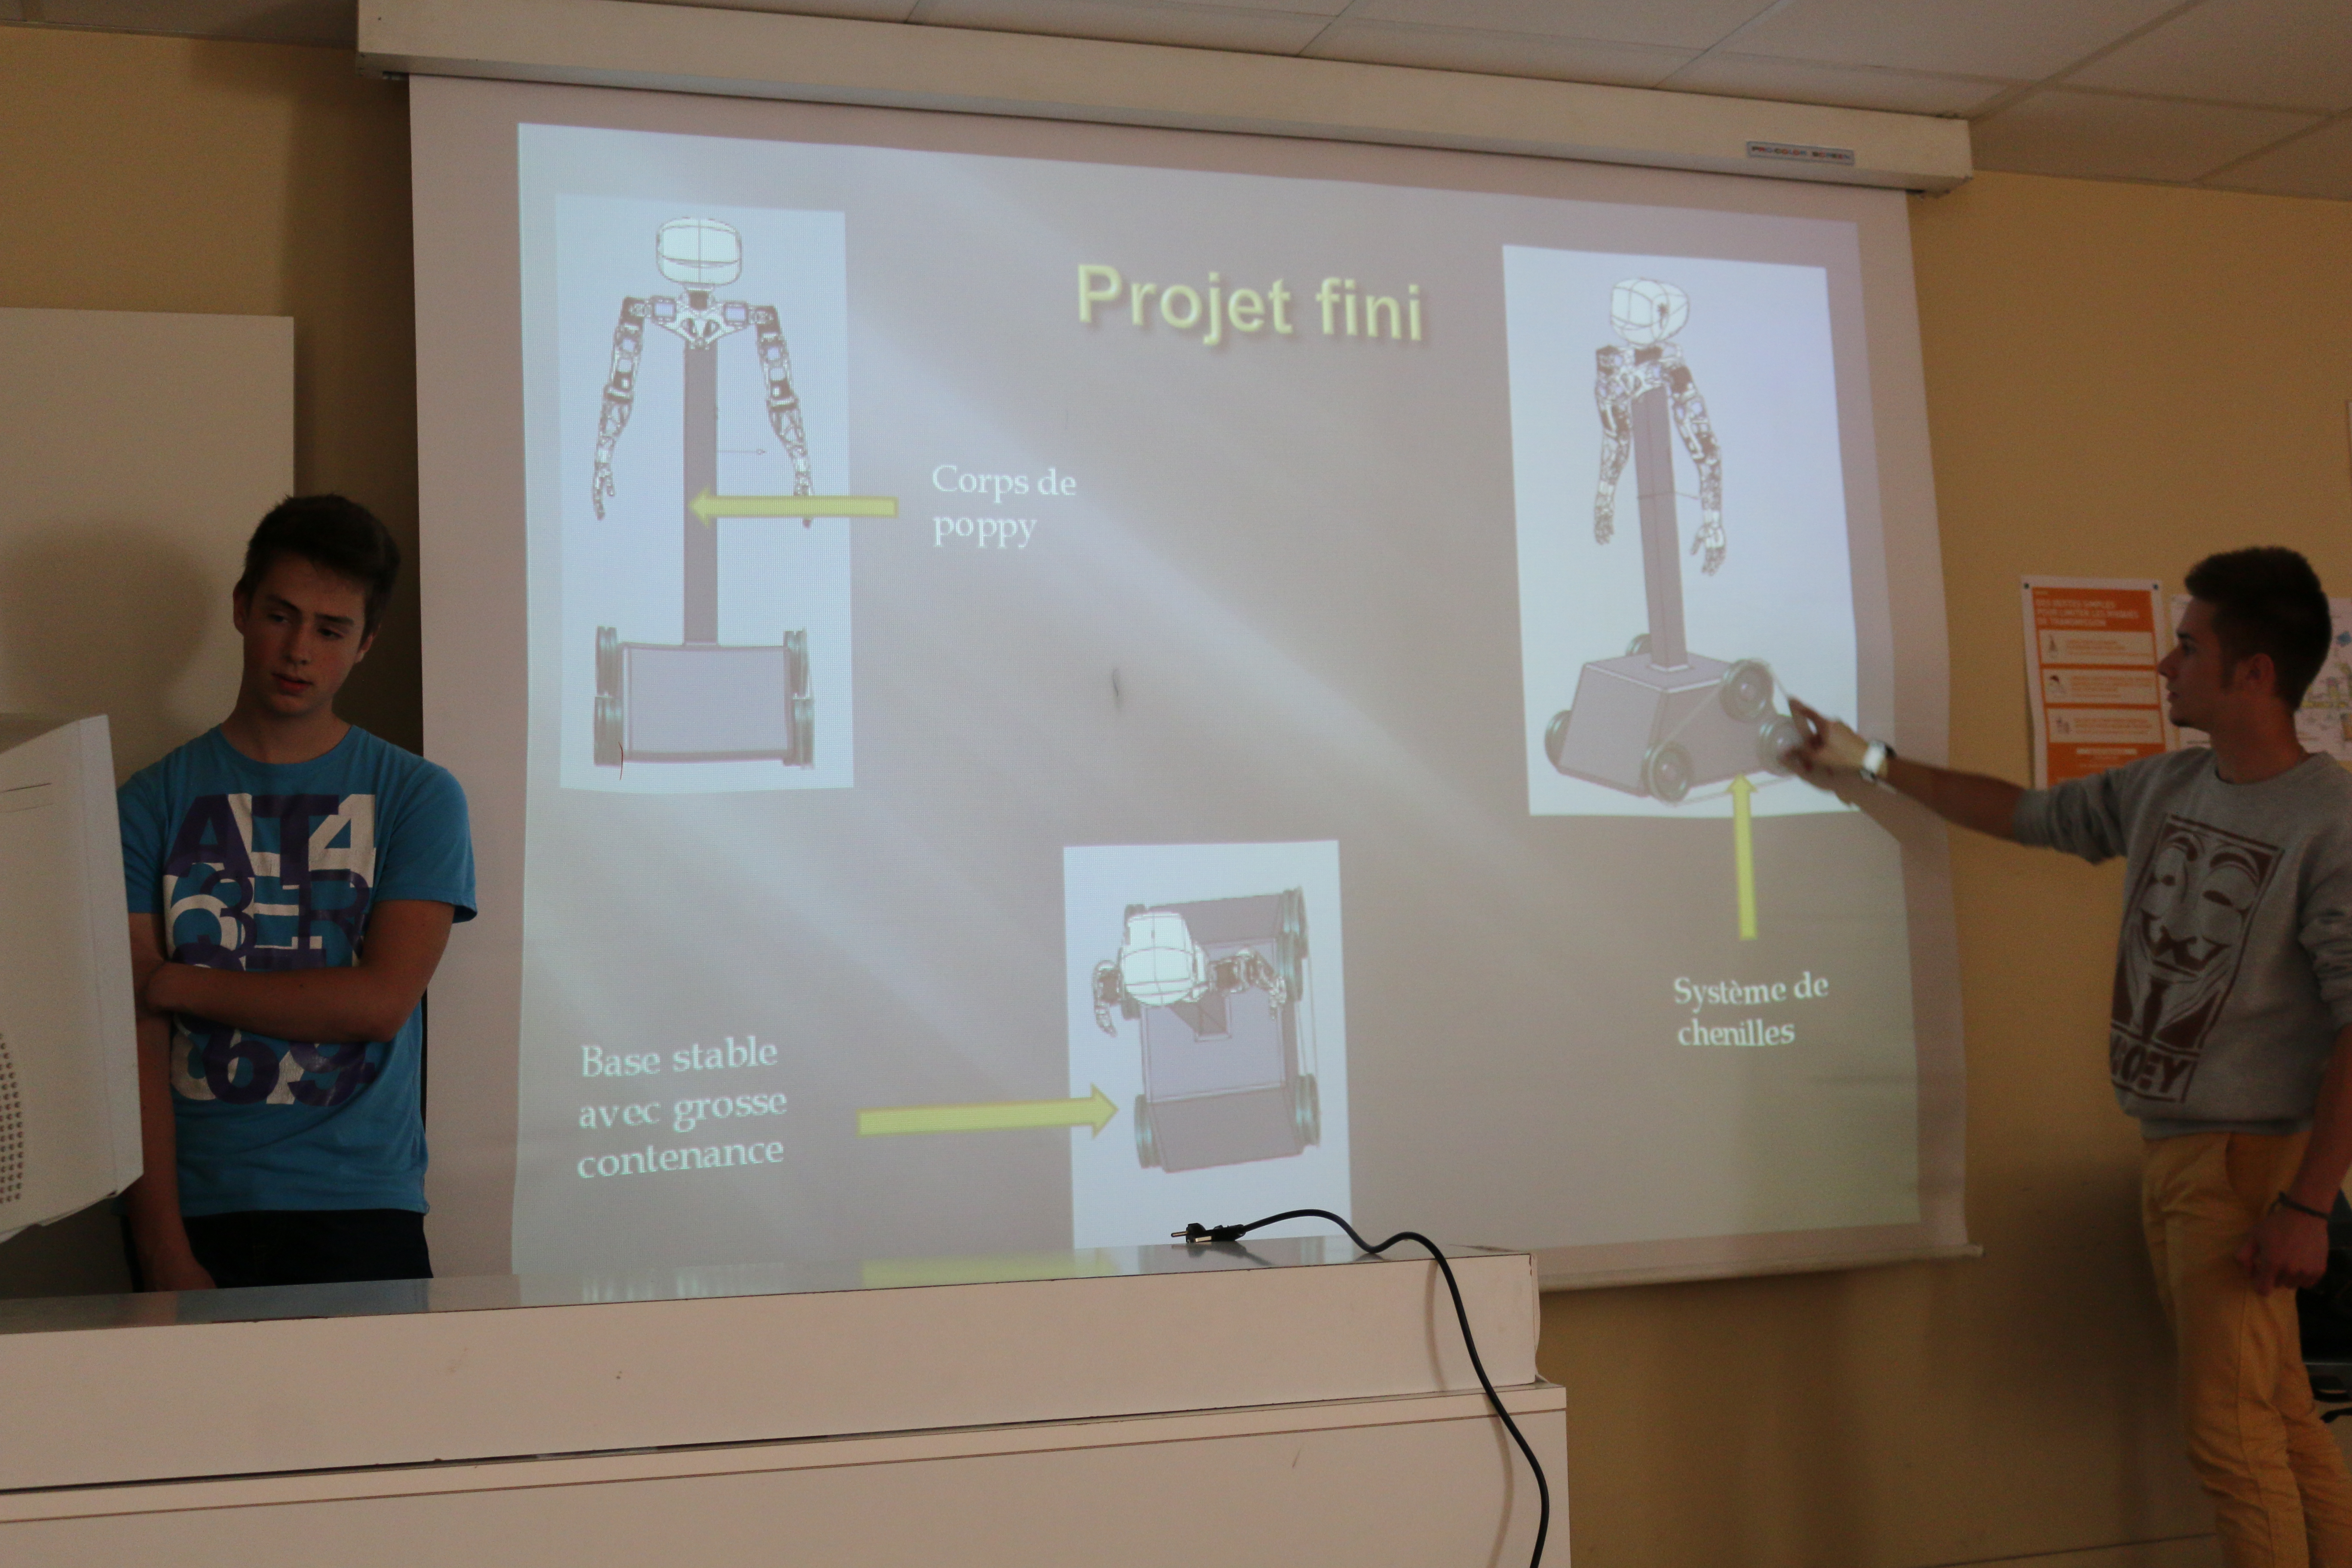
\includegraphics[height=4.5cm]{saintonge_support1.jpg}}
    \hfil
    \subfloat[][Four independant wheel design]{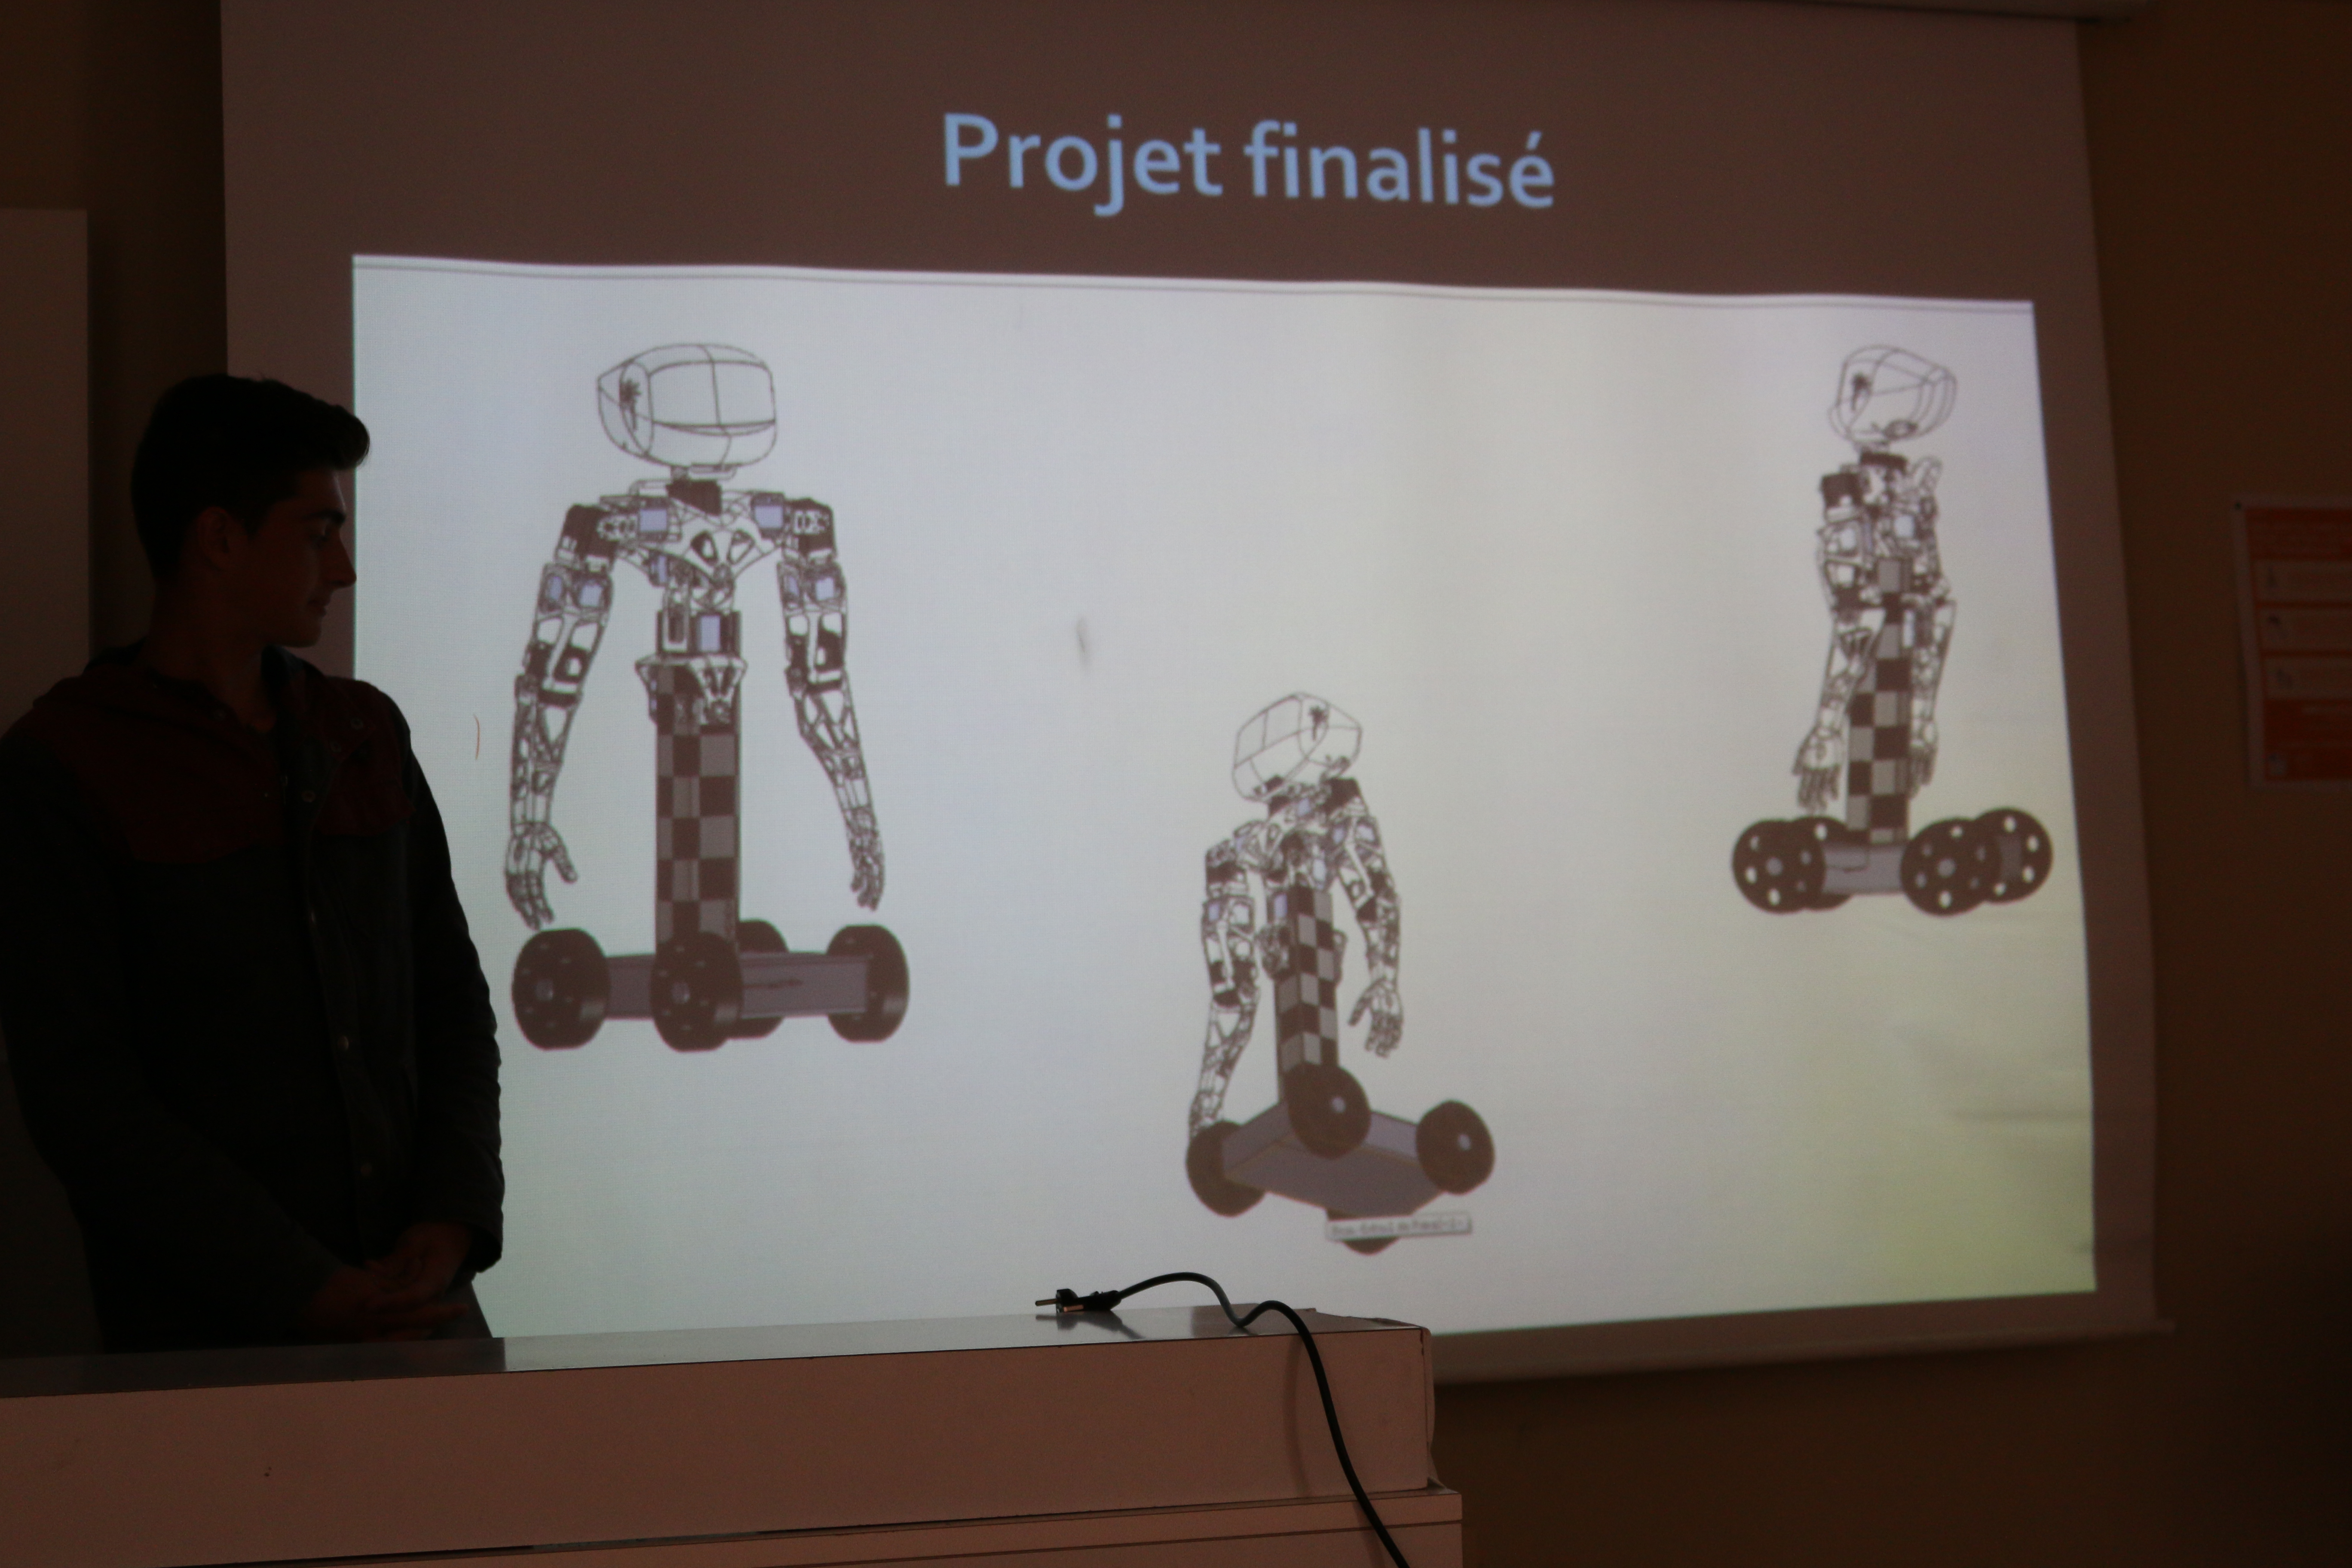
\includegraphics[height=4.5cm]{saintonge_support2.jpg}}
    \hfil
    \subfloat[][Two motorized and a free wheel]{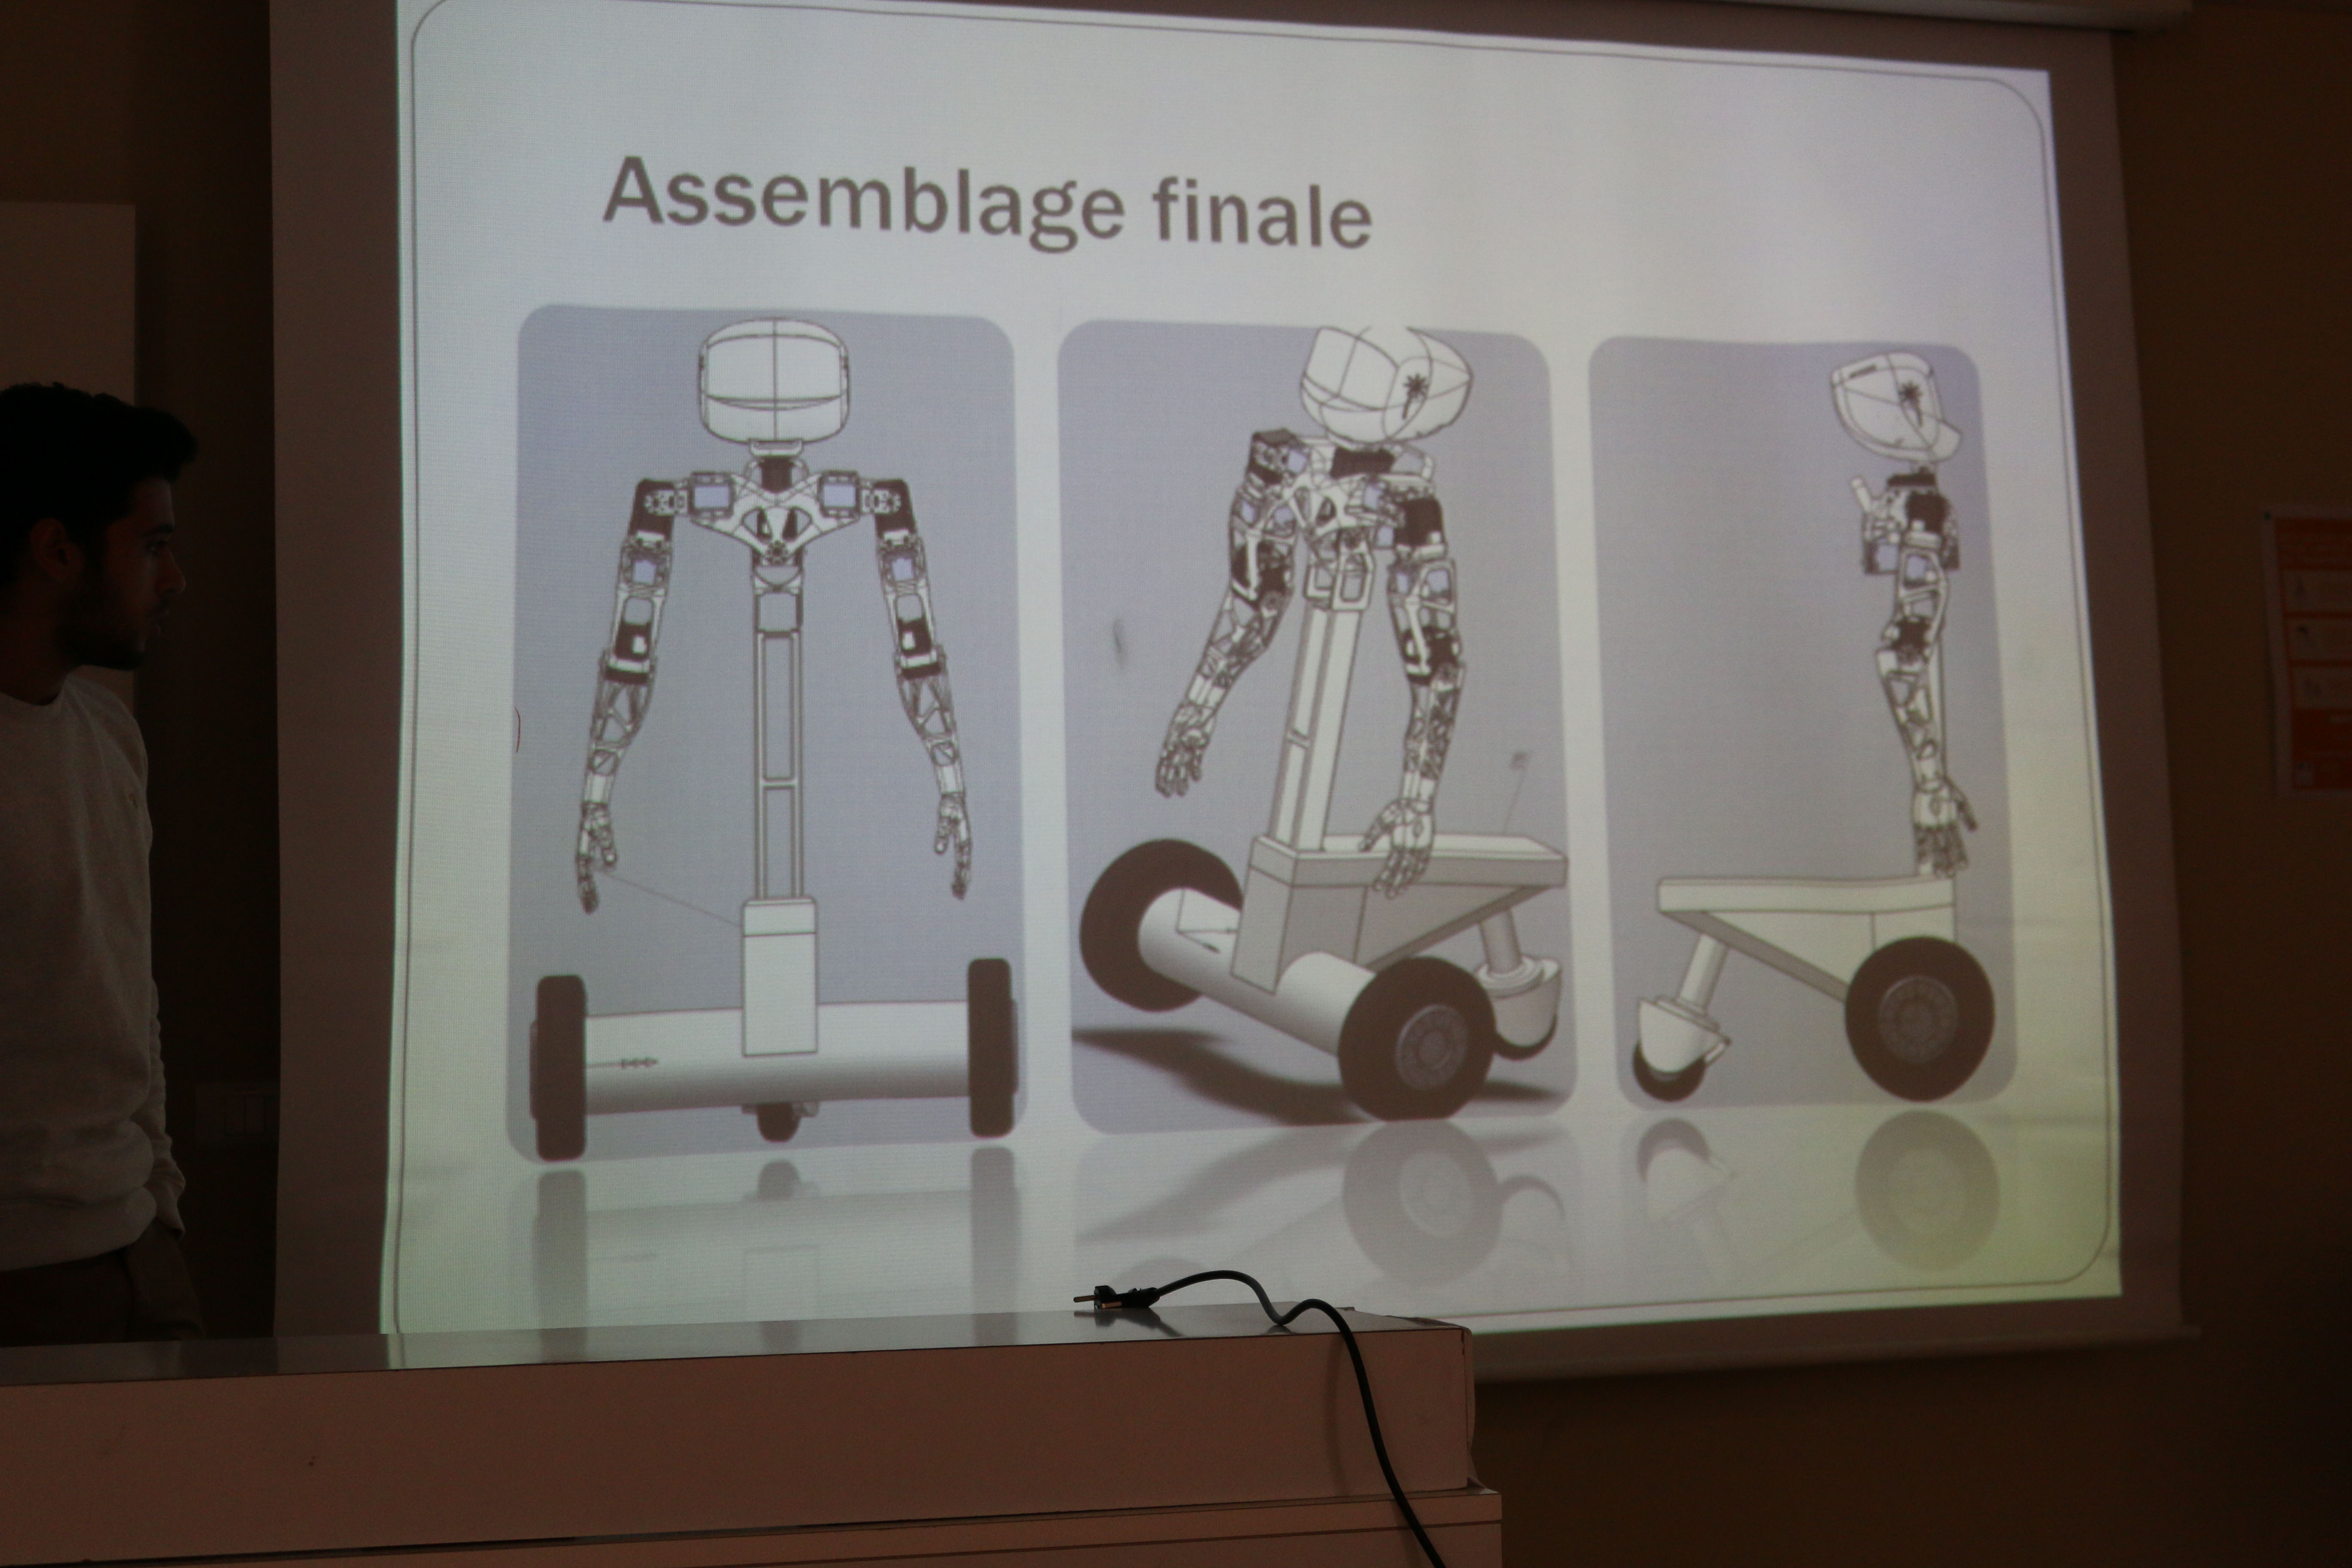
\includegraphics[height=4.5cm]{saintonge_support3.jpg}}
    \caption{Students of the design support work group explain their choices to others.}
    \label{fig:saintonge_support}
\end{figure}


\subsubsection{Documentation and SYSML Diagrams} % (fold)

Finally, the other students were in working groups in charge to report the different workshops. They had to take picture of the robot assembly and get a global view of the project to extract meaningfull information for building SYSML diagrams with MagicDraw.

They had also to train english and report traduction of technical word of the robotic context.


\subsection{Experiment satisfactions} % (fold)

Cette experience avec de jeunes étudiants de parcours professionnel nous a montré que le fait d'avoir un robot "cool" fonctionnel changeait le contexte.

Parler et lire de l'anglais, comprendre des concepts mathematiques, avoir des environnements de dev peu pratique ne les ont pas décourager. D'ailleurs, nous n'avons entendu personne se plaindre des peripéties du projet.

Les moins à l'aise en anglais utilisaient des outils de traductions.




A personnal satisfaction was the fact students worked and learned together, teachning themself.



During this experience, the goal of having a fonctionnal robot was clearly a

Students were never bored to have to go trough classical boring

ça aide a depasser les difficultés techniques. Comprendre le fonctionnement d'un sinus a du sens. On montre que les maths sont utiles.


Plus
\begin{itemize}
    \item Motivation pour depasser les complications d'entrées
    \item une fois l'environnement de travail bien parametré, les gosses arrivent très vite à faire des choses. Pypot est plutôt bien fait pour ça.
    \item POO with object. expliquer les concepts informatiques d'objets avec de vrais objets
    \item On a vu l'interet de prendre des bouts de Poppy.
    \item a la fin je devenais presque inutile, je n'étais là que pour donner un context formel à leur decouverte et aider lors de problème de syntax.
\end{itemize}



\begin{figure}[]
    \begin{center}
        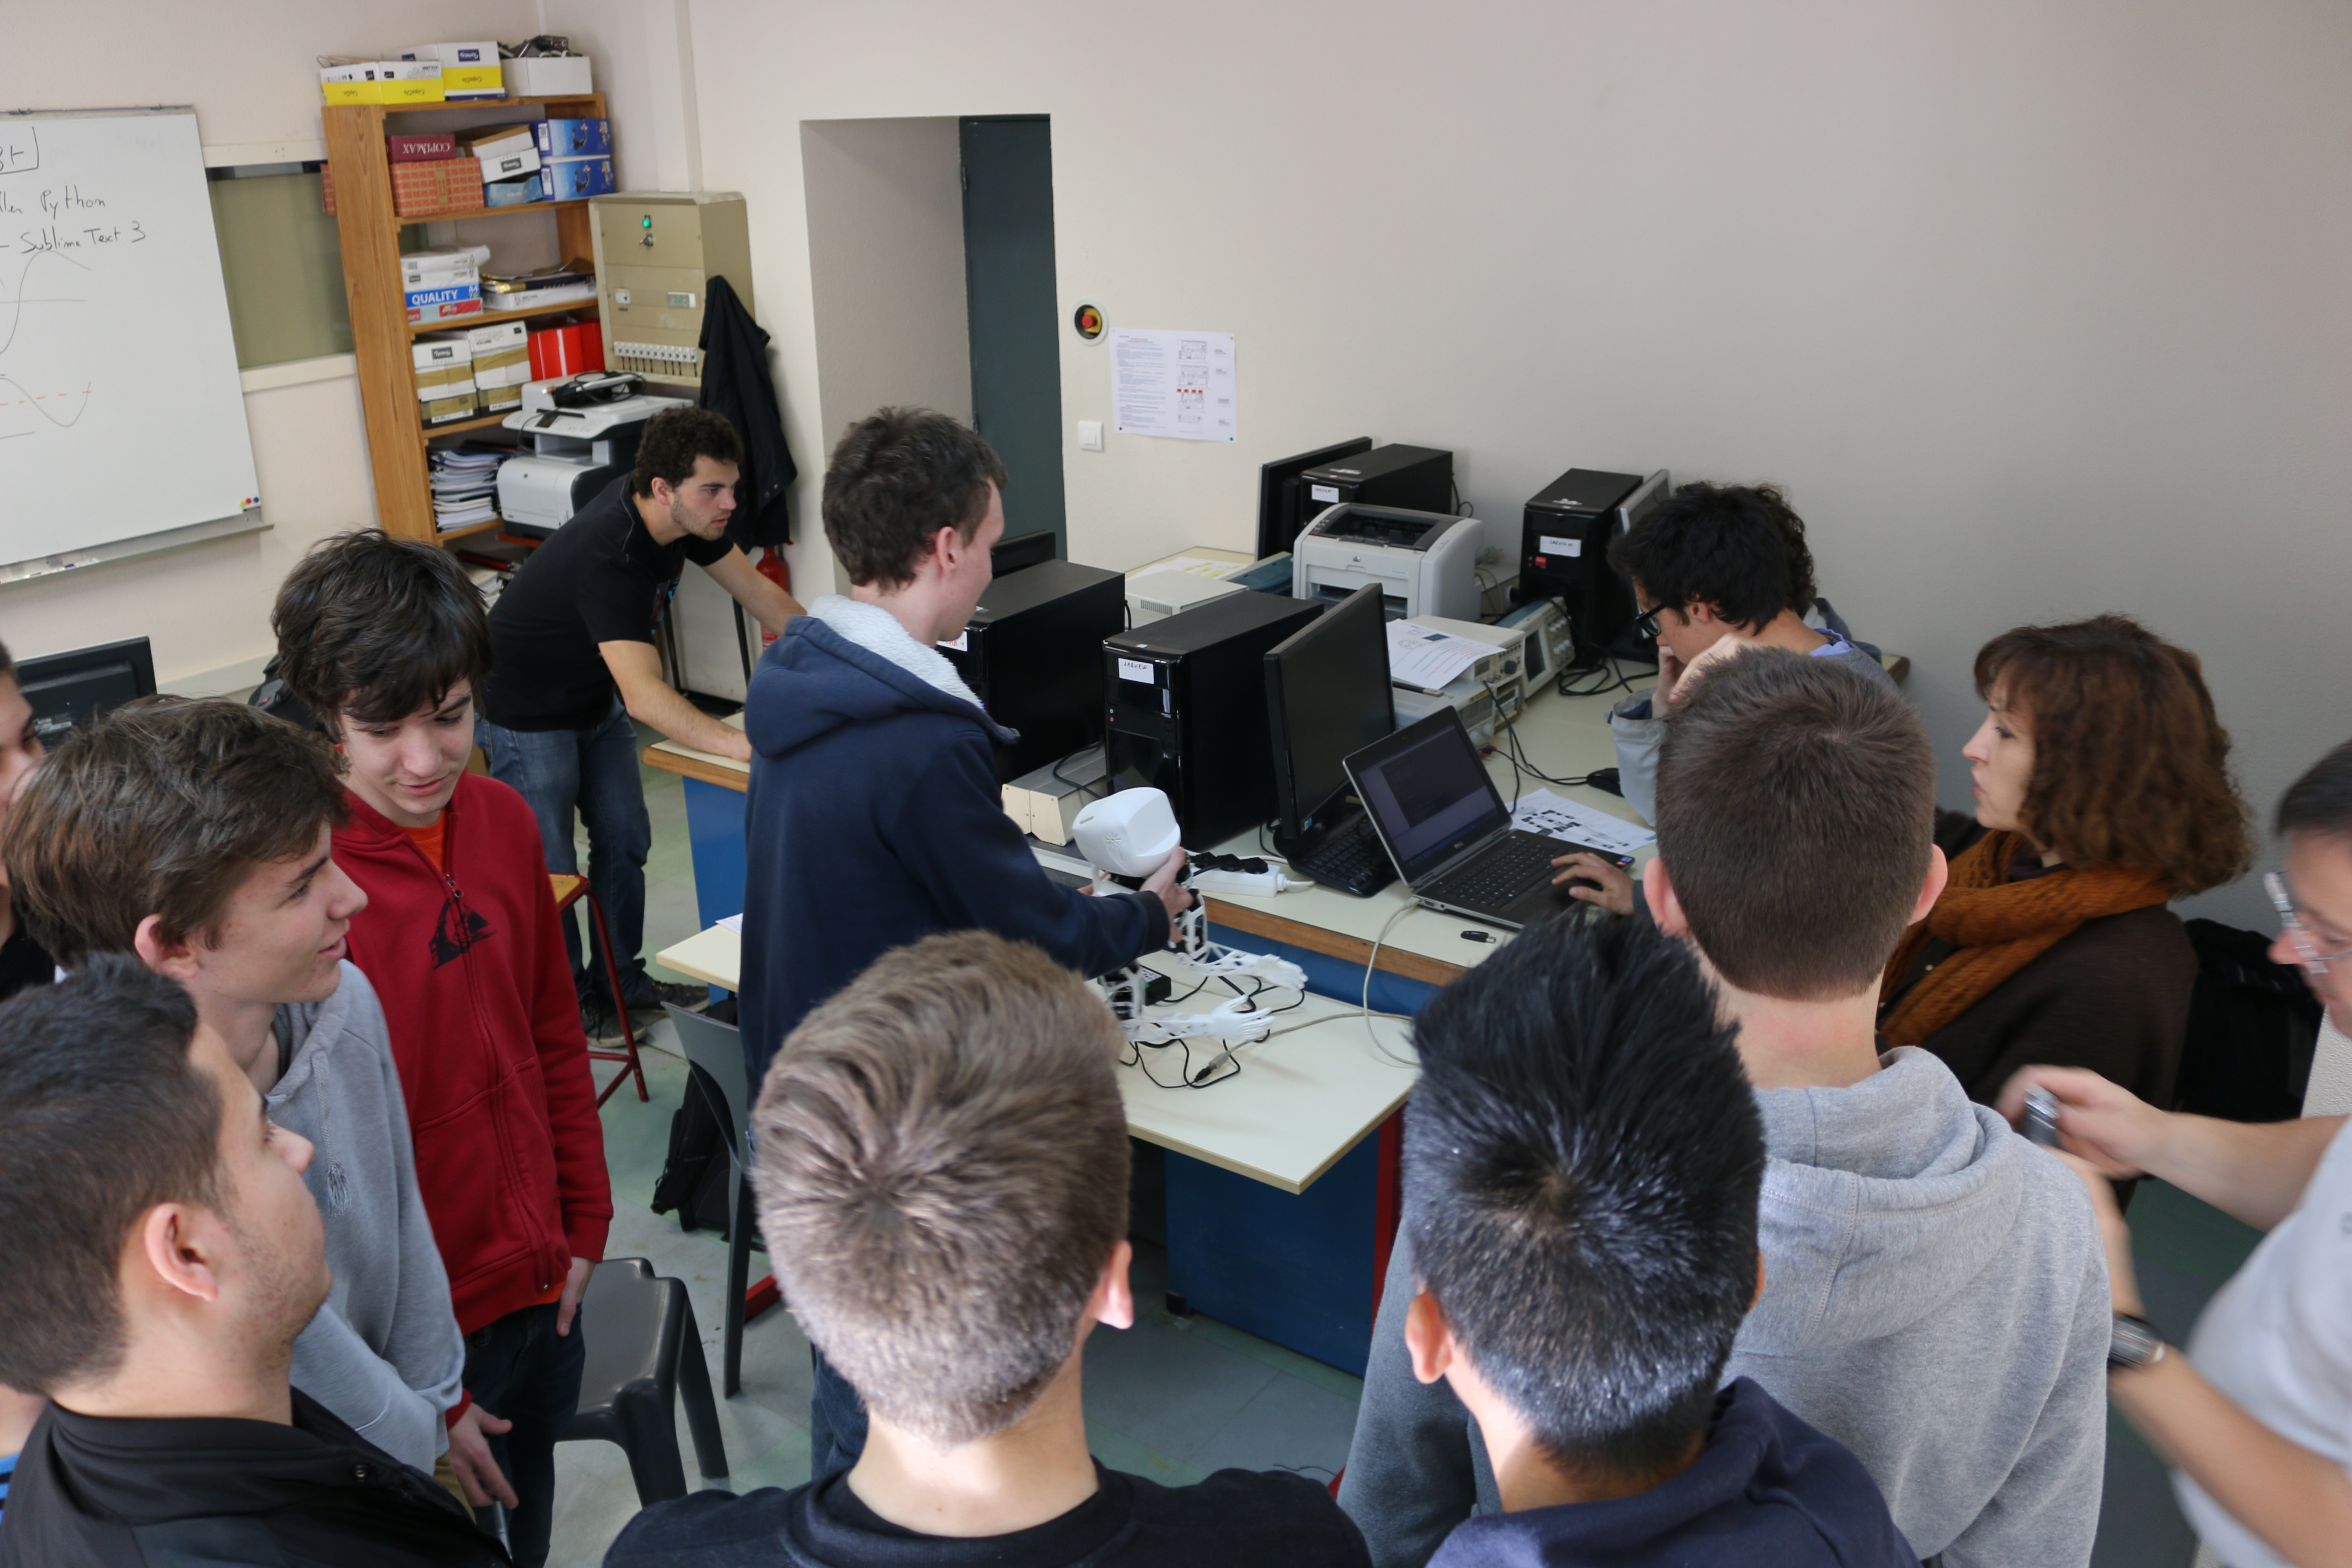
\includegraphics[width=0.8\linewidth]{saintonge_poppy_first_moves.jpg}
    \end{center}
    \caption{Caption here}
    \label{fig:saintonge_result}
\end{figure}

\begin{figure}[]
\centering
    \subfloat[][Constat]{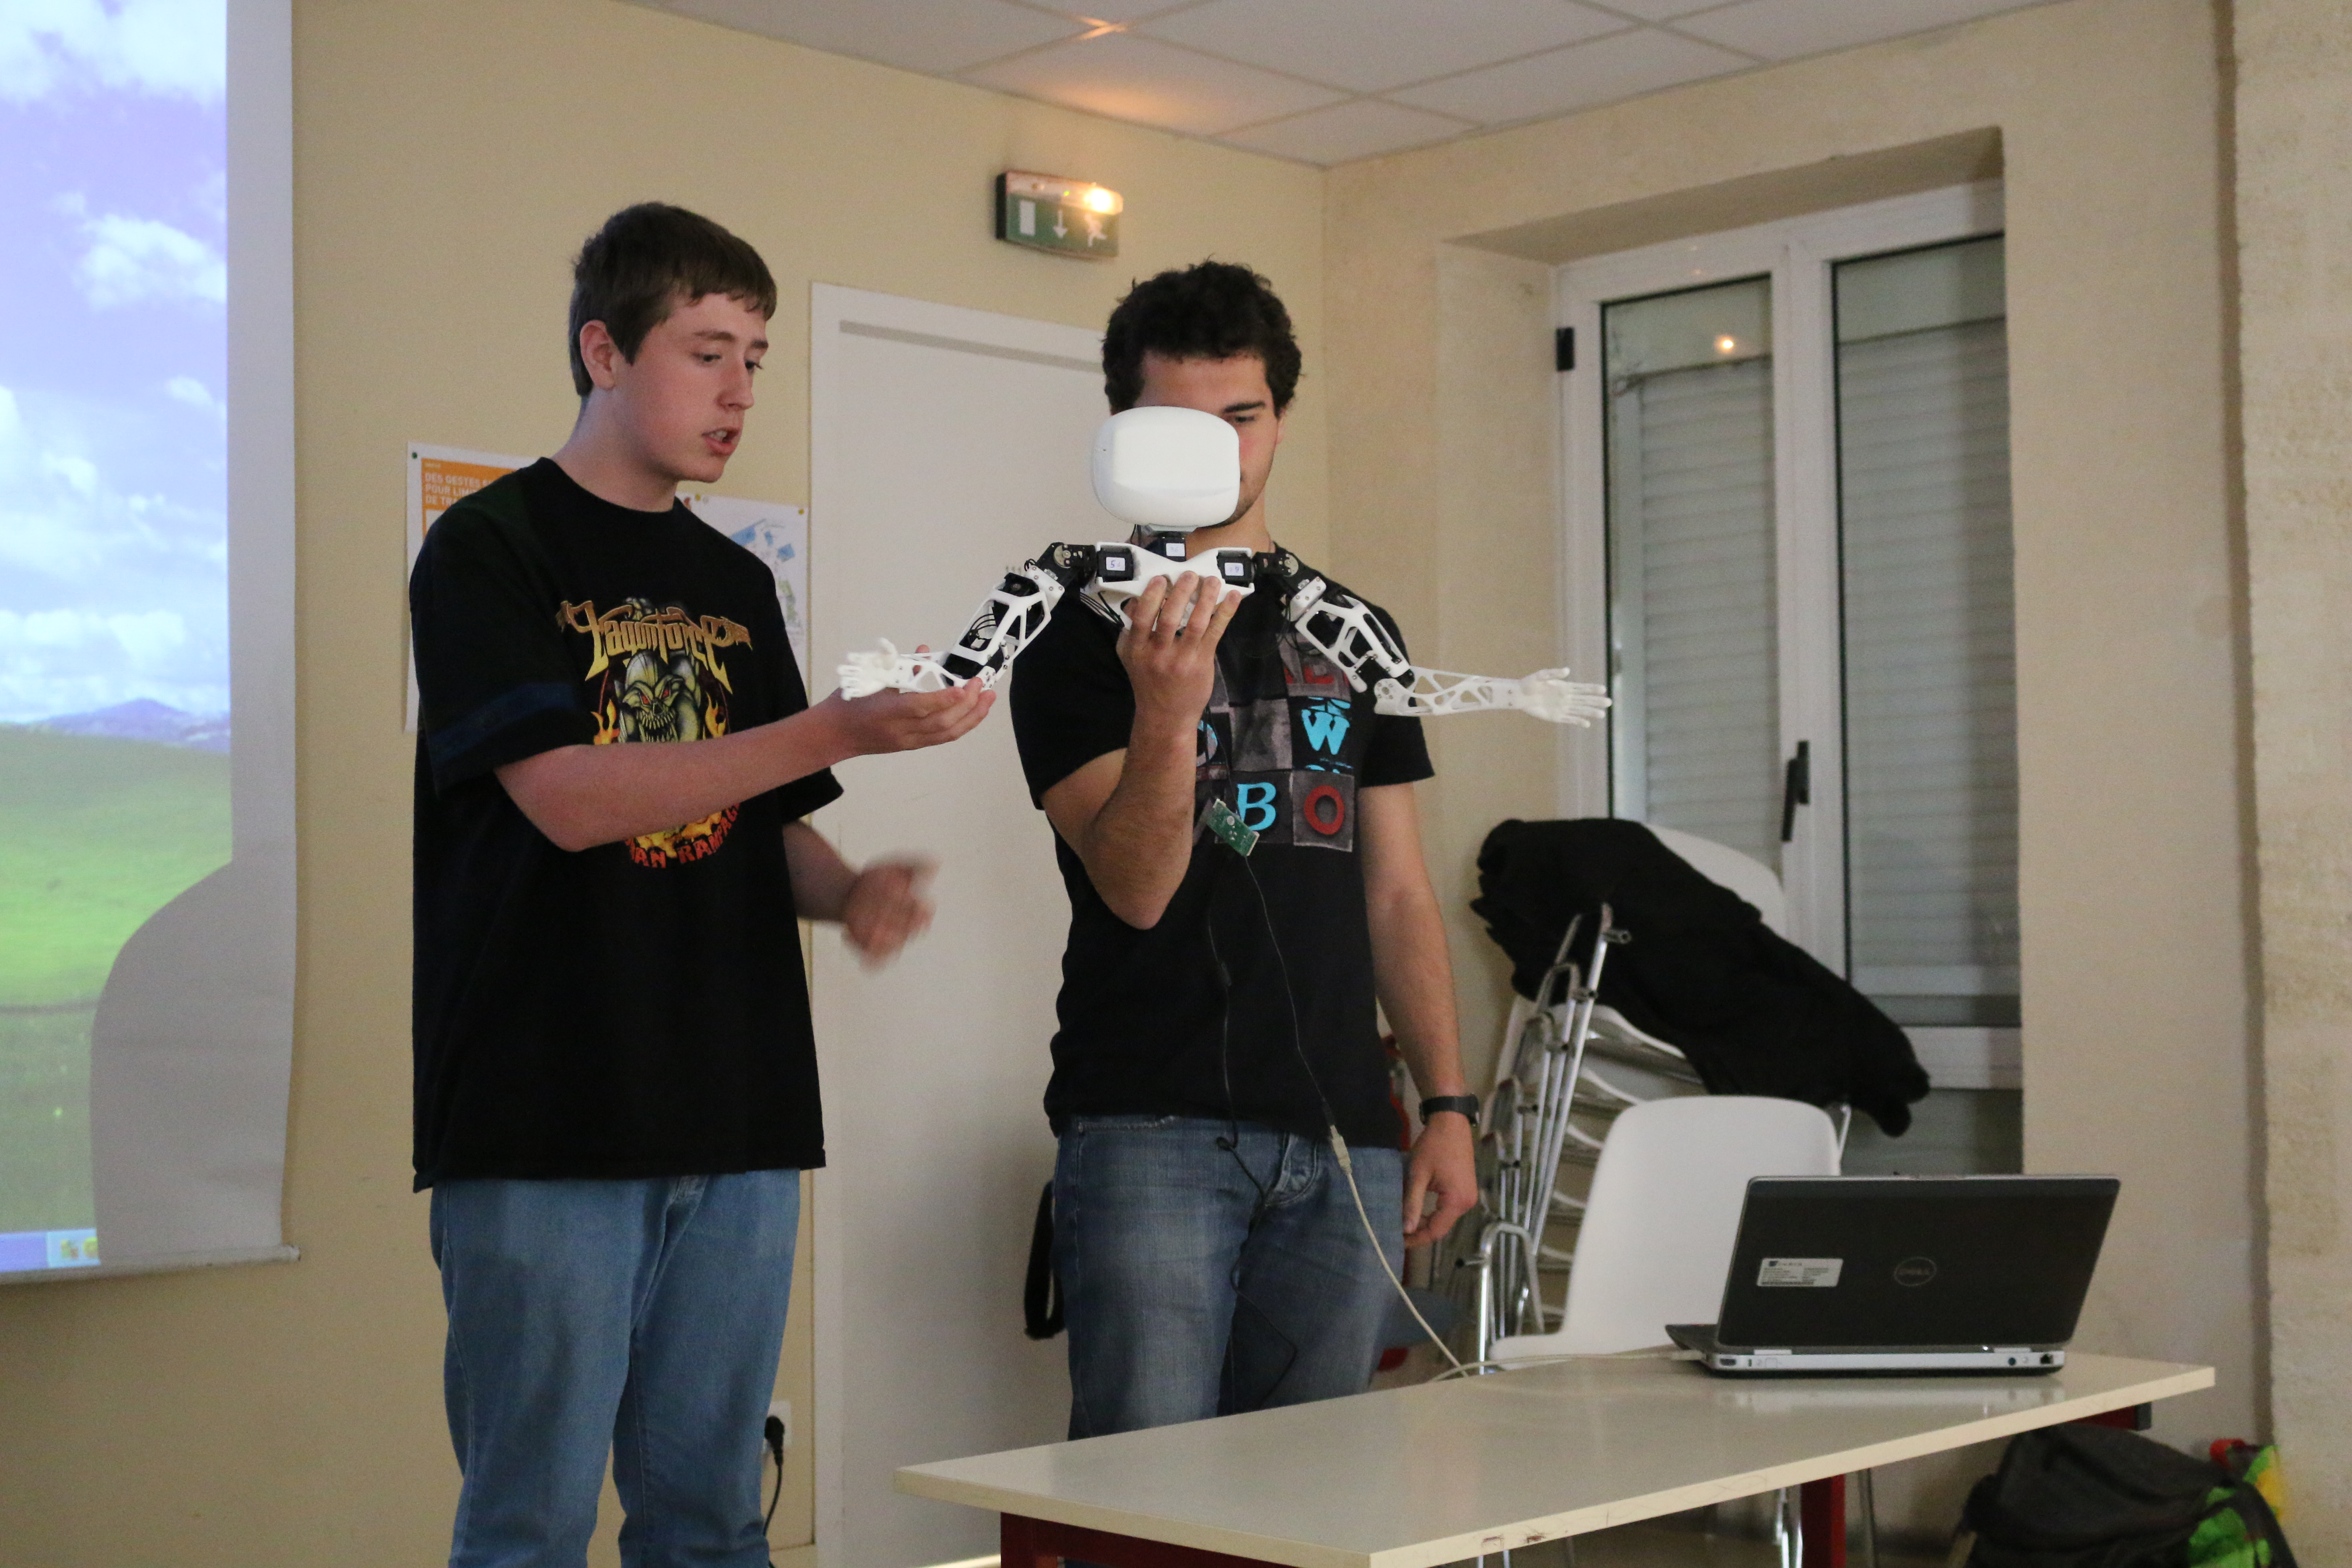
\includegraphics[height=4.3cm]{saintonge_demo1.jpg}}
    \hfil
    \subfloat[][Conception]{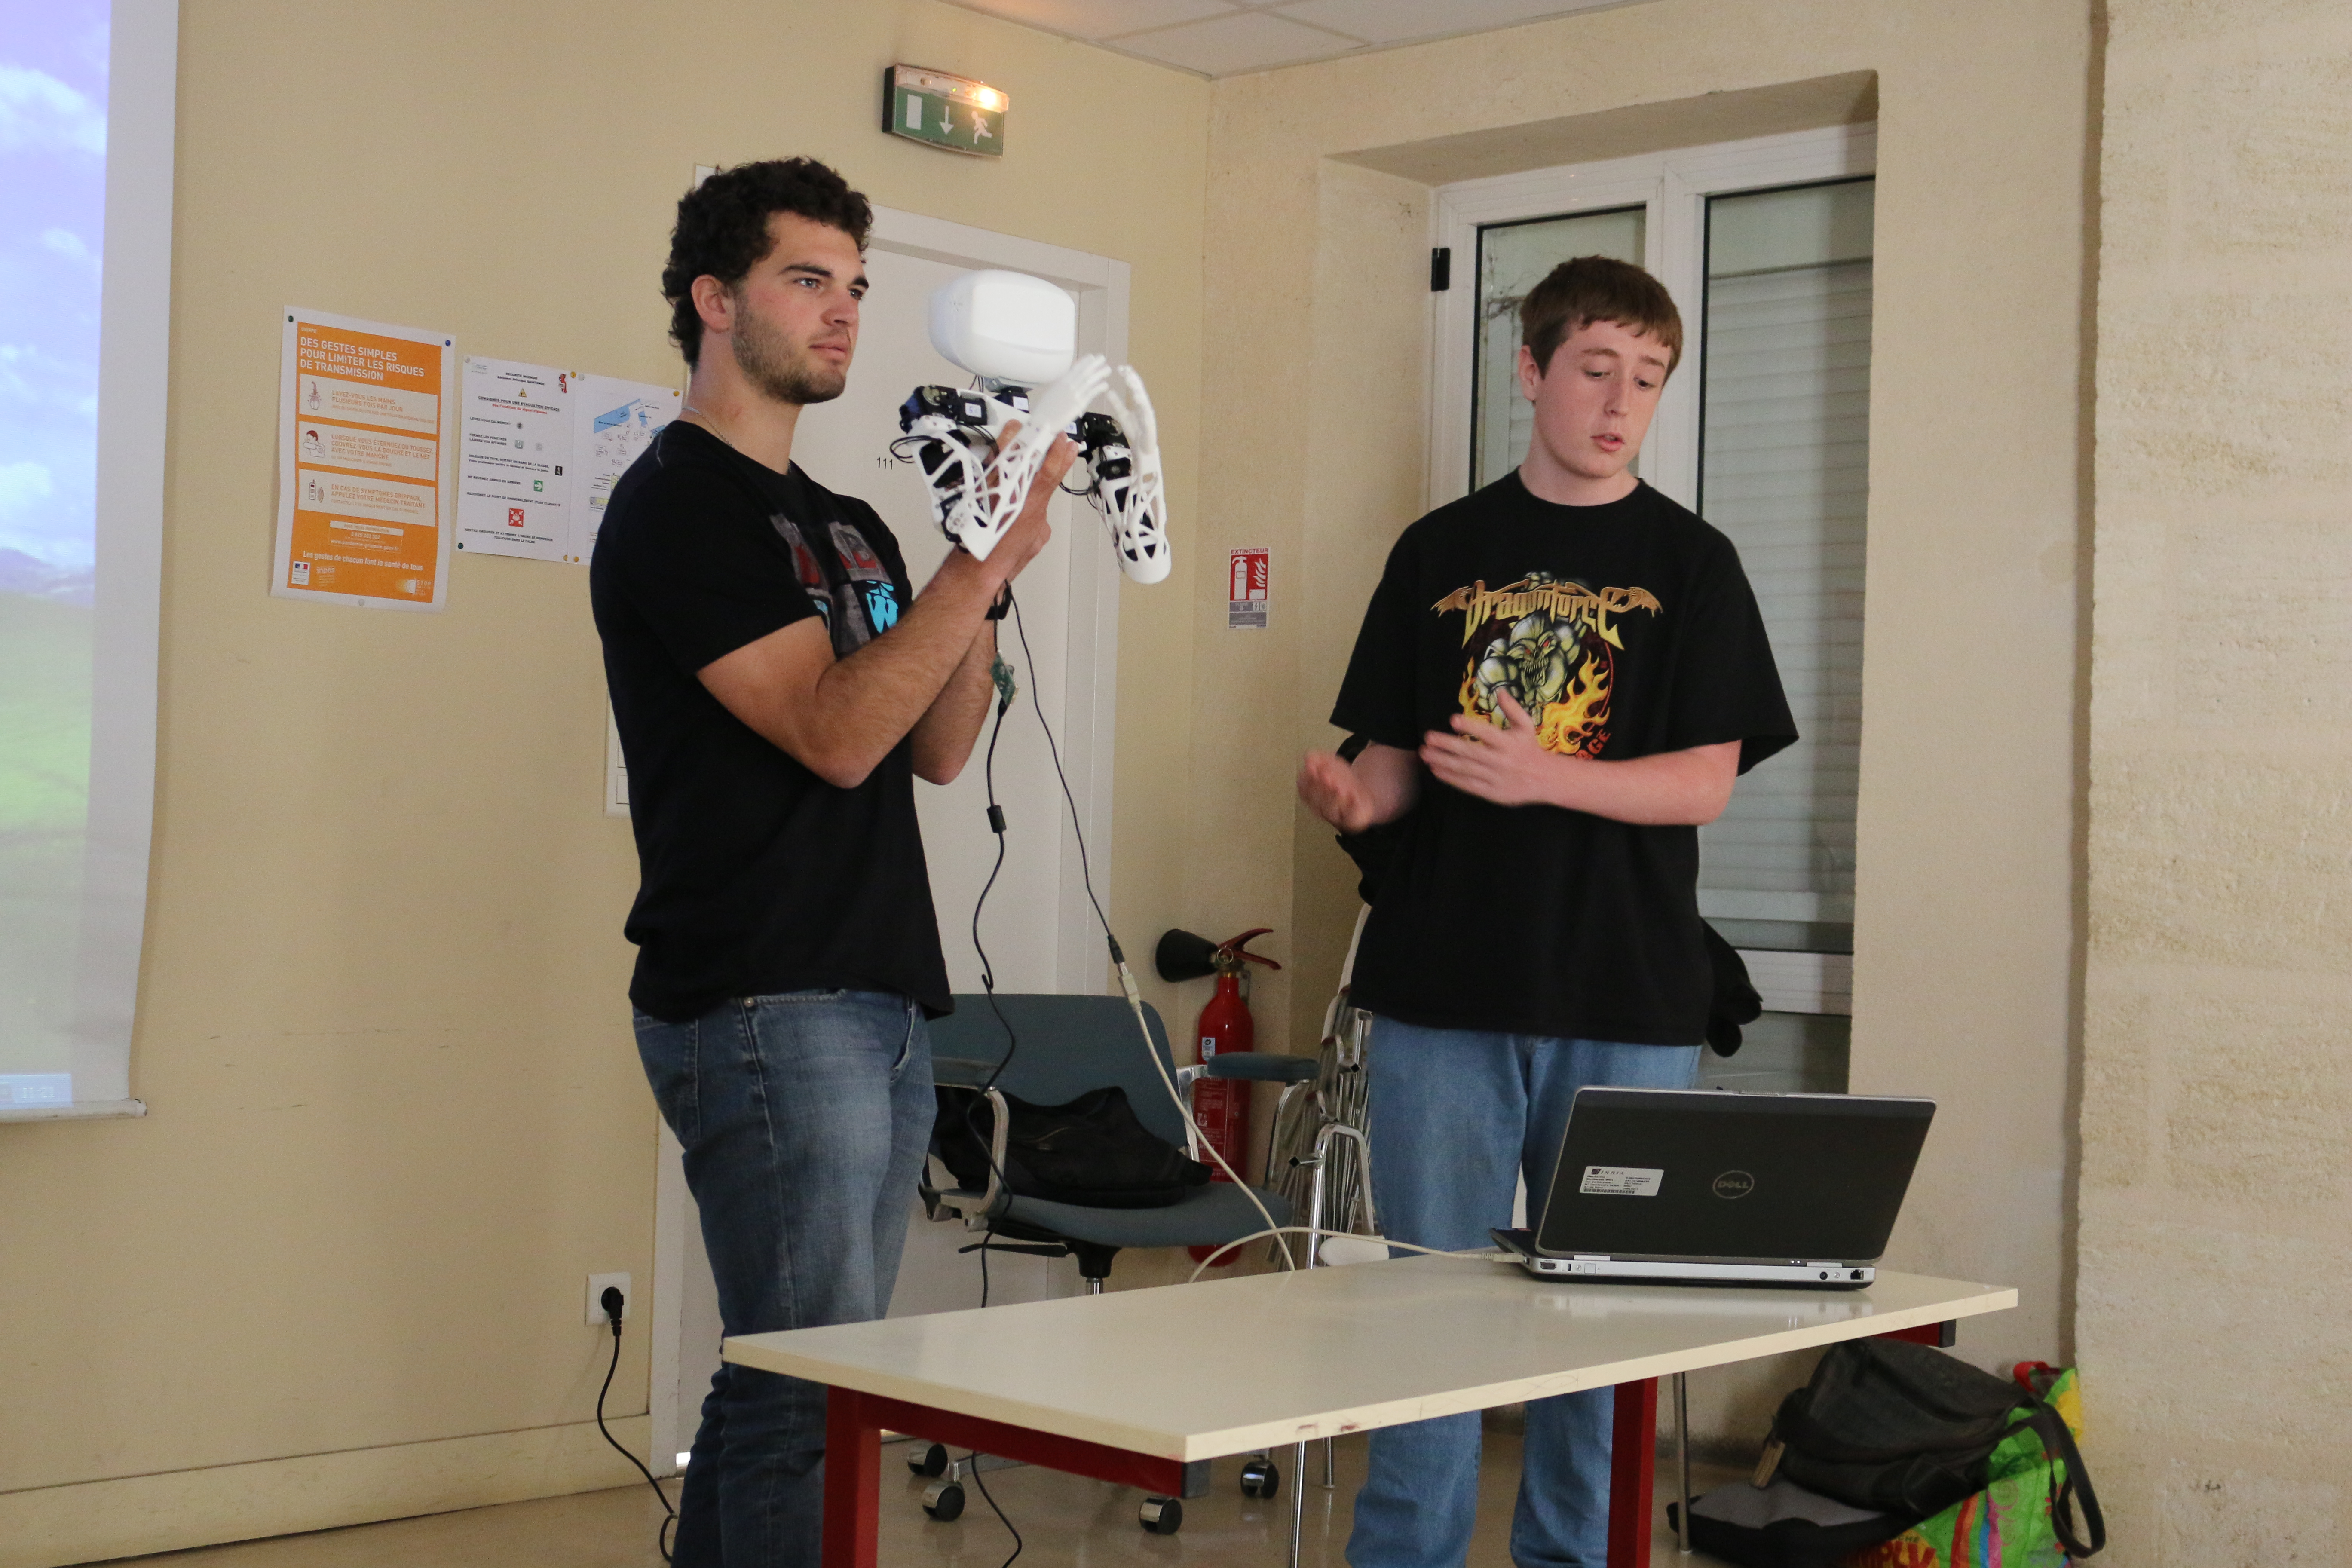
\includegraphics[height=4.3cm]{saintonge_demo2.jpg}}
    \caption{}
    \label{fig:saintonge_demonstration}
\end{figure}




\subsection{Lessons} % (fold)

Internet access was really bad, so slow our forum was not loaded.
We cannot trust school computer. Even if there quite up-to-date, there are used by a lot of users and have potentially incompatibility or weird configuration.


Environnement de developpement seems really important. It is maybe a reason why matlab is more used than python engeering schools.

We should create a stand alone aplication.

Moins

\begin{itemize}
    \item Demande beaucoup d'organisation
    \item certains se retrouvent à ne rien faire
    \item on est à la limite en ce qui concerne le niveau requis. Beaucoup d'inegalité entre les élèves
    \item Problème de PC
    \item il faut trouver un environnement de travail qui ne rend pas plus compliqué le travail des elèves.
\end{itemize}


\section{Conclusion} % (fold)

Il faut faire des fiches d'activités.

Trouver un moyen d'organisation qui permette de repartir la contribution entre les elèves

L'interet d'une platforme aussi compliqué que Poppy est discutable. Il y a peut de chance que des élèves de ce niveau s'interressent à la dynamique passive ou à la compliance

Faire un setup du stand alone.

Peut être faire du Poppy en AX ou un mini Poppy. Dans tout les cas un Poppy tronc serait suffisant.

Flowcode


In ~\cite{resnick2008sowing}, Mitchel Resnick quote the experience a teacher had while using Scratch for a school project.
\begin{quotation}
    There is a buzz in the room when the kids get going on Scratch projects. Students set design goals for their projects and problem-solve to fix program bugs. They collaborate, cooperate, co-teach. They appreciate the power that Scratch gives them to create their own versions of games and animations.

    \signed{Karen Randall, teacher at the Expo Elementary School in~\cite{resnick2008sowing}}
\end{quotation}

This description is actually pretty close from that I experienced with high school students. I was really surprised and pleased how the students were able to go trough a pyramidal way to learn to a flat one or even a bottom-up one.







\section{Conclusion} % (fold)


Open source 3D printed robotic can help creates a meaningful context allowing students to explore several scientific aspect among them, computer science, mechanics and electronics.

We should provide a way to learn where it is

Papert in ~\cite{guzdial2004programming} argued that programming languages should have a low floor (easy to get started with) and a high ceiling (opportunities for increasingly complex projects over time). In addition, we believe that languages need wide walls (supporting many different types of projects, so that people with different interests and learning styles can all become engaged). Satisfying the triplet of low-floor/high-ceiling/wide-walls hasn’t been easy.

Gros challenge autour de l'anglais ...

